% appendixA.tex
% 2010/12/02, v1.20

\chapter{Typesetting appendices}

\section{Single-contributor books}
\subsection{How to typeset one appendix}
If you have just one appendix, say \verb"appendix.tex", you will want to generate a chapter head `Appendix' rather than `Appendix A'. Use \verb"\oneappendix" in the main file, as follows:
\begin{verbatim}
  \oneappendix
  \include{appendix}
\end{verbatim}

\subsection{How to typeset several appendices}
The coding used to generate the appendices in this guide is as follows:
\begin{verbatim}
  \appendix
  % appendixA.tex
% 2010/12/02, v1.20

\chapter{Typesetting appendices}

\section{Single-contributor books}
\subsection{How to typeset one appendix}
If you have just one appendix, say \verb"appendix.tex", you will want to generate a chapter head `Appendix' rather than `Appendix A'. Use \verb"\oneappendix" in the main file, as follows:
\begin{verbatim}
  \oneappendix
  \include{appendix}
\end{verbatim}

\subsection{How to typeset several appendices}
The coding used to generate the appendices in this guide is as follows:
\begin{verbatim}
  \appendix
  % appendixA.tex
% 2010/12/02, v1.20

\chapter{Typesetting appendices}

\section{Single-contributor books}
\subsection{How to typeset one appendix}
If you have just one appendix, say \verb"appendix.tex", you will want to generate a chapter head `Appendix' rather than `Appendix A'. Use \verb"\oneappendix" in the main file, as follows:
\begin{verbatim}
  \oneappendix
  \include{appendix}
\end{verbatim}

\subsection{How to typeset several appendices}
The coding used to generate the appendices in this guide is as follows:
\begin{verbatim}
  \appendix
  % appendixA.tex
% 2010/12/02, v1.20

\chapter{Typesetting appendices}

\section{Single-contributor books}
\subsection{How to typeset one appendix}
If you have just one appendix, say \verb"appendix.tex", you will want to generate a chapter head `Appendix' rather than `Appendix A'. Use \verb"\oneappendix" in the main file, as follows:
\begin{verbatim}
  \oneappendix
  \include{appendix}
\end{verbatim}

\subsection{How to typeset several appendices}
The coding used to generate the appendices in this guide is as follows:
\begin{verbatim}
  \appendix
  \include{appendixA}
  \include{appendixB}
  \include{appendixC}
\end{verbatim}

\section{Multi-contributor books}

\subsection{How to typeset one appendix}
If you have just one appendix, it will be the next section head and you should include the following code at the end of your chapter:
\begin{verbatim}
  \oneappendix
  \section{Appendix heading}
  \subsection{Subheading}
  \endappendix
\end{verbatim}
You will need to add \verb"\endappendix" if you have further section heads in this chapter.


\subsection{How to typeset several appendices}
The following code will genenerate Appendix~A and Appendix~B at the end of your chapter:
\begin{verbatim}
  \appendix
  \section{Appendix heading}
  \subsection{Subheading}
    :
  \section{Next appendix heading}
  \subsection{Next subheading}
  \endappendix
\end{verbatim}
Again, you will need to add \verb"\endappendix" if you have further section heads in this chapter.

\section{Numbering systems}

Equations in appendices will be numbered as follows:
\begin{equation}
  E=mc^2,
\end{equation}
and figure captions as follows:
\begin{figure}[h]
\caption{Similarity solutions}
\end{figure}

\endinput
  % appendixB.tex
% 2010/12/02, v1.20

\chapter{amsthm commands}
\label{amsthmcommands}

The following code may be cut and pasted into your root file. Assuming you have included \verb"amsthm.sty", it will number your theorems, definitions, etc. in the same numbering sequence and by chapter, e.g.~Definition~4.1, Lemma~4.2, Lemma~4.3, Proposition~4.4, Corollary~4.5.

If you prefer to have the elements numbered by section, e.g.~Definition~4.1.1, Lemma~4.1.2, Lemma~4.1.3, Proposition~4.1.4, Corollary~4.1.5, replace \verb"[chapter]" on line 2 with \verb"[section]".

\begin{smallverbatim}

  \theoremstyle{plain}% default
  \newtheorem{theorem}{Theorem}[chapter]
  \newtheorem{lemma}[theorem]{Lemma}
  \newtheorem{corollary}[theorem]{Corollary}
  \newtheorem{proposition}[theorem]{Proposition}
  \newtheorem{conjecture}[theorem]{Conjecture}
  \newtheorem{criterion}[theorem]{Criterion}
  \newtheorem{algorithm}[theorem]{Algorithm}

  \theoremstyle{definition}
  \newtheorem{definition}[theorem]{Definition}
  \newtheorem{condition}[theorem]{Condition}

  \theoremstyle{remark}
  \newtheorem{remark}[theorem]{Remark}
  \newtheorem{note}[theorem]{Note}
  \newtheorem{notation}[theorem]{Notation}
  \newtheorem{claim}[theorem]{Claim}
  \newtheorem{summary}[theorem]{Summary}
  \newtheorem{acknowledgement}[theorem]{Acknowledgement}
  \newtheorem{case}[theorem]{Case}
  \newtheorem{conclusion}[theorem]{Conclusion}
\end{smallverbatim}

\endinput
  % appendixC.tex
% 2010/12/02, v1.20

\chapter{The root file for this~guide}
\label{rootfile}

\vfill
\begin{smallverbatim}
% PT1guide.tex
% for the suite of standard Cambridge designs
% 2010/12/02, v1.20

  \NeedsTeXFormat{LaTeX2e}[1996/06/01]

% \documentclass[multi]{PT1}  % multi-contributor option
% \documentclass[prodtf]{PT1} % production option (used to produce PT1guide.pdf);
                              % can only be used if you have the Adobe Myriad Pro
                              % condensed font
  \documentclass{PT1}
  \usepackage{natbib}
  \usepackage[figuresright]{rotating}
  \usepackage{floatpag}
    \rotfloatpagestyle{empty}

% \usepackage{amsmath}        % if you are using this package,
                              % it must be loaded before amsthm.sty
  \usepackage{amsthm}

% \usepackage{txfonts}        % times font (used to produce PT1guide.pdf)

% indexes
% uncomment the relevant set of commands

% for a single index
% \usepackage{makeidx}
% \makeindex

% for multiple indexes using multind.sty
  \usepackage{multind}\ProvidesPackage{multind}
  \makeindex{authors}
  \makeindex{subject}

% for multiple indexes using index.sty
% \usepackage{index}
% \newindex{aut}{adx}{and}{Author index}
% \makeindex

  \newcommand\cambridge{PT1}

% see chapter 3 for details
  \theoremstyle{plain}% default
  \newtheorem{theorem}{Theorem}[chapter]
  \newtheorem{lemma}[theorem]{Lemma}
  \newtheorem*{corollary}{Corollary}

  \theoremstyle{definition}
  \newtheorem{definition}[theorem]{Definition}
  \newtheorem{condition}[theorem]{Condition}
  \newtheorem{example-norules}[theorem]{Example}%

  \theoremstyle{remark}
  \newtheorem*{remark}{Remark}
  \newtheorem*{case}{Case}

  \hyphenation{line-break line-breaks docu-ment triangle cambridge
    amsthdoc cambridgemods baseline-skip author authors
    cambridgestyle en-vir-on-ment polar astron-omers solu-tion}

  \setcounter{tocdepth}{2}    % the toc normally lists sections; for the purposes of
                              % this document, this has been extended to subsections

%%%%%%%%%%%%%%%%%%%%%%%%%%%%%%%%%%%%%

% \includeonly{chap2}

%%%%%%%%%%%%%%%%%%%%%%%%%%%%%%%%%%%%%

  \begin{document}

  \title[Subtitle, If You Have One]
    {\LaTeXeintitle\ Guide for Authors using~the~\cambridge~Design}

  \author{Ali Woollatt}

  \details{This guide was compiled using \cambridge.cls \version\\[\baselineskip]
    The latest version can be downloaded from:
    https://authornet.cambridge.org/information/productionguide/
      LaTeX\_files/\cambridge.zip}

  \frontmatter
  \maketitle
  \tableofcontents
  \listoffigures
  \listoftables
  \listoffloatingboxes
  \listofcontributors

  \mainmatter
  \partquote{I have called this principle, by which each slight variation,
    if useful, is preserved, by the term of Natural Selection.}{Charles Darwin}
    \label{partquote}
  \part{Getting started}
  \include{chap1}% introduction
  \include{chap2}% features of the \cambridge\ class file
  \include{chap3}% mathematical solutions

  \addtocontents{toc}{\protect\pagebreak}
  \part{Closing features}
  \include{chap4}% references and bibliographies
  \include{chap5}% single and multiple indexes

  \backmatter
% if you only have one appendix, use \oneappendix instead of \appendix

  \appendix
  \include{appendixA}
  \include{appendixB}
  \include{appendixC}
  \endappendix

% insert a blank line to the toc list
  \addtocontents{toc}{\vspace{\baselineskip}}
  \theendnotes

% \renewcommand{\refname}{Bibliography}% if you prefer this heading
  \bibliography{percolation}\label{refs}
  \bibliographystyle{cambridgeauthordate}

  \cleardoublepage

% indexes

% for a single index
% \printindex

% for multiple indexes using multind.sty
  \printindex{authors}{Author index}
  \printindex{subject}{Subject index}

% for multiple indexes using index.sty
% \printindex[aut]
% \printindex

\end{document}
\end{smallverbatim}
\endinput
\end{verbatim}

\section{Multi-contributor books}

\subsection{How to typeset one appendix}
If you have just one appendix, it will be the next section head and you should include the following code at the end of your chapter:
\begin{verbatim}
  \oneappendix
  \section{Appendix heading}
  \subsection{Subheading}
  \endappendix
\end{verbatim}
You will need to add \verb"\endappendix" if you have further section heads in this chapter.


\subsection{How to typeset several appendices}
The following code will genenerate Appendix~A and Appendix~B at the end of your chapter:
\begin{verbatim}
  \appendix
  \section{Appendix heading}
  \subsection{Subheading}
    :
  \section{Next appendix heading}
  \subsection{Next subheading}
  \endappendix
\end{verbatim}
Again, you will need to add \verb"\endappendix" if you have further section heads in this chapter.

\section{Numbering systems}

Equations in appendices will be numbered as follows:
\begin{equation}
  E=mc^2,
\end{equation}
and figure captions as follows:
\begin{figure}[h]
\caption{Similarity solutions}
\end{figure}

\endinput
  % appendixB.tex
% 2010/12/02, v1.20

\chapter{amsthm commands}
\label{amsthmcommands}

The following code may be cut and pasted into your root file. Assuming you have included \verb"amsthm.sty", it will number your theorems, definitions, etc. in the same numbering sequence and by chapter, e.g.~Definition~4.1, Lemma~4.2, Lemma~4.3, Proposition~4.4, Corollary~4.5.

If you prefer to have the elements numbered by section, e.g.~Definition~4.1.1, Lemma~4.1.2, Lemma~4.1.3, Proposition~4.1.4, Corollary~4.1.5, replace \verb"[chapter]" on line 2 with \verb"[section]".

\begin{smallverbatim}

  \theoremstyle{plain}% default
  \newtheorem{theorem}{Theorem}[chapter]
  \newtheorem{lemma}[theorem]{Lemma}
  \newtheorem{corollary}[theorem]{Corollary}
  \newtheorem{proposition}[theorem]{Proposition}
  \newtheorem{conjecture}[theorem]{Conjecture}
  \newtheorem{criterion}[theorem]{Criterion}
  \newtheorem{algorithm}[theorem]{Algorithm}

  \theoremstyle{definition}
  \newtheorem{definition}[theorem]{Definition}
  \newtheorem{condition}[theorem]{Condition}

  \theoremstyle{remark}
  \newtheorem{remark}[theorem]{Remark}
  \newtheorem{note}[theorem]{Note}
  \newtheorem{notation}[theorem]{Notation}
  \newtheorem{claim}[theorem]{Claim}
  \newtheorem{summary}[theorem]{Summary}
  \newtheorem{acknowledgement}[theorem]{Acknowledgement}
  \newtheorem{case}[theorem]{Case}
  \newtheorem{conclusion}[theorem]{Conclusion}
\end{smallverbatim}

\endinput
  % appendixC.tex
% 2010/12/02, v1.20

\chapter{The root file for this~guide}
\label{rootfile}

\vfill
\begin{smallverbatim}
% PT1guide.tex
% for the suite of standard Cambridge designs
% 2010/12/02, v1.20

  \NeedsTeXFormat{LaTeX2e}[1996/06/01]

% \documentclass[multi]{PT1}  % multi-contributor option
% \documentclass[prodtf]{PT1} % production option (used to produce PT1guide.pdf);
                              % can only be used if you have the Adobe Myriad Pro
                              % condensed font
  \documentclass{PT1}
  \usepackage{natbib}
  \usepackage[figuresright]{rotating}
  \usepackage{floatpag}
    \rotfloatpagestyle{empty}

% \usepackage{amsmath}        % if you are using this package,
                              % it must be loaded before amsthm.sty
  \usepackage{amsthm}

% \usepackage{txfonts}        % times font (used to produce PT1guide.pdf)

% indexes
% uncomment the relevant set of commands

% for a single index
% \usepackage{makeidx}
% \makeindex

% for multiple indexes using multind.sty
  \usepackage{multind}\ProvidesPackage{multind}
  \makeindex{authors}
  \makeindex{subject}

% for multiple indexes using index.sty
% \usepackage{index}
% \newindex{aut}{adx}{and}{Author index}
% \makeindex

  \newcommand\cambridge{PT1}

% see chapter 3 for details
  \theoremstyle{plain}% default
  \newtheorem{theorem}{Theorem}[chapter]
  \newtheorem{lemma}[theorem]{Lemma}
  \newtheorem*{corollary}{Corollary}

  \theoremstyle{definition}
  \newtheorem{definition}[theorem]{Definition}
  \newtheorem{condition}[theorem]{Condition}
  \newtheorem{example-norules}[theorem]{Example}%

  \theoremstyle{remark}
  \newtheorem*{remark}{Remark}
  \newtheorem*{case}{Case}

  \hyphenation{line-break line-breaks docu-ment triangle cambridge
    amsthdoc cambridgemods baseline-skip author authors
    cambridgestyle en-vir-on-ment polar astron-omers solu-tion}

  \setcounter{tocdepth}{2}    % the toc normally lists sections; for the purposes of
                              % this document, this has been extended to subsections

%%%%%%%%%%%%%%%%%%%%%%%%%%%%%%%%%%%%%

% \includeonly{chap2}

%%%%%%%%%%%%%%%%%%%%%%%%%%%%%%%%%%%%%

  \begin{document}

  \title[Subtitle, If You Have One]
    {\LaTeXeintitle\ Guide for Authors using~the~\cambridge~Design}

  \author{Ali Woollatt}

  \details{This guide was compiled using \cambridge.cls \version\\[\baselineskip]
    The latest version can be downloaded from:
    https://authornet.cambridge.org/information/productionguide/
      LaTeX\_files/\cambridge.zip}

  \frontmatter
  \maketitle
  \tableofcontents
  \listoffigures
  \listoftables
  \listoffloatingboxes
  \listofcontributors

  \mainmatter
  \partquote{I have called this principle, by which each slight variation,
    if useful, is preserved, by the term of Natural Selection.}{Charles Darwin}
    \label{partquote}
  \part{Getting started}
  % chap1.tex
% 2010/12/02, v1.20

\chapter{Introduction}
\label{intro}

This guide is for authors who are preparing a book for Cambridge University Press using the \LaTeX\ document preparation system, and the \cambridge\ class file.

The \LaTeX\ document preparation system is a special version of the \TeX\ typesetting program. \LaTeX\ adds to \TeX\ a collection of commands which simplify typesetting by allowing the author to concentrate on the logical structure of the document rather than its visual layout.

\LaTeX\ provides a consistent and comprehensive document preparation interface. There are simple-to-use commands for generating a table of contents (toc), lists of figures and/or tables, and indexes. \LaTeX\ can automatically number list entries, equations, figures, tables, and footnotes, as well as parts, chapters, sections and subsections. Using this numbering system, bibliographic citations, page references and cross references to any other numbered entity (e.g. chapter, section, equation, figure, list entry) are quite straightforward.

\LaTeX\ is a powerful tool for managing long and complex documents. In particular, partial processing enables long documents to be produced chapter by chapter without losing sequential information. The use of document classes allows a simple change of style to transform the appearance of your document.


\section[The \LaTeXe\ book document class]{The \LaTeXeinsectionhead\ book document class}

The \cambridge\ class file preserves the standard \LaTeX\ interface such that any document which can be produced using the standard \LaTeXe\ book class can also be produced with the \cambridge\ class. The one exception is tables -- captions will disappear; please refer to Section~\ref{tables}. However, the measure (i.e. width of text) is different from that for book, therefore linebreaks will change and long equations may need re-setting.


\section{The \hbox{\cambridge} document class}

The \cambridge\ design has been implemented as a \LaTeXe\ class file, and is based on the book class as discussed in the \LaTeX\ manual. Commands which differ from the standard \LaTeX\ interface, or which are provided in addition to the standard interface, are explained in this guide. This guide is \emph{not} a substitute for the \LaTeX\ manual itself.

\section{Implementing the \hbox{\cambridge} class file}
\label{usingcamb}

Copy \cambridge.cls into the correct subdirectory on your system. The \cambridge\ document class is implemented as a complete document class, \emph{not} a document class option. To run this guide through \LaTeX, you need to include the following class and style files:\\[0.5\baselineskip]
\verb"  \documentclass{"\texttt{\cambridge}\verb"}"\\
\verb"  \usepackage{natbib}"\\
\verb"  \usepackage[figuresright]{rotating}"\\
\verb"  \usepackage{floatpag}"\\
\verb"    \rotfloatpagestyle{empty}"\\
\verb"  \usepackage{amsthm}"\\
\verb"  \usepackage{multind}\ProvidesPackage{multind}"\\[0.5\baselineskip]
%
It may be that your book does not use graphics, references, rotation, theorems, or multiple indexes, in which case you simply need the first line. If you include \verb"multind.sty", you must also insert the command \verb"\ProvidesPackage{multind}". More recent style files include this information; it simply sends a message to the class file to re-style the index into the \cambridge\ style.

In general, the following standard document class options should \emph{not} be used:
 \begin{itemize}
  \item \texttt{10pt}, \texttt{11pt}, \texttt{12pt};
  \item \texttt{oneside}  (\texttt{twoside} is the default);
  \item \texttt{fleqn}, \texttt{leqno}, \texttt{titlepage}, \texttt{twocolumn}.
 \end{itemize}

\section{Implementing the multi-contributor option}

This option should be used where chapters have been written by different contributors. Please read Section~\ref{usingcamb} first; then implement the \verb"[multi]" option as follows:\\[0.5\baselineskip]
\verb"  \documentclass[multi]{"\texttt{\cambridge}\verb"}"\\[0.5\baselineskip]
Further details can be found in Section~\ref{multicontributor}.

\section{Fonts}
\label{fonts}

The typefaces for the final typeset version of the \cambridge\ design are Times for the text, and Adobe Myriad Pro Condensed for the sans-serif elements, such as headings.

It is a good idea to start working with these fonts straight away; you will get an idea of the final look of the text, and you will know the extent. If you cannot use the Adobe font for any reason, it is acceptable to default to the standard Times sans-serif.

If your book is going to be typeset by Cambridge University Press, you are welcome to submit your files using Computer Modern; we will change the font. Authors supplying final PDFs must use Times.

\subsection{Times}
We recommend you use one of the following versions of Times:
\begin{enumerate}
\item mathptmx, available from:\\
      http://www.ctan.org/tex-archive/fonts/psfonts/psnfss-source/mathptmx/
\item txfonts, available from:\\
      http://www.ctan.org/tex-archive/fonts/txfonts/
\end{enumerate}
Mathptmx changes the default roman font to Adobe Times, but does not support bold math characters.

Txfonts does support bold math, but the kerning of subscripts and superscripts is not ideal. You must load txfonts \emph{after} amsthm.sty, otherwise you will get some `already defined' messages.\footnote{The reason we do not include times.sty as an option is because it mixes Computer Modern and Times fonts, and there is a clash between math and italic characters.}

\subsection{Adobe Myriad Pro Condensed}

This typeface is available to purchase in OpenType format from Adobe. If you have this typeface and are able to convert it to a \LaTeX-usable format, include it by adding the \verb"[prodtf]" option as follows:
\begin{verbatim}
  \documentclass[prodtf]{PT1}
\end{verbatim}
This will call in the style file myriad-pt1.sty, distributed with this package.

\section{Submission of files}
Please note that you must supply a PDF of your files so that the typesetters
can check characters such as bold math italic. If you are providing final PDF files
for printing, remember to embed all fonts as Type~1 fonts.

\section{Make-up}
This is a generic guide for many Cambridge designs. We have therefore not attempted to correct long lines, and there are occasions where pages may be a little long. The latter is due to the use of \verb"\begin{samepage}"\ldots \verb"\end{samepage}" where we are keeping text together for clarity. Authors should not include any page make-up commands, unless they are providing final PDFs for printing.

\endinput% introduction
  % chap2.tex
% 2010/12/02, v1.20

  \alphafootnotes
% for single-contributor books
  \chapterauthor{Magn\'us M\'ar Magn\'usson\footnotemark\
    and David Tranah\footnotemark}
  \chapteraffil{International Glaciological Society}

% for multi-contributor books
  \author[M\,M Magn\'usson and D\,A Tranah]
    {Magn\'us M\'ar Magn\'usson\footnotemark\
    and David Tranah\footnotemark}
  \authoraffil{International Glaciological Society}

  \chapter{The \cambridge\ class file in detail}

  \footnotetext[1]{Formerly of the Icelandic
    Meteorological Office, Reykjav\'\i k.}
  \footnotetext[2]{Supported by NSF Grant 43645.}
  \arabicfootnotes

  \contributor{Magn\'us M\'ar Magn\'usson
    \affiliation{International Glaciological Society,
      Scott Polar Research Institute,
      Lensfield Road, Cambridge CB2 1ER}}

  \contributor{David Tranah
    \affiliation{Cambridge University Press,
      The Edinburgh Building, Shaftesbury Road,
      Cambridge CB2 8RU}}

  \begin{chapterquote}
    The following notes may help you achieve the best effects with
    the \cambridge\ class file. The source code for this chapter
    quotation may be found in Section~\ref{chapterquote}.
  \source{Ali Woollatt}
  \end{chapterquote}

\section{Frenchspacing}

The \verb"\frenchspacing" option has been selected by default. This ensures that no extra space is inserted after full points, and is normal practice. If there is a strong reason for reversing this, you can key \verb"\nonfrenchspacing" in the preamble.

\section{Adding a subtitle to the front page}

The standard \verb"\title" command has been extended to take an optional argument which is then used as a subtitle on the main title page. For example, this document uses following title command:
\begin{verbatim}
  \title[Subtitle, If You Have One]
    {\LaTeXeintitle\ Guide for Authors using~the~\cambridge~Design}
\end{verbatim}

\section{Adding a blank page to your document}

Blank pages should not be numbered. If you require one, use the command \verb"\cleardoublepage", which has been redefined to start the next page on a recto, and if necessary, insert a totally blank verso page first.

% This section does not apply to the PT1 design
%\section{Adding a spanning rule to part and~chapter~openings}

%If your editor has asked you to use the spanning rule option for your book, it is called in as follows:\\[0.5\baselineskip]
%\verb"  \documentclass[spanningrule]{"\texttt{\cambridge}\verb"}"

\section{Chapter numbering}
If your book starts with an unnumbered chapter (e.g. \verb"\chapter*{Introduction}", then make all the numbered elements (e.g. section heads) unnumbered, by using \verb"\section*{...}". Otherwise, sections will be numbered 0.1, 0.2, etc.

\section{Section numbering}

\LaTeX\ provides five levels of section heads, and they are all defined in the \cambridge\ class file: \verb"\section", \verb"\subsection", \verb"\subsubsection", \verb"\paragraph", and \verb"\subparagraph". Numbers are given for the first three headings.

You can reduce the level of numbered section heads (it is not advisable to increase them). For instance, if you only want headings numbered down to subsections, add the following line to the preamble: \verb"\setcounter{secnumdepth}{2}". To number down to sections, make this \verb"\setcounter{secnumdepth}{1}", etc.

In addition to the standard section heads, \cambridge\ provides two further heads: \verb"\xhead" (used for examples, theorems, etc.) and \verb"\yhead" (used for solutions).


\section{Specifying running heads and toc entries}

\subsection{Single-contributor books}
\label{singlecontributor}

In \cambridge, chapter titles and section heads are used as running heads at the top of every page:
\begin{itemize}
\item chapter titles appear on even-numbered pages (versos), and
\item section heads appear on odd-numbered pages (rectos).
\end{itemize}
A problem with the standard version of \LaTeX\ has always been that the shortened versions of chapter and section titles, specified for running heads, have also been the entries for the toc. There are packages such as the memoir class which enable you to specify different toc entries, running head entries, and chapter titles. However, there is a simple way to add the verbose version of the chapter or section heads into the toc:
\begin{verbatim}
  \chapter[Toc entry]{Verbose chapter title}
  \chaptermark{Running head entry}

  \section[Toc entry]{Verbose section title
    \sectionmark{Running head entry}}
    \sectionmark{Running head entry}
\end{verbatim}
Note that for sections, you need the optional argument to \verb"\section", even if `Toc entry' is in fact the same text as `Verbose section title'. Also, the \verb"\sectionmark" has to be entered twice as shown, because the first \verb"\sectionmark" deals with the header of the page that the \verb"\section" command falls on, and the second deals with subsequent pages.

\subsection{Multi-contributor books}
\label{multicontributor}

Using the \cambridge\ multi-contributor option, author(s) name(s) and chapter titles are used as running heads at the top of every page:
\begin{itemize}
\item author(s) name(s) appear on even-numbered pages (versos), and
\item chapter titles appear on odd-numbered pages (rectos).
\end{itemize}
The author(s) names(s) may run to several lines, and contain new line commands (e.g. \verb"\\"), but the running head must be a single line. To enable you to specify the short form of the author(s) name(s) -- compulsory for the multi-contributor option -- the standard \verb"\author" command has been extended to take an optional argument to be used as the running head:
\begin{verbatim}
  \author[Author(s) name(s)]{The full author(s) name(s)}
\end{verbatim}
The following shows some coding for a chapter written by two authors, each of whom have footnotes. In this example, the authors' names will immediately follow the chapter title, and will read Magn\'us M\'ar Magn\'usson$^{a}$ and David Tranah$^{b}$. Their respective footnotes will be `$^{a}\enskip$Formerly of the Icelandic Meteorological Office, Reykjav\'\i k.' and `$^{b}\enskip$Supported by NSF~Grant 43645.' It is crucial that \verb"\author" precedes \verb"\chapter". If the authors have footnotes, you must start the chapter with \verb"\alphafootnotes", fill in the details for author(s), chapter title and author footnotes, then key \verb"\arabicfootnotes" to revert to arabic footnotes:
\begin{verbatim}
  \alphafootnotes
  \author[M\,M Magn\'usson and D\,A Tranah]
    {Magn\'us M\'ar Magn\'usson\footnotemark\
    and David Tranah\footnotemark}

  \chapter[Running head entry]
    {The \cambridge\ class file in detail}

  \footnotetext[1]{Formerly of the Icelandic
    Meteorological Office, Reykjav\'\i k.}
  \footnotetext[2]{Supported by NSF Grant 43645.}
  \arabicfootnotes
\end{verbatim}
Note that for multi-contributor books, the long version of the chapter title will always appear in the table of contents.

\section{Adding author(s) name(s) and affiliation(s)}

\subsection{Single-contributor books}

Sometimes, chapters in single-contributor books are written by different people. If you wish the authors and affiliations to appear beneath the chapter opening, as demonstrated in this chapter, key your chapter head as follows:
\begin{verbatim}
  \alphafootnotes
% for single-contributor books
  \chapterauthor{Magn\'us M\'ar Magn\'usson\footnotemark\
    and David Tranah\footnotemark}
  \chapteraffil{International Glaciological Society}

  \chapter{The \cambridge\ class file in detail}

  \footnotetext[1]{Formerly of the Icelandic
    Meteorological Office, Reykjav\'\i k.}
  \footnotetext[2]{Supported by NSF Grant 43645.}
  \arabicfootnotes
\end{verbatim}
If you have footnotes associated with the authors, you will also need to insert \verb"\alphafootnotes" and \verb"\arabicfootnotes", as shown.

Ensure that \verb"\chapterauthor" and \verb"\chapteraffil" are keyed before \verb"\chapter".


\subsection{Multi-contributor books}

If you wish the authors and affiliations to appear beneath the chapter opening, key your chapter head as follows:
\begin{verbatim}
  \alphafootnotes
% for multi-contributor books
  \author[M\,M Magn\'usson and D\,A Tranah]
    {Magn\'us M\'ar Magn\'usson\footnotemark\
    and David Tranah\footnotemark}
  \authoraffil{International Glaciological Society}

  \chapter{The \cambridge\ class file in detail}

  \footnotetext[1]{Formerly of the Icelandic
    Meteorological Office, Reykjav\'\i k.}
  \footnotetext[2]{Supported by NSF Grant 43645.}
  \arabicfootnotes
\end{verbatim}
If you have footnotes associated with the authors, you will also need to insert \verb"\alphafootnotes" and \verb"\arabicfootnotes", as shown.

Ensure that \verb"\author" and \verb"\authoraffil" are keyed before \verb"\chapter".


\section{Changing the level of entries in the table of~contents}
\label{changingentries}
The \cambridge\ design will, by default, list parts, chapters and sections in the table of contents. However, to improve the usefulness of this guide, we have used the command:
\begin{verbatim}
  \setcounter{tocdepth}{2}
\end{verbatim}
to increase this by one level, so the table of contents in this document also shows subsections.

\section{List of contributors}
\label{contrib}
The code for generating an automatic list of contributors should be entered after the author and chapter titles, as follows:
\begin{verbatim}
  \contributor{Magn\'us M\'ar Magn\'usson
    \affiliation{International Glaciological Society,
      Scott Polar Research Institute,
      Lensfield Road, Cambridge CB2 1ER}}

  \contributor{David Tranah
    \affiliation{Cambridge University Press,
      The Edinburgh Building, Shaftesbury Road,
      Cambridge CB2 8RU}}
\end{verbatim}
You then simply need to add the \verb"\listofcontributors" command after the table of contents (or after the artwork lists, if included) in the preamble, as follows:
\begin{verbatim}
  \tableofcontents
  \listoffigures
  \listoftables
  \listofcontributors
\end{verbatim}

\subsection{Note to editors regarding the list of contributors}

The contributors will appear in the same order as they are called in, since the list is generated in the same way as the table of contents. This means that at the final stage, the file will require editing to make the entries alphabetic.

Once you have a complete list of contributors, comment out the line which is generating them, and replace it as shown below:
\begin{verbatim}
  \tableofcontents
  \listoffigures
  \listoftables
 %\listofcontributors
  \editedlistofcontributors
\end{verbatim}
Next, rename the file with the extension \verb".loc" to \verb"editedloc.tex" (in the case of this guide, you would rename \texttt{\cambridge guide.loc} to \verb"editedloc.tex"). Edit this file as required, then run the file through \LaTeX\ once more, and the edited version will appear.

\section{Adding a Part quotation}
\label{partquotation}
The following code will give you the part quotation shown on page~\pageref{partquote}. Part quotations should be one paragraph long and precede the \verb"\part" command as follows:
\begin{verbatim}
  \partquote{I have called this principle...}{Charles Darwin}
    \label{partquote}
  \part{Getting started}
\end{verbatim}
\verb"\partquote" must have two arguments, so if you do not have a source for the quotation, replace \verb"{Charles Darwin}" with an empty set of braces~\verb"{}".

\section{Adding a Chapter quotation}\label{chapterquote}
The following code will give you the chapter quotation and source shown at the beginning of this chapter. Chapter quotations should be one paragraph long:
\begin{verbatim}
  \begin{chapterquote}
    The following notes may help you achieve the best effects with
    the \cambridge\ class file. The source code for this chapter
    quotation may be found in Section~\ref{chapterquote}.
  \source{Ali Woollatt}
  \end{chapterquote}
\end{verbatim}

\section{Adding a `copyright' line to a chapter opening~page}
If you are publishing a single chapter, with permission from Cambridge University Press, you may be required to add a copyright line (and/or other information) to the footer of the chapter opening page. Add the following code somewhere on the first page of the chapter:
\begin{verbatim}
  \copyrightline{Reprinted from \textit{Mathematical
    Methods for Physics and Engineering} by Riley,
    Hobson and Bence \textcopyright~2010 Cambridge
    University Press.}
\end{verbatim}
Should the following chapter not require the copyright line, reverse this immediately before the next \verb"\chapter" command by using:
\begin{verbatim}
  \copyrightline{}
\end{verbatim}

\section{Lists}
\label{lists}

The \cambridge\ class provides the following standard list environments:
\begin{enumerate}
 \item numbered lists, created using the \verb"enumerate" environment;
 \item bulleted lists, created using the \verb"itemize" environment;
 \item labelled lists, created using the \verb"description" environment.
\end{enumerate}
The \verb"enumerate" environment numbers each list item with an arabic numeral followed by a full point; alternative styles can be achieved by inserting a redefinition of the number labelling command after the \verb"\begin{enumerate}". For example, a list numbered with lower-case letters inside parentheses can be produced. Because `(a)' is wider than a standard arabic digit, the label width has to be increased. This is achieved by specifying the widest label in the list inside square braces:
\begin{verbatim}
  \begin{enumerate}[(a)]
    \renewcommand{\theenumi}{(\alph{enumi})}
    \item estimate the fluctuations in the near-wall region\ldots
    \item subdue these near-wall fluctuations\ldots
  \end{enumerate}
\end{verbatim}
This produces the following list:
  \begin{enumerate}[(a)]
    \renewcommand{\theenumi}{(\alph{enumi})}
    \item estimate the fluctuations in the near-wall region\ldots
    \item subdue these near-wall fluctuations\ldots
  \end{enumerate}


\section{Extracts}
\label{extracts}

An extract may be included using the following coding:
\begin{verbatim}
  \begin{extract}
    In fact, neutron star matter is the most complex and
    fascinating state of matter that astronomers have yet
    discovered. The dense degenerate gas of neutrons appears
    to be superfluid, despite the very high temperatures~($10^6$\,K
    or higher) that we find inside neutron stars. (Bernard Schutz)
  \end{extract}
\end{verbatim}
The resulting extract is typeset in a slightly smaller font size, and indented:
  \begin{extract}
    In fact, neutron star matter is the most complex and
    fascinating state of matter that astronomers have yet
    discovered. The dense degenerate gas of neutrons appears
    to be superfluid, despite the very high temperatures~($10^6$\,K
    or higher) that we find inside neutron stars. (Bernard Schutz)
  \end{extract}

\section{Endnotes}

In addition to footnotes,\footnote{The footnote counter will be reset on chapters.} the \cambridge\ class provides a similar facility for endnotes. Their appearance depends on which option you are using:
\begin{enumerate}
\item for single-contributor books, the endnotes will be produced in the form of an unnumbered chapter at the end of the book;
\item for multi-contributor books, they are an unnumbered section at the end of each chapter.
\end{enumerate}
Endnotes are inserted into the text in a similar way to footnotes, but using the \verb"\endnote" command; for example,
\begin{verbatim}
  When the Richardson number\endnote{Lewis Fry Richardson
  (1881--1953).\label{richardson}} increases\ldots
\end{verbatim}
will produce `When the Richardson number\endnote{Lewis Fry Richardson (1881--1953).\label{richardson}} increases\ldots' in the text. Authors must choose between using footnotes and endnotes; do not use both.

\subsection{Single-contributor books}
Endnotes should be printed at the end of the book, after the appendices but before the bibliography and/or references.
\begin{verbatim}
    :
  \theendnotes
  \begin{thebibliography}{99}
    :
\end{verbatim}
The \verb"\theendnotes" command generates an unnumbered chapter which appears in the table of contents (see page~\pageref{richardson} for style).

\subsection{Multi-contributor books}

Endnotes should be printed at the end of the chapter using the same \verb"\theendnotes" command.


\section{Examples}
\label{examples}
Examples have rules both above and below. The default word `Example' may be replaced by `Alternative' by removing the comment symbol, as shown in the following list:
\begin{verbatim}
  \begin{examplelist}%[Alternative]
    \item Show that the geometrical definition of grad leads to the
          usual expression for $\nabla\phi$ in Cartesian coordinates.
    \solution{Solution}
          Consider a small rectangular volume element $\Delta V =
          \Delta x\,\Delta y\,\Delta z$ with its faces parallel to the
          $x,y,z$ coordinate surfaces and with the point $P$ at one
          corner. We must calculate\ldots

    \item Find the Fourier series of $f(x) =  x^3$ for $0 < x \leq 2$.
    \label{fourier}
    \solution{Solution}
          In the example discussed in the previous section we found
          the Fourier series for $f(x) = x^2$ in the required range.
          So, if we \textit{integrate} this term by term\ldots
  \end{examplelist}
\end{verbatim}
This will produce:
  \begin{examplelist}%[Alternative]
    \item Show that the geometrical definition of grad leads to the
          usual expression for $\nabla\phi$ in Cartesian coordinates.
    \solution{Solution}
          Consider a small rectangular volume element $\Delta V =
          \Delta x\,\Delta y\,\Delta z$ with its faces parallel to the
          $x,y,z$ coordinate surfaces and with the point $P$ at one
          corner. We must calculate\ldots

    \item Find the Fourier series of $f(x) =  x^3$ for $0 < x \leq 2$.
    \label{fourier}
    \solution{Solution}
          In the example discussed in the previous section we found
          the Fourier series for $f(x) = x^2$ in the required range.
          So, if we \textit{integrate} this term by term\ldots
  \end{examplelist}

\section{Exercises}

\subsection{Exercises at the end of sections}
\label{exendofsections}

Authors may use the \verb"exerciselist" environment which will typeset exercises at the end of each section. There is an option to add some text such as `Exercise'; this is shown in the following example:
\begin{verbatim}
  \begin{exerciselist}[Exercise]
    \item Show that the link between shock formation and
          film rupture is invoked here because of the\ldots
    \item Show that the physical interpretation of\ldots
          \label{physi}
  \end{exerciselist}
\end{verbatim}
which will produce:
  \begin{exerciselist}[Exercise]
    \item Show that the link between shock formation and
          film rupture is invoked here because of the\ldots
    \item Show that the physical interpretation of\ldots
          \label{physi}
  \end{exerciselist}
As with all numbered environments, individual exercises (e.g. Exercise~\ref{physi}) can be cross-referenced.

\subsection{Exercises at the end of chapters}

If you would prefer to have the exercises at the end of each chapter, use the \verb"exercises" environment. This generates an entry in the table of contents and starts a new unnumbered section. For example,
\begin{verbatim}
  \begin{exercises}
    \item Let the film thickness be $h_0$,
          \begin{equation}
            h=h_0 H{\xi}.
          \label{exerciseeq}
          \end{equation}
          Integrating once\ldots
    \item Assuming the flow far away from\ldots
  \end{exercises}
\end{verbatim}
will produce:
  \begin{exercises}
    \item Let the film thickness be $h_0$,
          \begin{equation}
            h=h_0 H{\xi}.
          \label{exerciseeq}
          \end{equation}
          Integrating once\ldots
    \item Assuming the flow far away from\ldots
  \end{exercises}

\section{Problems}

\subsection{Problems at the end of sections}
\label{probendofsections}

Authors may use the \verb"problemlist" environment which will typeset problems at the end of each section. There is an option to add some text such as `Problem'; this is shown in the following example:
\begin{verbatim}
  \begin{problemlist}[Problem]
    \item Show that in a theory with $\beta(g)=bg^2 + b'g^3 + b''g^4 +\cdots$,
          it is possible by a redefinition of the coupling constant
          to make the coefficient $b^n$ anything we want.
    \item Calculate the effective electric charge that should
          be used in studying processes at energy 100\,GeV, taking
          account of all known charged quarks and leptons with masses
          below 100\,GeV.
          \label{quarks}
  \end{problemlist}
\end{verbatim}
which will produce:
  \begin{problemlist}[Problem]
    \item Show that in a theory with $\beta(g)=bg^2 + b'g^3 + b''g^4 +\cdots$,
          it is possible by a redefinition of the coupling constant
          to make the coefficient $b^n$ anything we want.
    \item Calculate the effective electric charge that should
          be used in studying processes at energy 100\,GeV, taking
          account of all known charged quarks and leptons with masses
          below 100\,GeV.
          \label{quarks}
  \end{problemlist}
As with all numbered environments, individual problems (e.g. Problem~\ref{quarks}) can be cross-referenced.

\subsection{Problems at the end of chapters}

If you would prefer to have the problems at the end of each chapter, use the \verb"problems" environment. This generates an entry in the table of contents and starts a new unnumbered section. For example,
\begin{verbatim}
  \begin{problems}
    \item Show that if a functional $O$ satisfies the condition
          $(O,S)=i\Delta S$ and the action $S$ satisfies the
          quantum master equation then the quantum average
          $\langle O\rangle$ is independent of the gauge-fixing
          functional $\Psi$.
    \item Show that there is no simple Lie algrebra with just
          four generators.
  \end{problems}
\end{verbatim}
will produce:
  \begin{problems}
    \item Show that if a functional $O$ satisfies the condition
          $(O,S)=i\Delta S$ and the action $S$ satisfies the
          quantum master equation then the quantum average
          $\langle O\rangle$ is independent of the gauge-fixing
          functional $\Psi$.
    \item Show that there is no simple Lie algrebra with just
          four generators.
  \end{problems}


\section{Floating boxes}

The \cambridge\ design includes the use of boxes. These are floating objects, and are keyed in a similar way to tables. See Box~\ref{floatingbox} for an example (and note that you may have a `List of boxes' in the table of contents by adding \verb"\listoffloatingboxes" to the prelims.

  \begin{floatingbox}
    \processfloatingbox{An example of a floating box --
      ensure that the title fits in one line}
    {The open string theory we have in our hands is the theory of
      strings on a D25-brane, a D-brane that fills all of the space
      dimensions. The D25-brane is a physical object, not just a
      mathematical construct, so it has a constant energy
      density~$T_{25}$ which, in fact, can be calculated exactly.
    \label{floatingbox}}
  \rule[-20pt]{\textwidth}{0.5pt}
\begin{verbatim}
  \begin{floatingbox}
    \processfloatingbox{An example of a floating box --
      ensure that the title fits in one line}
    {The open string theory we have in our hands is the theory of
      strings on a D25-brane, a D-brane that fills all of the space
      dimensions. The D25-brane is a physical object, not just a
      mathematical construct, so it has a constant energy
      density~$T_{25}$ which, in fact, can be calculated exactly.
    \label{floatingbox}}
  \end{floatingbox}
\end{verbatim}
  \rule[20pt]{\textwidth}{0.5pt}
  \end{floatingbox}


\section{Figures}

The \cambridge\ class will cope with most positioning of your figures. As captions fall below figures, the figure must be included first, then the caption, then the label. This is illustrated in Figure~\ref{cantor}. The \verb"cantor1.eps" file has been called in by using \verb"\usepackage{rotating}" (which, in turn, calls in graphicx.sty) in the preamble.
  \begin{figure}
    \includegraphics[scale=0.55]{cantor1.eps}
    \caption{A Cantor repeller. Figure captions will be flush-left
       and unjustified}
    \label{cantor}
\rule[-20pt]{\textwidth}{0.5pt}
\normalsize
\begin{verbatim}
  \begin{figure}
    \includegraphics[scale=0.55]{cantor1.eps}
    \caption{A Cantor repeller. Figure captions will be flush-left
       and unjustified}
    \label{cantor}
  \end{figure}
\end{verbatim}
\rule[20pt]{\textwidth}{0.5pt}
  \end{figure}

\subsection{Wide figures 30--35pc}

Figures may extend the full width of the page, as illustrated in Figure~\ref{anothercantor}. To achieve this, you must add \verb"\widefigure" before inserting the artwork (see the source code immediately below this figure).
  \begin{figure}% code for wide figures
    \widefigure\includegraphics[width=35pc]{cantor1.eps}
    \caption{A~wide figure}
    \label{anothercantor}
  \rule[-20pt]{\textwidth}{0.5pt}
\normalsize
\begin{verbatim}
  \begin{figure}% code for wide figures
    \widefigure\includegraphics[width=35pc]{cantor1.eps}
    \caption{A~wide figure}
    \label{anothercantor}
  \end{figure}
\end{verbatim}
  \rule[20pt]{\textwidth}{0.5pt}
  \end{figure}

\section{Tables}
\label{tables}

Due to the complex specification for tables in the \cambridge\ design, they need to be typeset slightly differently. Please refer to the source code immediately below Table~\ref{sample-table}, where you will find the following construction:
\begin{verbatim}
  \begin{table}
    \processtable
    {Table caption\label{transformation}}
    {\begin{tabular}...\end{tabular}}
  \end{table}
\end{verbatim}
In other words, they are typeset using \verb"\processtable" which contains 2~arguments.

The \cambridge\ class will cope with most positioning of your tables. Table captions must be included first, the the label, then the body of the table.

  \begin{table}
    \processtable
    {Note that table captions are typeset using~the \texttt{processtable}
      macro\label{sample-table}}
    {\addtolength\tabcolsep{2pt}% to stretch columns, if required
      \begin{tabular}{c@{\hspace{25pt}}ccc}
        Figure\footnote{\textit{Note:} All generalizations are false,
        including this one.} & $hA$ & $hB$ & $hC$\\
        \hline
        1 & $\exp\left(\pi i\frac58\right)$
          & $\exp\left(\pi i\frac18\right)$ & $0$\\[3pt]
        2 & $-1$    & $\exp\left(\pi i\frac34\right)$ & $1$\\[12pt]
        3 & $-4+3i$ & $-4+3i$ & $\frac74$\\[3pt]
        4 & $-2$    & $-2$    & $\frac54 i$\\
        \hline
      \end{tabular}}
  \rule[-20pt]{\textwidth}{0.5pt}
\begin{verbatim}
  \begin{table}
    \processtable
    {Note that table captions are typeset using~the \texttt{processtable}
      macro\label{sample-table}}
    {\addtolength\tabcolsep{2pt}% to stretch columns, if required
      \begin{tabular}{c@{\hspace{25pt}}ccc}
        Figure\footnote{\textit{Note:} All generalizations are false,
        including this one.} & $hA$ & $hB$ & $hC$\\
        \hline
        1 & $\exp\left(\pi i\frac58\right)$
          & $\exp\left(\pi i\frac18\right)$ & $0$\\[3pt]
        2 & $-1$    & $\exp\left(\pi i\frac34\right)$ & $1$\\[12pt]
        3 & $-4+3i$ & $-4+3i$ & $\frac74$\\[3pt]
        4 & $-2$    & $-2$    & $\frac54 i$\\
        \hline
      \end{tabular}}
  \end{table}
\end{verbatim}
  \rule[20pt]{\textwidth}{0.5pt}
  \end{table}


\subsection{My vertical rules have disappeared}

Vertical rules in tables are not \cambridge\ style, and have been automatically removed; this gives your document a truly professional look. Instead of vertical rules, we recommend the use of extra horizontal space, see Section~\ref{addhoriz}. The rules have been removed by redefining the \verb"tabular" environment. The amended definition also inserts extra vertical space above and below the horizontal rules (produced by \verb"\hline").



If you really must have them reinstated, read Section~\ref{reinstate}.

\subsection{Reinstating the vertical rules}
\label{reinstate}
Authors can revert to the standard \LaTeX\ style, if necessary. Tables will take on a rather squashed appearance, as in the \LaTeX\ book, whereby there is no added space around horizontal rules. Add the command \verb"\reinstaterules" in the preamble, and re-run your files through \LaTeX.

\subsection{There is very little space around the rules in my~table}
Tables revert to the standard, rather squashed look of standard \LaTeX\ tables for two reasons:
\begin{enumerate}
  \item you are using \verb"array.sty"; or
  \item you have chosen to reinstate vertical rules (see Section~\ref{reinstate})
\end{enumerate}
In both cases, the tabular environment is redefined.


\subsection{Adding space between columns}
\label{addhoriz}
You can add space (2pt in this example) between every column using\linebreak \verb"\addtolength\tabcolsep{2pt}". However, if you only wanted to expand the space between columns~1 and~2 to~25pt, you would do this using\linebreak \verb"\begin{tabular}{@{}c@{\hspace{25pt}}ccc@{}}" (see Table~\ref{sample-table}).

\subsection{Adding space between rows}
If you need some form of separation between rows (for example, between rows~2 and~3 in the body of Table~\ref{sample-table}), adding \verb"[12pt]" immediately after the double backslash at the end of row~2 will add a 12pt vertical space (the equivalent of a blank line at this typesize). This is neater than adding another horizontal line.


\section{Landscape figures and tables, using rotating.sty}

Landscape figures and tables (floats) may be typeset using the \verb"rotating.sty" package. Note that the direction of rotation is always anti-clockwise, regardless of whether the rotated float lands on an even or odd page. To achieve this, be sure to add the optional argument \verb"[figuresright]" when calling in \verb"rotating.sty" (see below).

In addition to \verb"rotating.sty", you should also include \verb"floatpag.sty" and the command \verb"\rotfloatpagestyle{empty}". This combination ensures that headers and footers are removed from the float page:
\begin{verbatim}
  \usepackage[figuresright]{rotating}
  \usepackage{floatpag}
  \rotfloatpagestyle{empty}
\end{verbatim}
In some DVI previewers, floats may not appear rotated. If this happens, you need to convert the DVI file to PostScript or PDF.

Occasionally, when you convert a PostScript file to a PDF file, you may find that the page comes out upside-down. There will be a setting to change this. For instance, if you are using PDFCreator 0.9.7, choose the following options in this sequence:
\begin{description}
  \item Options -- Program -- PDF -- Auto-Rotate Pages: Change to `None'.
\end{description}
Other programs will have similar procedures.

\subsection{Coding for landscape figures}

The landscape figure (Figure~\ref{sidecantor}) was typeset using the following coding:
\begin{verbatim}
  \begin{sidewaysfigure}
    \centering
    \includegraphics[scale=0.85]{cantor1.eps}
    \caption[Landscape figure]{A Cantor repeller. Figure captions will be
       flush-left and unjustified}
    \label{sidecantor}
  \end{sidewaysfigure}
\end{verbatim}
  \begin{sidewaysfigure}
    \centering
    \includegraphics[scale=0.85]{cantor1.eps}
    \caption[Landscape figure]{A Cantor repeller. Figure captions will be
       flush-left and unjustified}
    \label{sidecantor}
  \end{sidewaysfigure}


\subsection{Coding for landscape tables}

Table~\ref{sideways} has been produced using the following coding:
%
\begin{smallverbatim}
\begin{sidewaystable}
  \processtable
  {Grooved ware and beaker features, their finds and
    radiocarbon dates. For a breakdown of the pottery assemblages see
    Tables~I and~III; for the flints see Tables~II and~IV; for the animal
    bones see Table~V\label{sideways}}
  {\addtolength\tabcolsep{-2pt}
    \begin{tabular}{lcccllccccc}
    Context & Length & Breadth/  & Depth & Profile & Pottery & Flint & Animal
                                                     & Stone & Other & C14 Dates\\
    && Diameter &&&&& Bones\\[6pt]
    & m & m & m\\
    \hline\\[-5pt]
    \multicolumn{10}{l}{\textbf{Grooved Ware}}\\
    784 & --   & 0.9$\phantom{0}$ &0.18  & Sloping U & P1      & $\times$46
          & $\phantom{0}$$\times$8 && $\times$2 bone & 2150 $\pm$100\,\textsc{bc}\\
    785 & --   & 1.00             &0.12   & Sloping U & P2--4  & $\times$23
                                             & $\times$21 & Hammerstone & -- & --\\
    962 & --   & 1.37             &0.20   & Sloping U & P5--6  & $\times$48
                       & $\times$57 & --& --& 1990 $\pm$80\,\textsc{bc} (Layer 4)\\
    &&&&&&&&&& 1870 $\pm$90\,\textsc{bc} (Layer 1)\\
    983 & 0.83 & 0.73             &0.25   & Stepped U & --     & $\times$18
                                  & $\phantom{0}$$\times$8 & -- & Fired clay & --\\
    &&&&&&&&&&\\
    \multicolumn{10}{l}{\textbf{Beaker}}\\
    552 & --   & 0.68             & 0.12  & Saucer    & P7--14 & --           & --
                                                                     & -- &-- &--\\
    790 & --   & 0.60             & 0.25  & U         & P15    & $\times$12   & --
                                                        & Quartzite-lump & -- &--\\
    794 & 2.89 & 0.75             & 0.25  & Irreg.    & P16    & $\phantom{0}$$\times$3
                                                                & -- & -- &-- &--\\
    \end{tabular}}
\end{sidewaystable}
\end{smallverbatim}

\begin{sidewaystable}
  \processtable
  {Grooved ware and beaker features, their finds and
    radiocarbon dates. For a breakdown of the pottery assemblages see
    Tables~I and~III; for the flints see Tables~II and~IV; for the animal
    bones see Table~V\label{sideways}}
  {\addtolength\tabcolsep{-2pt}
    \begin{tabular}{lcccllccccc}
    Context & Length & Breadth/  & Depth & Profile & Pottery & Flint & Animal
                                                     & Stone & Other & C14 Dates\\
    && Diameter &&&&& Bones\\[6pt]
    & m & m & m\\
    \hline\\[-5pt]
    \multicolumn{10}{l}{\textbf{Grooved Ware}}\\
    784 & --   & 0.9$\phantom{0}$ &0.18  & Sloping U & P1      & $\times$46
          & $\phantom{0}$$\times$8 && $\times$2 bone & 2150 $\pm$100\,\textsc{bc}\\
    785 & --   & 1.00             &0.12   & Sloping U & P2--4  & $\times$23
                                             & $\times$21 & Hammerstone & -- & --\\
    962 & --   & 1.37             &0.20   & Sloping U & P5--6  & $\times$48
                       & $\times$57 & --& --& 1990 $\pm$80\,\textsc{bc} (Layer 4)\\
    &&&&&&&&&& 1870 $\pm$90\,\textsc{bc} (Layer 1)\\
    983 & 0.83 & 0.73             &0.25   & Stepped U & --     & $\times$18
                                  & $\phantom{0}$$\times$8 & -- & Fired clay & --\\
    &&&&&&&&&&\\
    \multicolumn{10}{l}{\textbf{Beaker}}\\
    552 & --   & 0.68             & 0.12  & Saucer    & P7--14 & --           & --
                                                                     & -- &-- &--\\
    790 & --   & 0.60             & 0.25  & U         & P15    & $\times$12   & --
                                                        & Quartzite-lump & -- &--\\
    794 & 2.89 & 0.75             & 0.25  & Irreg.    & P16    & $\phantom{0}$$\times$3
                                                                & -- & -- &-- &--\\
    \end{tabular}}
\end{sidewaystable}

  \begin{summary}
    A summary may be added at the end of each chapter using the
    coding below. The heading is a numbered section head; the text
    is slightly larger and sans-serif.
  \end{summary}
\begin{verbatim}
  \begin{summary}
    A summary may be added at the end of each chapter using the
    coding below. The heading is a numbered section head; the text
    is slightly larger and sans-serif.
  \end{summary}
\end{verbatim}

\endinput

% features of the \cambridge\ class file
  % chap3.tex
% 2010/12/02, v1.20

\chapter{Mathematical solutions}
\label{mathsol}

\section{Why are we using amsthm.sty?}

Many authors are already using this style file, so we have decided that rather than re-invent the wheel, we will make it part of our distribution. This means that the top of the root file would include the following lines:\\[0.5\baselineskip]
\verb"  \documentclass{"\texttt{\cambridge}\verb"}"\\
\verb"  \usepackage{amsmath}"\\
\verb"  \usepackage{amsthm}"\\[0.5\baselineskip]
As mentioned in Chapter~\ref{intro}, if your book does not use theorems, proofs, etc., then there is no need to include the amsthm package, but you do need to include these files to run this guide through \LaTeX. Note that if you are also using \verb"amsmath.sty", it \emph{must} precede \verb"amsthm.sty".

The instructions for amsthm.sty are documentated separately in \texttt{amsthdoc.pdf}. We are including \texttt{amsthm.sty} and \texttt{amsthdoc.pdf} in this distribution for your convenience, but you may find more recent versions on the web. The following sections discuss the basic features, plus a few extras.

To save time, you may cut and paste the code in Appendix~\ref{amsthmcommands} into your root file. This is a comprehensive (but not necessarily a complete) list of theorem-like environments you may wish to use.

The \verb"amsthm" commands used in this guide are detailed in Appendix~\ref{rootfile}. They are simply a subset of commands from Appendix~\ref{amsthmcommands}; some illustrate unnumbered versions.

Please note that theorems, definitions, remarks, etc.\ should be numbered in a single sequence, either by chapter (Chapter~4 would have Definition~4.1, Lemma~4.2, Lemma~4.3, Proposition~4.4, Corollary~4.5) or by section (Definition~4.1.1, Lemma~4.1.2, Lemma~4.1.3, Proposition~4.1.4, Corollary~4.1.5).

To number these elements by chapter in this guide, we have used\linebreak \verb"\newtheorem{theorem}{Theorem}[chapter]". If you prefer to have the elements numbered by section, replace \verb"[chapter]" with \verb"[section]".

\section{amsthm styles}

If no \verb"\theoremstyle" command is given, the style used will be \texttt{plain}. To specify different styles, divide your \verb"\newtheorem" commands into groups and preface each group with the appropriate \verb"\theoremstyle".

\subsection{amsthm \texttt{plain} style}

The \texttt{plain} style is normally used for theorems, lemmas, corollaries, propositions, conjectures, criterion and algorithms. Authors are free to define their preferred numbering systems for these. The following example resets the theorem numbers for each chapter; lemmas follow in the same sequence. We have also requested that corollaries remain unnumbered by using the starred version:
\begin{verbatim}
  \theoremstyle{plain}% default
  \newtheorem{theorem}{Theorem}[chapter]
  \newtheorem{lemma}[theorem]{Lemma}
  \newtheorem*{corollary}{Corollary}

  \begin{theorem}
    Let the scalar function\ldots
  \end{theorem}
  \begin{lemma}[Tranah]
    The first-order free surface amplitudes\ldots
  \end{lemma}
  \begin{lemma}[\citealp{MenshEst}]
    The exotic behaviours of Lagrangian\ldots
  \end{lemma}
  \begin{corollary}
    Let $G$ be the free group on\ldots
  \end{corollary}
\end{verbatim}
will produce the following output:
  \begin{theorem}
    Let the scalar function\ldots
  \end{theorem}
  \begin{lemma}[Tranah]
    The first-order free surface amplitudes\ldots
  \end{lemma}
  \begin{lemma}[\citealp{MenshEst}]
    The exotic behaviours of Lagrangian\ldots
  \end{lemma}
  \begin{corollary}
    Let $G$ be the free group on\ldots
  \end{corollary}
%
Note that Corollaries would normally be in the same numbering sequence as Theorems and Lemmas. If you'd prefer your theorems to be typeset in roman (though this is not recommended) use the amsthm \texttt{definition} style instead (see Section~\ref{amsdefn}).

\subsection{amsthm \texttt{definition} style}
\label{amsdefn}

The \texttt{definition} style is normally used for definitions and conditions. Again, authors are free to define their preferred numbering systems for these. However, it is most usual to continue with the same numbering sequence as for Theorems, Lemmas, etc.:
\begin{verbatim}
  \theoremstyle{definition}
  \newtheorem{definition}[theorem]{Definition}
  \newtheorem{condition}[theorem]{Condition}

  \begin{definition}
    The series above is the Green function\ldots
  \end{definition}
  \begin{definition}
    The correlation between the real and estimated flow\ldots
  \end{definition}
  \begin{condition}
    The length (i.e. number of letters) of a word $w\in [s]^*$\ldots
  \end{condition}
\end{verbatim}
will produce the following output:
  \begin{definition}
    The series above is the Green function\ldots
  \end{definition}
  \begin{definition}
    The correlation between the real and estimated flow\ldots
  \end{definition}
  \begin{condition}
    The length (i.e. number of letters) of a word $w\in [s]^*$\ldots
  \end{condition}

\subsection{amsthm \texttt{remark} style}
The \texttt{remark} style is normally used for remarks, notes, notation, claims, summary, acknowledgements, cases, conclusions. However, in the \cambridge\ design, the remark and definition styles are the same. Authors who have already used the \texttt{remark} style may continue to do so; authors who are just starting out may choose to continue to use the \texttt{definition} style for remarks, notes, etc. Authors are free to define their preferred numbering systems for these.
\begin{verbatim}
  \theoremstyle{remark}
  \newtheorem*{remark}{Remark}
  \newtheorem*{case}{Case}

  \begin{remark}
    The absolute amplitude of a stratified wake\ldots
  \end{remark}
  \begin{case}
    The profiles of quadratic fluctuations\ldots
  \end{case}
\end{verbatim}
will produce the following output:
  \begin{remark}
    The absolute amplitude of a stratified wake\ldots
  \end{remark}
  \begin{case}
    The profiles of quadratic fluctuations\ldots
  \end{case}

\section{Proofs}
\label{proofs}

The \verb"proof" environment is also part of the amsthm package, and provides a consistent format for proofs.
 For example,
\begin{verbatim}
  \begin{proof}
    Use $K_\lambda$ and $S_\lambda$ to translate combinators
    into $\lambda$-terms. For the converse, translate
    $\lambda x$ \ldots by [$x$] \ldots and use induction
    and the lemma.
  \end{proof}
\end{verbatim}
produces the following:
  \begin{proof}
    Use $K_\lambda$ and $S_\lambda$ to translate combinators
    into $\lambda$-terms. For the converse, translate
    $\lambda x$ \ldots by [$x$] \ldots and use induction
    and the lemma.
  \end{proof}

\subsection{Changing the word `Proof' to something else}

An optional argument allows you to substitute a different name for the standard `Proof'. To change the proof heading to read `Proof of the Pythagorean Theorem', key the following:
\begin{verbatim}
  \begin{proof}[Proof of the Pythagorean Theorem]
    Start with a generic right-angled triangle\ldots
  \end{proof}
\end{verbatim}
which produces:
  \begin{proof}[Proof of the Pythagorean Theorem]
    Start with a generic right-angled triangle\ldots
  \end{proof}


\subsection{Typesetting a proof without a \hbox{\qedsymbol}}

This is not part of the amsthm package. Use the \verb"proof*" version. For example,
\begin{verbatim}
  \begin{proof*}
    The apparent virtual mass coefficient\ldots
  \end{proof*}
\end{verbatim}
produces the following:
  \begin{proof*}
    The apparent virtual mass coefficient\ldots
  \end{proof*}

\subsection{Placing the \hbox{\qedsymbol} after a displayed equation}

To avoid the \qedsymbol\ dropping onto the following line at the end of a proof,
\begin{verbatim}
  \begin{proof}
    \ldots and, as we are all aware,
    \[
       E=mc^2. \qedhere
    \]
  \end{proof}
\end{verbatim}
produces the following:
  \begin{proof}
    \ldots and, as we are all aware,
    \[
       E=mc^2. \qedhere
    \]
  \end{proof}
When used with the amsmath package, version~2 or later, \verb"\qedhere" will position \qedsymbol\ flush right; with earlier versions, \qedsymbol\ will be spaced a quad away
from the end of the text or display.

If \verb"\qedhere" produces an error message in an equation, try using \verb"\mbox{\qedhere}" instead.

\subsection{Placing the \hbox{\qedsymbol} after a displayed eqnarray}

This is also not part of the amsthm package. To enable this, you need to used the starred version of \verb"proof", and add both \verb"\arrayqed" and \verb"\arrayqedhere", as shown in the following example:
\begin{verbatim}
  \begin{proof*}
    The following equations prove the theorem:
      \arrayqed
        \begin{eqnarray}
          \epsilon &=& -\frac{1}{2}U_0\frac{\mathrm{d}q'^2}
                       {\mathrm{d}x}\nonumber\\
                   &=& 10\nu\frac{q'^2}{\lambda^2}
        \arrayqedhere
        \end{eqnarray}
  \end{proof*}
\end{verbatim}
produces the following:
  \begin{proof*}
    The following equations prove the theorem:
      \arrayqed
        \begin{eqnarray}
          \epsilon &=& -\frac{1}{2}U_0\frac{\mathrm{d}q'^2}
                       {\mathrm{d}x}\nonumber\\
                   &=& 10\nu\frac{q'^2}{\lambda^2}
        \arrayqedhere
        \end{eqnarray}
  \end{proof*}

\section{Boxed equations}

Important equations may be highlighted using the \verb"shadedbox" environment. You would not normally include text in such a box, but it is included here to demonstrate how to add a footnote. Euler might have included the following equation in his thesis:
  \begin{shadedbox}
    This is one way\footnotemark\ to define $e$:
    \begin{equation}
      e = \lim_{n\to\infty} \left( 1 + \frac{1}{n} \right)^n
    \end{equation}
  \end{shadedbox}
  \footnotetext{There are others.}
\noindent Here is the code for the above:
\begin{verbatim}
  \begin{shadedbox}
    This is one way\footnotemark\ to define $e$:
    \begin{equation}
      e = \lim_{n\to\infty} \left( 1 + \frac{1}{n} \right)^n
    \end{equation}
  \end{shadedbox}
  \footnotetext{There are others.}
\end{verbatim}

\endinput
% mathematical solutions

  \addtocontents{toc}{\protect\pagebreak}
  \part{Closing features}
  % chap4.tex
% 2010/12/02, v1.20

\chapter{Reference and bibliography lists}

\section{Automatic lists using Bib\TeXinsectionhead}

We have chosen to use the natbib package because of its versatility.

First, call in \texttt{natbib.sty}. If you are using the multi-contributor option, you will get an unnumbered section heading, otherwise it will be an unnumbered chapter heading.

The bibliography file for this guide (\texttt{\cambridge guide.tex}) is called \texttt{percolation.bib}; the bibliography style is \texttt{cambridgeauthordate.bst}, so place the final two commands at the point where you would like the references to appear:
%
\begin{verbatim}
    \usepackage{natbib}
      :
  % \renewcommand{\refname}{Bibliography}
    \bibliography{percolation}
    \bibliographystyle{cambridgeauthordate}
\end{verbatim}
%
Note that if you uncomment the third line shown above, you can change the heading from `References' to `Bibliography'. Next, \LaTeX\ your book twice. Then run \textsc{Bib}\TeX\ by executing the command\\[0.5\baselineskip]
\verb"  bibtex "\texttt{\cambridge guide}\\[0.5\baselineskip]
Finally, run your book through \LaTeX\ twice again. This series of runs will generate a file called \texttt{\cambridge guide.bbl}, which will then be included by \verb"\bibliography{percolation}".

Suppose you have cited 8 entries from the `percolation' database, e.g. \verb"\citealp{MenshEst}"; \verb"\citealp{Kasymp}"; \verb"\citealp{VGFH}"; \verb"\citealp{HamMaz94}"; \verb"\citealp{HamLower}"; \verb"\citealp{AiBar87}"; \verb"\citealp{MMS}"; and \verb"\citealp{HamAtomBond}"; the output will be just those 8~entries (see page~\pageref{refs}).%
% add these entries to the list without referring to them
\nocite{MenshEst}\nocite{Kasymp}\nocite{VGFH}\nocite{HamMaz94}\nocite{HamLower}\nocite{AiBar87}\nocite{MMS}\nocite{HamAtomBond}

\section{Citations using natbib commands}
Here are some of the basic citation commands available with the natbib package; there are many more if you cannot find what you need in this list. Bear in mind that Menshikov (1985) or (Menshikov, 1985) read best, depending on context.\\*[0.5\baselineskip]
\begin{tabular}{@{}ll@{}}
\verb"\citep{MenshEst}"
    & $\rightarrow\enskip$\citep{MenshEst}\\
\verb"\citep[see][p.$\,$34]{MenshEst}"
    & $\rightarrow\enskip$\citep[see][p.$\,$34]{MenshEst}\\
\verb"\citep[e.g.][]{MenshEst}"
    & $\rightarrow\enskip$\citep[e.g.][]{MenshEst}\\
\verb"\citep[Section~2.3]{MenshEst}"
    & $\rightarrow\enskip$\citep[Section~2.3]{MenshEst}\\
\verb"\citep{MenshEst, VGFH}"\\
    & $\hspace{-70pt}\rightarrow\enskip$\citep{MenshEst, VGFH}\\
\verb"\cite{MenshEst, VGFH}"\\
    & $\hspace{-70pt}\rightarrow\enskip$\cite{MenshEst, VGFH}\\
\verb"\citealt{MenshEst}"
    & $\rightarrow\enskip$\citealt{MenshEst}\\
\verb"\cite{MenshEst}"
    & $\rightarrow\enskip$\cite{MenshEst}\\
\verb"\citealp{MenshEst}"
    & $\rightarrow\enskip$\citealp{MenshEst}\\
\verb"\citeauthor{MenshEst}"
    & $\rightarrow\enskip$\citeauthor{MenshEst}\\
\verb"\citeyearpar{MenshEst}"
    & $\rightarrow\enskip$\citeyearpar{MenshEst}\\
\verb"\citeyear{MenshEst}"
    & $\rightarrow\enskip$\citeyear{MenshEst}
\end{tabular}


\section{How to change reference entries from author--date to~numbers}
\label{numberedbiblio}

\LaTeX\ authors are used to \verb"\cite{...}" producing a reference such as~[11] in their manuscripts. If you prefer this style, it is an option within the natbib package:
\begin{verbatim}
  \usepackage[numbers]{natbib}
\end{verbatim}

\section{Keying in your reference list for an author--date system}
\label{authordatebiblio}

The entries need to be keyed as below. Note that if you uncomment the first line, you can change the heading from `References' to `Bibliography':
%
\begin{smallverbatim}
% \renewcommand{\refname}{Bibliography}
  \begin{thebibliography}{8}
    \expandafter\ifx\csname natexlab\endcsname\relax
      \def\natexlab#1{#1}\fi
    \expandafter\ifx\csname selectlanguage\endcsname\relax
      \def\selectlanguage#1{\relax}\fi

  \bibitem[Aizenman and Barsky, 1987]{AiBar87}
    Aizenman, M., and Barsky, D.~J. 1987.
    Sharpness of the phase transition in percolation models.
    {\em Comm. Math. Phys.}, {\bf 108}, 489--526.

  \bibitem[Hammersley, 1957]{HamLower}
    Hammersley, J.~M. 1957.
    Percolation processes: Lower bounds for the critical probability.
    {\em Ann. Math. Statist.}, {\bf 28}, 790--795.

  \bibitem[Hammersley, 1961]{HamAtomBond}
    Hammersley, J.~M. 1961.
    Comparison of atom and bond percolation processes.
    {\em J. Mathematical Phys.}, {\bf 2}, 728--733.

  \bibitem[Hammersley and Mazzarino, 1994]{HamMaz94}
    Hammersley, J.~M., and Mazzarino, G. 1994.
    Properties of large Eden clusters in the plane.
    {\em Combin. Probab. Comput.}, {\bf 3}, 471--505.

  \bibitem[Kesten, 1990]{Kasymp}
    Kesten, H. 1990.
    Asymptotics in high dimensions for percolation.
    Pages  219--240 of: Grimmett, G.~R., and Welsh, D.~J.~A. (eds),
    {\em Disorder in Physical Systems: A Volume in Honour of John Hammersley}.
    Oxford University Press.

  \bibitem[Menshikov, 1985]{MenshEst}
    Menshikov, M.~V. 1985.
    Estimates for percolation thresholds for lattices in {${\bf R}\sp n$}.
    {\em Dokl. Akad. Nauk SSSR}, {\bf 284}, 36--39.

  \bibitem[Menshikov et~al., 1986]{MMS}
    Menshikov, M.~V., Molchanov, S.~A., and Sidorenko, A.~F. 1986.
    Percolation theory and some applications.
    Pages  53--110 of: {\em Probability theory. Mathematical
    statistics. Theoretical cybernetics, Vol. 24 (Russian)}.
    Akad. Nauk SSSR Vsesoyuz. Inst. Nauchn. i Tekhn. Inform.
    Translated in {\em J. Soviet Math}. {\bf 42} (1988), no. 4,
    1766--1810.

  \bibitem[Vyssotsky et~al., 1961]{VGFH}
    Vyssotsky, V.~A., Gordon, S.~B., Frisch, H.~L., and Hammersley, J.~M. 1961.
    Critical percolation probabilities (bond problem).
    {\em Phys. Rev.}, {\bf 123}, 1566--1567.

  \end{thebibliography}
\end{smallverbatim}

\section{Keying in your reference list for a numbered system}

For this style, you may omit the optional square brace shown in Section~\ref{authordatebiblio}. Once again, if you uncomment the first line, you can change the heading from `References' to `Bibliography':
%
\begin{smallverbatim}
% \renewcommand{\refname}{Bibliography}
  \begin{thebibliography}{8}

  \bibitem{AiBar87}
    Aizenman, M., and Barsky, D.~J. 1987.
    Sharpness of the phase transition in percolation models.
    {\em Comm. Math. Phys.}, {\bf 108}, 489--526.

  \bibitem{HamLower}
    Hammersley, J.~M. 1957.
    Percolation processes: Lower bounds for the critical probability.
    {\em Ann. Math. Statist.}, {\bf 28}, 790--795.

  \bibitem{HamAtomBond}
    Hammersley, J.~M. 1961.
    Comparison of atom and bond percolation processes.
    {\em J. Mathematical Phys.}, {\bf 2}, 728--733.
      :
      :
  \bibitem[Vyssotsky et~al., 1961]{VGFH}
    Vyssotsky, V.~A., Gordon, S.~B., Frisch, H.~L., and Hammersley, J.~M. 1961.
    Critical percolation probabilities (bond problem).
    {\em Phys. Rev.}, {\bf 123}, 1566--1567.

  \end{thebibliography}
\end{smallverbatim}

\endinput% references and bibliographies
  % chap5.tex
% 2010/12/02, v1.20

\chapter{Indexes}
\label{indexes}

\section{Creating a single index using makeidx.sty}
To generate a single index, normally a subject index, the commands would take the form:
\begin{verbatim}
  \index{diffraction}
  \index{force!hydrodynamic}
  \index{force!interactive}
\end{verbatim}
  %\index{diffraction}%
  %\index{force!hydrodynamic}%
  %\index{force!interactive}%
The following commands are then required in the preamble:
\begin{verbatim}
  \usepackage{makeidx}
  \makeindex
\end{verbatim}
and at the point you wish your index to appear,
\begin{verbatim}
  \printindex
\end{verbatim}
Run your book through \LaTeX\ enough times so that the labels, etc., are stable. Then execute the command:\\[0.5\baselineskip]
\verb"  makeindex "\texttt{\cambridge guide}\\[0.5\baselineskip]
To include the index, you need to run \LaTeX\ one more time.


\section{Creating multiple indexes using multind.sty}
This guide has been prepared using \verb"multind.sty". This style file redefines the \verb"\makeindex", \verb"\index" and \verb"\printindex" commands to deal with multiple indexes.

Suppose you want to create an author index and a subject index. The entries should be in the text as usual, but take the following form:
\begin{verbatim}
  \index{authors}{Young, P.D.F.}
  \index{authors}{Tranah, D.A.}
  \index{authors}{Peterson, K.}
  \index{subject}{diffraction}
  \index{subject}{force!hydrodynamic}
  \index{subject}{force!interactive}
\end{verbatim}
  \index{authors}{Young, P.D.F.}%
  \index{authors}{Tranah, D.A.}%
  \index{authors}{Peterson, K.}%
  \index{subject}{diffraction}%
  \index{subject}{force!hydrodynamic}%
  \index{subject}{force!interactive}%
In the preamble, you need to add the following lines:
\begin{verbatim}
  \usepackage{multind}\ProvidesPackage{multind}
  \makeindex{authors}
  \makeindex{subject}
\end{verbatim}
It is crucial to add the command \verb"\ProvidesPackage{multind}"; this will send a message to the class file to re-style the index into the \cambridge\ style. You will get a warning in your log file:
\begin{verbatim}
  LaTeX Warning: You have requested package `',
                 but the package provides `multind'.
\end{verbatim}
which can be ignored. At the point where you wish your indexes to appear, you then need the commands:
\begin{verbatim}
  \printindex{authors}{Author index}
  \printindex{subject}{Subject index}
\end{verbatim}
Run your book through \LaTeX\ enough times so that the labels, etc., are stable. Then execute the commands:
\begin{verbatim}
  makeindex authors
  makeindex subject
\end{verbatim}
To include the indexes, you need to run \LaTeX\ one more time.

\section{Creating multiple indexes using index.sty}

This style file allows you to define new indexes. Suppose you want to create an author index as well as a normal subject index. The entries should be in the text as usual, but take the following form:
\begin{verbatim}
  \index[aut]{Young, P.D.F.}
  \index[aut]{Tranah, D.A.}
  \index[aut]{Peterson, K.}
  \index{diffraction}
  \index{force!hydrodynamic}
  \index{force!interactive}
\end{verbatim}
  %\index[aut]{Young, P.D.F.}%
  %\index[aut]{Tranah, D.A.}%
  %\index[aut]{Peterson, K.}
  %\index{diffraction}%
  %\index{force!hydrodynamic}%
  %\index{force!interactive}%
To create the extra author index, you need to have the following lines in the preamble:
\begin{verbatim}
  \usepackage{index}
  \newindex{aut}{adx}{and}{Author index}
  \makeindex
\end{verbatim}
At the point where you wish your indexes to appear, use:
\begin{verbatim}
  \printindex[aut]
  \printindex
\end{verbatim}
Run your book through \LaTeX\ enough times so that the labels, etc., are stable. Then execute the commands:\\[0.5\baselineskip]
\verb"  makeindex -o "\texttt{\cambridge guide.and \cambridge guide.adx}\\
\verb"  makeindex "\texttt{\cambridge guide}\\[0.5\baselineskip]
To include the indexes, you need to run \LaTeX\ one more time.

\subsection{Caution -- from the authors of index.sty}

In order to implement \verb"index.sty", it's been necessary to modify a number of \LaTeX\ commands seemingly unrelated to indexing, namely, \verb"\@starttoc", \verb"\raggedbottom", \verb"\flushbottom", \verb"\addcontents", \verb"\markboth", and \verb"\markright". Naturally, this could cause incompatibilities between \texttt{index.sty} and any style files that either redefine these same commands or make specific assumptions about how they operate.

The redefinition of \verb"\@starttoc" is particularly bad, since it introduces an incompatibility with the AMS document classes. This will be addressed soon.

In the current implementation, \texttt{index.sty} uses one output stream for each index.  Since there are a limited number of output indexes, this means that there is a limit on the number of indexes you can have in a document.  There is more information on this in \verb"index.dtx" which is part of the \verb"index.sty" distribution.\\[\baselineskip]
%
\textit{For these reasons, whilst all care has been taken to deal with these changes in \cambridge.cls, if you do find incompatibilities with other files, please contact us at texline@cambridge.org with your source files, class and style files, and log file.}

\endinput
% single and multiple indexes

  \backmatter
% if you only have one appendix, use \oneappendix instead of \appendix

  \appendix
  % appendixA.tex
% 2010/12/02, v1.20

\chapter{Typesetting appendices}

\section{Single-contributor books}
\subsection{How to typeset one appendix}
If you have just one appendix, say \verb"appendix.tex", you will want to generate a chapter head `Appendix' rather than `Appendix A'. Use \verb"\oneappendix" in the main file, as follows:
\begin{verbatim}
  \oneappendix
  \include{appendix}
\end{verbatim}

\subsection{How to typeset several appendices}
The coding used to generate the appendices in this guide is as follows:
\begin{verbatim}
  \appendix
  \include{appendixA}
  \include{appendixB}
  \include{appendixC}
\end{verbatim}

\section{Multi-contributor books}

\subsection{How to typeset one appendix}
If you have just one appendix, it will be the next section head and you should include the following code at the end of your chapter:
\begin{verbatim}
  \oneappendix
  \section{Appendix heading}
  \subsection{Subheading}
  \endappendix
\end{verbatim}
You will need to add \verb"\endappendix" if you have further section heads in this chapter.


\subsection{How to typeset several appendices}
The following code will genenerate Appendix~A and Appendix~B at the end of your chapter:
\begin{verbatim}
  \appendix
  \section{Appendix heading}
  \subsection{Subheading}
    :
  \section{Next appendix heading}
  \subsection{Next subheading}
  \endappendix
\end{verbatim}
Again, you will need to add \verb"\endappendix" if you have further section heads in this chapter.

\section{Numbering systems}

Equations in appendices will be numbered as follows:
\begin{equation}
  E=mc^2,
\end{equation}
and figure captions as follows:
\begin{figure}[h]
\caption{Similarity solutions}
\end{figure}

\endinput
  % appendixB.tex
% 2010/12/02, v1.20

\chapter{amsthm commands}
\label{amsthmcommands}

The following code may be cut and pasted into your root file. Assuming you have included \verb"amsthm.sty", it will number your theorems, definitions, etc. in the same numbering sequence and by chapter, e.g.~Definition~4.1, Lemma~4.2, Lemma~4.3, Proposition~4.4, Corollary~4.5.

If you prefer to have the elements numbered by section, e.g.~Definition~4.1.1, Lemma~4.1.2, Lemma~4.1.3, Proposition~4.1.4, Corollary~4.1.5, replace \verb"[chapter]" on line 2 with \verb"[section]".

\begin{smallverbatim}

  \theoremstyle{plain}% default
  \newtheorem{theorem}{Theorem}[chapter]
  \newtheorem{lemma}[theorem]{Lemma}
  \newtheorem{corollary}[theorem]{Corollary}
  \newtheorem{proposition}[theorem]{Proposition}
  \newtheorem{conjecture}[theorem]{Conjecture}
  \newtheorem{criterion}[theorem]{Criterion}
  \newtheorem{algorithm}[theorem]{Algorithm}

  \theoremstyle{definition}
  \newtheorem{definition}[theorem]{Definition}
  \newtheorem{condition}[theorem]{Condition}

  \theoremstyle{remark}
  \newtheorem{remark}[theorem]{Remark}
  \newtheorem{note}[theorem]{Note}
  \newtheorem{notation}[theorem]{Notation}
  \newtheorem{claim}[theorem]{Claim}
  \newtheorem{summary}[theorem]{Summary}
  \newtheorem{acknowledgement}[theorem]{Acknowledgement}
  \newtheorem{case}[theorem]{Case}
  \newtheorem{conclusion}[theorem]{Conclusion}
\end{smallverbatim}

\endinput
  % appendixC.tex
% 2010/12/02, v1.20

\chapter{The root file for this~guide}
\label{rootfile}

\vfill
\begin{smallverbatim}
% PT1guide.tex
% for the suite of standard Cambridge designs
% 2010/12/02, v1.20

  \NeedsTeXFormat{LaTeX2e}[1996/06/01]

% \documentclass[multi]{PT1}  % multi-contributor option
% \documentclass[prodtf]{PT1} % production option (used to produce PT1guide.pdf);
                              % can only be used if you have the Adobe Myriad Pro
                              % condensed font
  \documentclass{PT1}
  \usepackage{natbib}
  \usepackage[figuresright]{rotating}
  \usepackage{floatpag}
    \rotfloatpagestyle{empty}

% \usepackage{amsmath}        % if you are using this package,
                              % it must be loaded before amsthm.sty
  \usepackage{amsthm}

% \usepackage{txfonts}        % times font (used to produce PT1guide.pdf)

% indexes
% uncomment the relevant set of commands

% for a single index
% \usepackage{makeidx}
% \makeindex

% for multiple indexes using multind.sty
  \usepackage{multind}\ProvidesPackage{multind}
  \makeindex{authors}
  \makeindex{subject}

% for multiple indexes using index.sty
% \usepackage{index}
% \newindex{aut}{adx}{and}{Author index}
% \makeindex

  \newcommand\cambridge{PT1}

% see chapter 3 for details
  \theoremstyle{plain}% default
  \newtheorem{theorem}{Theorem}[chapter]
  \newtheorem{lemma}[theorem]{Lemma}
  \newtheorem*{corollary}{Corollary}

  \theoremstyle{definition}
  \newtheorem{definition}[theorem]{Definition}
  \newtheorem{condition}[theorem]{Condition}
  \newtheorem{example-norules}[theorem]{Example}%

  \theoremstyle{remark}
  \newtheorem*{remark}{Remark}
  \newtheorem*{case}{Case}

  \hyphenation{line-break line-breaks docu-ment triangle cambridge
    amsthdoc cambridgemods baseline-skip author authors
    cambridgestyle en-vir-on-ment polar astron-omers solu-tion}

  \setcounter{tocdepth}{2}    % the toc normally lists sections; for the purposes of
                              % this document, this has been extended to subsections

%%%%%%%%%%%%%%%%%%%%%%%%%%%%%%%%%%%%%

% \includeonly{chap2}

%%%%%%%%%%%%%%%%%%%%%%%%%%%%%%%%%%%%%

  \begin{document}

  \title[Subtitle, If You Have One]
    {\LaTeXeintitle\ Guide for Authors using~the~\cambridge~Design}

  \author{Ali Woollatt}

  \details{This guide was compiled using \cambridge.cls \version\\[\baselineskip]
    The latest version can be downloaded from:
    https://authornet.cambridge.org/information/productionguide/
      LaTeX\_files/\cambridge.zip}

  \frontmatter
  \maketitle
  \tableofcontents
  \listoffigures
  \listoftables
  \listoffloatingboxes
  \listofcontributors

  \mainmatter
  \partquote{I have called this principle, by which each slight variation,
    if useful, is preserved, by the term of Natural Selection.}{Charles Darwin}
    \label{partquote}
  \part{Getting started}
  \include{chap1}% introduction
  \include{chap2}% features of the \cambridge\ class file
  \include{chap3}% mathematical solutions

  \addtocontents{toc}{\protect\pagebreak}
  \part{Closing features}
  \include{chap4}% references and bibliographies
  \include{chap5}% single and multiple indexes

  \backmatter
% if you only have one appendix, use \oneappendix instead of \appendix

  \appendix
  \include{appendixA}
  \include{appendixB}
  \include{appendixC}
  \endappendix

% insert a blank line to the toc list
  \addtocontents{toc}{\vspace{\baselineskip}}
  \theendnotes

% \renewcommand{\refname}{Bibliography}% if you prefer this heading
  \bibliography{percolation}\label{refs}
  \bibliographystyle{cambridgeauthordate}

  \cleardoublepage

% indexes

% for a single index
% \printindex

% for multiple indexes using multind.sty
  \printindex{authors}{Author index}
  \printindex{subject}{Subject index}

% for multiple indexes using index.sty
% \printindex[aut]
% \printindex

\end{document}
\end{smallverbatim}
\endinput
  \endappendix

% insert a blank line to the toc list
  \addtocontents{toc}{\vspace{\baselineskip}}
  \theendnotes

% \renewcommand{\refname}{Bibliography}% if you prefer this heading
  \bibliography{percolation}\label{refs}
  \bibliographystyle{cambridgeauthordate}

  \cleardoublepage

% indexes

% for a single index
% \printindex

% for multiple indexes using multind.sty
  \printindex{authors}{Author index}
  \printindex{subject}{Subject index}

% for multiple indexes using index.sty
% \printindex[aut]
% \printindex

\end{document}
\end{smallverbatim}
\endinput
\end{verbatim}

\section{Multi-contributor books}

\subsection{How to typeset one appendix}
If you have just one appendix, it will be the next section head and you should include the following code at the end of your chapter:
\begin{verbatim}
  \oneappendix
  \section{Appendix heading}
  \subsection{Subheading}
  \endappendix
\end{verbatim}
You will need to add \verb"\endappendix" if you have further section heads in this chapter.


\subsection{How to typeset several appendices}
The following code will genenerate Appendix~A and Appendix~B at the end of your chapter:
\begin{verbatim}
  \appendix
  \section{Appendix heading}
  \subsection{Subheading}
    :
  \section{Next appendix heading}
  \subsection{Next subheading}
  \endappendix
\end{verbatim}
Again, you will need to add \verb"\endappendix" if you have further section heads in this chapter.

\section{Numbering systems}

Equations in appendices will be numbered as follows:
\begin{equation}
  E=mc^2,
\end{equation}
and figure captions as follows:
\begin{figure}[h]
\caption{Similarity solutions}
\end{figure}

\endinput
  % appendixB.tex
% 2010/12/02, v1.20

\chapter{amsthm commands}
\label{amsthmcommands}

The following code may be cut and pasted into your root file. Assuming you have included \verb"amsthm.sty", it will number your theorems, definitions, etc. in the same numbering sequence and by chapter, e.g.~Definition~4.1, Lemma~4.2, Lemma~4.3, Proposition~4.4, Corollary~4.5.

If you prefer to have the elements numbered by section, e.g.~Definition~4.1.1, Lemma~4.1.2, Lemma~4.1.3, Proposition~4.1.4, Corollary~4.1.5, replace \verb"[chapter]" on line 2 with \verb"[section]".

\begin{smallverbatim}

  \theoremstyle{plain}% default
  \newtheorem{theorem}{Theorem}[chapter]
  \newtheorem{lemma}[theorem]{Lemma}
  \newtheorem{corollary}[theorem]{Corollary}
  \newtheorem{proposition}[theorem]{Proposition}
  \newtheorem{conjecture}[theorem]{Conjecture}
  \newtheorem{criterion}[theorem]{Criterion}
  \newtheorem{algorithm}[theorem]{Algorithm}

  \theoremstyle{definition}
  \newtheorem{definition}[theorem]{Definition}
  \newtheorem{condition}[theorem]{Condition}

  \theoremstyle{remark}
  \newtheorem{remark}[theorem]{Remark}
  \newtheorem{note}[theorem]{Note}
  \newtheorem{notation}[theorem]{Notation}
  \newtheorem{claim}[theorem]{Claim}
  \newtheorem{summary}[theorem]{Summary}
  \newtheorem{acknowledgement}[theorem]{Acknowledgement}
  \newtheorem{case}[theorem]{Case}
  \newtheorem{conclusion}[theorem]{Conclusion}
\end{smallverbatim}

\endinput
  % appendixC.tex
% 2010/12/02, v1.20

\chapter{The root file for this~guide}
\label{rootfile}

\vfill
\begin{smallverbatim}
% PT1guide.tex
% for the suite of standard Cambridge designs
% 2010/12/02, v1.20

  \NeedsTeXFormat{LaTeX2e}[1996/06/01]

% \documentclass[multi]{PT1}  % multi-contributor option
% \documentclass[prodtf]{PT1} % production option (used to produce PT1guide.pdf);
                              % can only be used if you have the Adobe Myriad Pro
                              % condensed font
  \documentclass{PT1}
  \usepackage{natbib}
  \usepackage[figuresright]{rotating}
  \usepackage{floatpag}
    \rotfloatpagestyle{empty}

% \usepackage{amsmath}        % if you are using this package,
                              % it must be loaded before amsthm.sty
  \usepackage{amsthm}

% \usepackage{txfonts}        % times font (used to produce PT1guide.pdf)

% indexes
% uncomment the relevant set of commands

% for a single index
% \usepackage{makeidx}
% \makeindex

% for multiple indexes using multind.sty
  \usepackage{multind}\ProvidesPackage{multind}
  \makeindex{authors}
  \makeindex{subject}

% for multiple indexes using index.sty
% \usepackage{index}
% \newindex{aut}{adx}{and}{Author index}
% \makeindex

  \newcommand\cambridge{PT1}

% see chapter 3 for details
  \theoremstyle{plain}% default
  \newtheorem{theorem}{Theorem}[chapter]
  \newtheorem{lemma}[theorem]{Lemma}
  \newtheorem*{corollary}{Corollary}

  \theoremstyle{definition}
  \newtheorem{definition}[theorem]{Definition}
  \newtheorem{condition}[theorem]{Condition}
  \newtheorem{example-norules}[theorem]{Example}%

  \theoremstyle{remark}
  \newtheorem*{remark}{Remark}
  \newtheorem*{case}{Case}

  \hyphenation{line-break line-breaks docu-ment triangle cambridge
    amsthdoc cambridgemods baseline-skip author authors
    cambridgestyle en-vir-on-ment polar astron-omers solu-tion}

  \setcounter{tocdepth}{2}    % the toc normally lists sections; for the purposes of
                              % this document, this has been extended to subsections

%%%%%%%%%%%%%%%%%%%%%%%%%%%%%%%%%%%%%

% \includeonly{chap2}

%%%%%%%%%%%%%%%%%%%%%%%%%%%%%%%%%%%%%

  \begin{document}

  \title[Subtitle, If You Have One]
    {\LaTeXeintitle\ Guide for Authors using~the~\cambridge~Design}

  \author{Ali Woollatt}

  \details{This guide was compiled using \cambridge.cls \version\\[\baselineskip]
    The latest version can be downloaded from:
    https://authornet.cambridge.org/information/productionguide/
      LaTeX\_files/\cambridge.zip}

  \frontmatter
  \maketitle
  \tableofcontents
  \listoffigures
  \listoftables
  \listoffloatingboxes
  \listofcontributors

  \mainmatter
  \partquote{I have called this principle, by which each slight variation,
    if useful, is preserved, by the term of Natural Selection.}{Charles Darwin}
    \label{partquote}
  \part{Getting started}
  % chap1.tex
% 2010/12/02, v1.20

\chapter{Introduction}
\label{intro}

This guide is for authors who are preparing a book for Cambridge University Press using the \LaTeX\ document preparation system, and the \cambridge\ class file.

The \LaTeX\ document preparation system is a special version of the \TeX\ typesetting program. \LaTeX\ adds to \TeX\ a collection of commands which simplify typesetting by allowing the author to concentrate on the logical structure of the document rather than its visual layout.

\LaTeX\ provides a consistent and comprehensive document preparation interface. There are simple-to-use commands for generating a table of contents (toc), lists of figures and/or tables, and indexes. \LaTeX\ can automatically number list entries, equations, figures, tables, and footnotes, as well as parts, chapters, sections and subsections. Using this numbering system, bibliographic citations, page references and cross references to any other numbered entity (e.g. chapter, section, equation, figure, list entry) are quite straightforward.

\LaTeX\ is a powerful tool for managing long and complex documents. In particular, partial processing enables long documents to be produced chapter by chapter without losing sequential information. The use of document classes allows a simple change of style to transform the appearance of your document.


\section[The \LaTeXe\ book document class]{The \LaTeXeinsectionhead\ book document class}

The \cambridge\ class file preserves the standard \LaTeX\ interface such that any document which can be produced using the standard \LaTeXe\ book class can also be produced with the \cambridge\ class. The one exception is tables -- captions will disappear; please refer to Section~\ref{tables}. However, the measure (i.e. width of text) is different from that for book, therefore linebreaks will change and long equations may need re-setting.


\section{The \hbox{\cambridge} document class}

The \cambridge\ design has been implemented as a \LaTeXe\ class file, and is based on the book class as discussed in the \LaTeX\ manual. Commands which differ from the standard \LaTeX\ interface, or which are provided in addition to the standard interface, are explained in this guide. This guide is \emph{not} a substitute for the \LaTeX\ manual itself.

\section{Implementing the \hbox{\cambridge} class file}
\label{usingcamb}

Copy \cambridge.cls into the correct subdirectory on your system. The \cambridge\ document class is implemented as a complete document class, \emph{not} a document class option. To run this guide through \LaTeX, you need to include the following class and style files:\\[0.5\baselineskip]
\verb"  \documentclass{"\texttt{\cambridge}\verb"}"\\
\verb"  \usepackage{natbib}"\\
\verb"  \usepackage[figuresright]{rotating}"\\
\verb"  \usepackage{floatpag}"\\
\verb"    \rotfloatpagestyle{empty}"\\
\verb"  \usepackage{amsthm}"\\
\verb"  \usepackage{multind}\ProvidesPackage{multind}"\\[0.5\baselineskip]
%
It may be that your book does not use graphics, references, rotation, theorems, or multiple indexes, in which case you simply need the first line. If you include \verb"multind.sty", you must also insert the command \verb"\ProvidesPackage{multind}". More recent style files include this information; it simply sends a message to the class file to re-style the index into the \cambridge\ style.

In general, the following standard document class options should \emph{not} be used:
 \begin{itemize}
  \item \texttt{10pt}, \texttt{11pt}, \texttt{12pt};
  \item \texttt{oneside}  (\texttt{twoside} is the default);
  \item \texttt{fleqn}, \texttt{leqno}, \texttt{titlepage}, \texttt{twocolumn}.
 \end{itemize}

\section{Implementing the multi-contributor option}

This option should be used where chapters have been written by different contributors. Please read Section~\ref{usingcamb} first; then implement the \verb"[multi]" option as follows:\\[0.5\baselineskip]
\verb"  \documentclass[multi]{"\texttt{\cambridge}\verb"}"\\[0.5\baselineskip]
Further details can be found in Section~\ref{multicontributor}.

\section{Fonts}
\label{fonts}

The typefaces for the final typeset version of the \cambridge\ design are Times for the text, and Adobe Myriad Pro Condensed for the sans-serif elements, such as headings.

It is a good idea to start working with these fonts straight away; you will get an idea of the final look of the text, and you will know the extent. If you cannot use the Adobe font for any reason, it is acceptable to default to the standard Times sans-serif.

If your book is going to be typeset by Cambridge University Press, you are welcome to submit your files using Computer Modern; we will change the font. Authors supplying final PDFs must use Times.

\subsection{Times}
We recommend you use one of the following versions of Times:
\begin{enumerate}
\item mathptmx, available from:\\
      http://www.ctan.org/tex-archive/fonts/psfonts/psnfss-source/mathptmx/
\item txfonts, available from:\\
      http://www.ctan.org/tex-archive/fonts/txfonts/
\end{enumerate}
Mathptmx changes the default roman font to Adobe Times, but does not support bold math characters.

Txfonts does support bold math, but the kerning of subscripts and superscripts is not ideal. You must load txfonts \emph{after} amsthm.sty, otherwise you will get some `already defined' messages.\footnote{The reason we do not include times.sty as an option is because it mixes Computer Modern and Times fonts, and there is a clash between math and italic characters.}

\subsection{Adobe Myriad Pro Condensed}

This typeface is available to purchase in OpenType format from Adobe. If you have this typeface and are able to convert it to a \LaTeX-usable format, include it by adding the \verb"[prodtf]" option as follows:
\begin{verbatim}
  \documentclass[prodtf]{PT1}
\end{verbatim}
This will call in the style file myriad-pt1.sty, distributed with this package.

\section{Submission of files}
Please note that you must supply a PDF of your files so that the typesetters
can check characters such as bold math italic. If you are providing final PDF files
for printing, remember to embed all fonts as Type~1 fonts.

\section{Make-up}
This is a generic guide for many Cambridge designs. We have therefore not attempted to correct long lines, and there are occasions where pages may be a little long. The latter is due to the use of \verb"\begin{samepage}"\ldots \verb"\end{samepage}" where we are keeping text together for clarity. Authors should not include any page make-up commands, unless they are providing final PDFs for printing.

\endinput% introduction
  % chap2.tex
% 2010/12/02, v1.20

  \alphafootnotes
% for single-contributor books
  \chapterauthor{Magn\'us M\'ar Magn\'usson\footnotemark\
    and David Tranah\footnotemark}
  \chapteraffil{International Glaciological Society}

% for multi-contributor books
  \author[M\,M Magn\'usson and D\,A Tranah]
    {Magn\'us M\'ar Magn\'usson\footnotemark\
    and David Tranah\footnotemark}
  \authoraffil{International Glaciological Society}

  \chapter{The \cambridge\ class file in detail}

  \footnotetext[1]{Formerly of the Icelandic
    Meteorological Office, Reykjav\'\i k.}
  \footnotetext[2]{Supported by NSF Grant 43645.}
  \arabicfootnotes

  \contributor{Magn\'us M\'ar Magn\'usson
    \affiliation{International Glaciological Society,
      Scott Polar Research Institute,
      Lensfield Road, Cambridge CB2 1ER}}

  \contributor{David Tranah
    \affiliation{Cambridge University Press,
      The Edinburgh Building, Shaftesbury Road,
      Cambridge CB2 8RU}}

  \begin{chapterquote}
    The following notes may help you achieve the best effects with
    the \cambridge\ class file. The source code for this chapter
    quotation may be found in Section~\ref{chapterquote}.
  \source{Ali Woollatt}
  \end{chapterquote}

\section{Frenchspacing}

The \verb"\frenchspacing" option has been selected by default. This ensures that no extra space is inserted after full points, and is normal practice. If there is a strong reason for reversing this, you can key \verb"\nonfrenchspacing" in the preamble.

\section{Adding a subtitle to the front page}

The standard \verb"\title" command has been extended to take an optional argument which is then used as a subtitle on the main title page. For example, this document uses following title command:
\begin{verbatim}
  \title[Subtitle, If You Have One]
    {\LaTeXeintitle\ Guide for Authors using~the~\cambridge~Design}
\end{verbatim}

\section{Adding a blank page to your document}

Blank pages should not be numbered. If you require one, use the command \verb"\cleardoublepage", which has been redefined to start the next page on a recto, and if necessary, insert a totally blank verso page first.

% This section does not apply to the PT1 design
%\section{Adding a spanning rule to part and~chapter~openings}

%If your editor has asked you to use the spanning rule option for your book, it is called in as follows:\\[0.5\baselineskip]
%\verb"  \documentclass[spanningrule]{"\texttt{\cambridge}\verb"}"

\section{Chapter numbering}
If your book starts with an unnumbered chapter (e.g. \verb"\chapter*{Introduction}", then make all the numbered elements (e.g. section heads) unnumbered, by using \verb"\section*{...}". Otherwise, sections will be numbered 0.1, 0.2, etc.

\section{Section numbering}

\LaTeX\ provides five levels of section heads, and they are all defined in the \cambridge\ class file: \verb"\section", \verb"\subsection", \verb"\subsubsection", \verb"\paragraph", and \verb"\subparagraph". Numbers are given for the first three headings.

You can reduce the level of numbered section heads (it is not advisable to increase them). For instance, if you only want headings numbered down to subsections, add the following line to the preamble: \verb"\setcounter{secnumdepth}{2}". To number down to sections, make this \verb"\setcounter{secnumdepth}{1}", etc.

In addition to the standard section heads, \cambridge\ provides two further heads: \verb"\xhead" (used for examples, theorems, etc.) and \verb"\yhead" (used for solutions).


\section{Specifying running heads and toc entries}

\subsection{Single-contributor books}
\label{singlecontributor}

In \cambridge, chapter titles and section heads are used as running heads at the top of every page:
\begin{itemize}
\item chapter titles appear on even-numbered pages (versos), and
\item section heads appear on odd-numbered pages (rectos).
\end{itemize}
A problem with the standard version of \LaTeX\ has always been that the shortened versions of chapter and section titles, specified for running heads, have also been the entries for the toc. There are packages such as the memoir class which enable you to specify different toc entries, running head entries, and chapter titles. However, there is a simple way to add the verbose version of the chapter or section heads into the toc:
\begin{verbatim}
  \chapter[Toc entry]{Verbose chapter title}
  \chaptermark{Running head entry}

  \section[Toc entry]{Verbose section title
    \sectionmark{Running head entry}}
    \sectionmark{Running head entry}
\end{verbatim}
Note that for sections, you need the optional argument to \verb"\section", even if `Toc entry' is in fact the same text as `Verbose section title'. Also, the \verb"\sectionmark" has to be entered twice as shown, because the first \verb"\sectionmark" deals with the header of the page that the \verb"\section" command falls on, and the second deals with subsequent pages.

\subsection{Multi-contributor books}
\label{multicontributor}

Using the \cambridge\ multi-contributor option, author(s) name(s) and chapter titles are used as running heads at the top of every page:
\begin{itemize}
\item author(s) name(s) appear on even-numbered pages (versos), and
\item chapter titles appear on odd-numbered pages (rectos).
\end{itemize}
The author(s) names(s) may run to several lines, and contain new line commands (e.g. \verb"\\"), but the running head must be a single line. To enable you to specify the short form of the author(s) name(s) -- compulsory for the multi-contributor option -- the standard \verb"\author" command has been extended to take an optional argument to be used as the running head:
\begin{verbatim}
  \author[Author(s) name(s)]{The full author(s) name(s)}
\end{verbatim}
The following shows some coding for a chapter written by two authors, each of whom have footnotes. In this example, the authors' names will immediately follow the chapter title, and will read Magn\'us M\'ar Magn\'usson$^{a}$ and David Tranah$^{b}$. Their respective footnotes will be `$^{a}\enskip$Formerly of the Icelandic Meteorological Office, Reykjav\'\i k.' and `$^{b}\enskip$Supported by NSF~Grant 43645.' It is crucial that \verb"\author" precedes \verb"\chapter". If the authors have footnotes, you must start the chapter with \verb"\alphafootnotes", fill in the details for author(s), chapter title and author footnotes, then key \verb"\arabicfootnotes" to revert to arabic footnotes:
\begin{verbatim}
  \alphafootnotes
  \author[M\,M Magn\'usson and D\,A Tranah]
    {Magn\'us M\'ar Magn\'usson\footnotemark\
    and David Tranah\footnotemark}

  \chapter[Running head entry]
    {The \cambridge\ class file in detail}

  \footnotetext[1]{Formerly of the Icelandic
    Meteorological Office, Reykjav\'\i k.}
  \footnotetext[2]{Supported by NSF Grant 43645.}
  \arabicfootnotes
\end{verbatim}
Note that for multi-contributor books, the long version of the chapter title will always appear in the table of contents.

\section{Adding author(s) name(s) and affiliation(s)}

\subsection{Single-contributor books}

Sometimes, chapters in single-contributor books are written by different people. If you wish the authors and affiliations to appear beneath the chapter opening, as demonstrated in this chapter, key your chapter head as follows:
\begin{verbatim}
  \alphafootnotes
% for single-contributor books
  \chapterauthor{Magn\'us M\'ar Magn\'usson\footnotemark\
    and David Tranah\footnotemark}
  \chapteraffil{International Glaciological Society}

  \chapter{The \cambridge\ class file in detail}

  \footnotetext[1]{Formerly of the Icelandic
    Meteorological Office, Reykjav\'\i k.}
  \footnotetext[2]{Supported by NSF Grant 43645.}
  \arabicfootnotes
\end{verbatim}
If you have footnotes associated with the authors, you will also need to insert \verb"\alphafootnotes" and \verb"\arabicfootnotes", as shown.

Ensure that \verb"\chapterauthor" and \verb"\chapteraffil" are keyed before \verb"\chapter".


\subsection{Multi-contributor books}

If you wish the authors and affiliations to appear beneath the chapter opening, key your chapter head as follows:
\begin{verbatim}
  \alphafootnotes
% for multi-contributor books
  \author[M\,M Magn\'usson and D\,A Tranah]
    {Magn\'us M\'ar Magn\'usson\footnotemark\
    and David Tranah\footnotemark}
  \authoraffil{International Glaciological Society}

  \chapter{The \cambridge\ class file in detail}

  \footnotetext[1]{Formerly of the Icelandic
    Meteorological Office, Reykjav\'\i k.}
  \footnotetext[2]{Supported by NSF Grant 43645.}
  \arabicfootnotes
\end{verbatim}
If you have footnotes associated with the authors, you will also need to insert \verb"\alphafootnotes" and \verb"\arabicfootnotes", as shown.

Ensure that \verb"\author" and \verb"\authoraffil" are keyed before \verb"\chapter".


\section{Changing the level of entries in the table of~contents}
\label{changingentries}
The \cambridge\ design will, by default, list parts, chapters and sections in the table of contents. However, to improve the usefulness of this guide, we have used the command:
\begin{verbatim}
  \setcounter{tocdepth}{2}
\end{verbatim}
to increase this by one level, so the table of contents in this document also shows subsections.

\section{List of contributors}
\label{contrib}
The code for generating an automatic list of contributors should be entered after the author and chapter titles, as follows:
\begin{verbatim}
  \contributor{Magn\'us M\'ar Magn\'usson
    \affiliation{International Glaciological Society,
      Scott Polar Research Institute,
      Lensfield Road, Cambridge CB2 1ER}}

  \contributor{David Tranah
    \affiliation{Cambridge University Press,
      The Edinburgh Building, Shaftesbury Road,
      Cambridge CB2 8RU}}
\end{verbatim}
You then simply need to add the \verb"\listofcontributors" command after the table of contents (or after the artwork lists, if included) in the preamble, as follows:
\begin{verbatim}
  \tableofcontents
  \listoffigures
  \listoftables
  \listofcontributors
\end{verbatim}

\subsection{Note to editors regarding the list of contributors}

The contributors will appear in the same order as they are called in, since the list is generated in the same way as the table of contents. This means that at the final stage, the file will require editing to make the entries alphabetic.

Once you have a complete list of contributors, comment out the line which is generating them, and replace it as shown below:
\begin{verbatim}
  \tableofcontents
  \listoffigures
  \listoftables
 %\listofcontributors
  \editedlistofcontributors
\end{verbatim}
Next, rename the file with the extension \verb".loc" to \verb"editedloc.tex" (in the case of this guide, you would rename \texttt{\cambridge guide.loc} to \verb"editedloc.tex"). Edit this file as required, then run the file through \LaTeX\ once more, and the edited version will appear.

\section{Adding a Part quotation}
\label{partquotation}
The following code will give you the part quotation shown on page~\pageref{partquote}. Part quotations should be one paragraph long and precede the \verb"\part" command as follows:
\begin{verbatim}
  \partquote{I have called this principle...}{Charles Darwin}
    \label{partquote}
  \part{Getting started}
\end{verbatim}
\verb"\partquote" must have two arguments, so if you do not have a source for the quotation, replace \verb"{Charles Darwin}" with an empty set of braces~\verb"{}".

\section{Adding a Chapter quotation}\label{chapterquote}
The following code will give you the chapter quotation and source shown at the beginning of this chapter. Chapter quotations should be one paragraph long:
\begin{verbatim}
  \begin{chapterquote}
    The following notes may help you achieve the best effects with
    the \cambridge\ class file. The source code for this chapter
    quotation may be found in Section~\ref{chapterquote}.
  \source{Ali Woollatt}
  \end{chapterquote}
\end{verbatim}

\section{Adding a `copyright' line to a chapter opening~page}
If you are publishing a single chapter, with permission from Cambridge University Press, you may be required to add a copyright line (and/or other information) to the footer of the chapter opening page. Add the following code somewhere on the first page of the chapter:
\begin{verbatim}
  \copyrightline{Reprinted from \textit{Mathematical
    Methods for Physics and Engineering} by Riley,
    Hobson and Bence \textcopyright~2010 Cambridge
    University Press.}
\end{verbatim}
Should the following chapter not require the copyright line, reverse this immediately before the next \verb"\chapter" command by using:
\begin{verbatim}
  \copyrightline{}
\end{verbatim}

\section{Lists}
\label{lists}

The \cambridge\ class provides the following standard list environments:
\begin{enumerate}
 \item numbered lists, created using the \verb"enumerate" environment;
 \item bulleted lists, created using the \verb"itemize" environment;
 \item labelled lists, created using the \verb"description" environment.
\end{enumerate}
The \verb"enumerate" environment numbers each list item with an arabic numeral followed by a full point; alternative styles can be achieved by inserting a redefinition of the number labelling command after the \verb"\begin{enumerate}". For example, a list numbered with lower-case letters inside parentheses can be produced. Because `(a)' is wider than a standard arabic digit, the label width has to be increased. This is achieved by specifying the widest label in the list inside square braces:
\begin{verbatim}
  \begin{enumerate}[(a)]
    \renewcommand{\theenumi}{(\alph{enumi})}
    \item estimate the fluctuations in the near-wall region\ldots
    \item subdue these near-wall fluctuations\ldots
  \end{enumerate}
\end{verbatim}
This produces the following list:
  \begin{enumerate}[(a)]
    \renewcommand{\theenumi}{(\alph{enumi})}
    \item estimate the fluctuations in the near-wall region\ldots
    \item subdue these near-wall fluctuations\ldots
  \end{enumerate}


\section{Extracts}
\label{extracts}

An extract may be included using the following coding:
\begin{verbatim}
  \begin{extract}
    In fact, neutron star matter is the most complex and
    fascinating state of matter that astronomers have yet
    discovered. The dense degenerate gas of neutrons appears
    to be superfluid, despite the very high temperatures~($10^6$\,K
    or higher) that we find inside neutron stars. (Bernard Schutz)
  \end{extract}
\end{verbatim}
The resulting extract is typeset in a slightly smaller font size, and indented:
  \begin{extract}
    In fact, neutron star matter is the most complex and
    fascinating state of matter that astronomers have yet
    discovered. The dense degenerate gas of neutrons appears
    to be superfluid, despite the very high temperatures~($10^6$\,K
    or higher) that we find inside neutron stars. (Bernard Schutz)
  \end{extract}

\section{Endnotes}

In addition to footnotes,\footnote{The footnote counter will be reset on chapters.} the \cambridge\ class provides a similar facility for endnotes. Their appearance depends on which option you are using:
\begin{enumerate}
\item for single-contributor books, the endnotes will be produced in the form of an unnumbered chapter at the end of the book;
\item for multi-contributor books, they are an unnumbered section at the end of each chapter.
\end{enumerate}
Endnotes are inserted into the text in a similar way to footnotes, but using the \verb"\endnote" command; for example,
\begin{verbatim}
  When the Richardson number\endnote{Lewis Fry Richardson
  (1881--1953).\label{richardson}} increases\ldots
\end{verbatim}
will produce `When the Richardson number\endnote{Lewis Fry Richardson (1881--1953).\label{richardson}} increases\ldots' in the text. Authors must choose between using footnotes and endnotes; do not use both.

\subsection{Single-contributor books}
Endnotes should be printed at the end of the book, after the appendices but before the bibliography and/or references.
\begin{verbatim}
    :
  \theendnotes
  \begin{thebibliography}{99}
    :
\end{verbatim}
The \verb"\theendnotes" command generates an unnumbered chapter which appears in the table of contents (see page~\pageref{richardson} for style).

\subsection{Multi-contributor books}

Endnotes should be printed at the end of the chapter using the same \verb"\theendnotes" command.


\section{Examples}
\label{examples}
Examples have rules both above and below. The default word `Example' may be replaced by `Alternative' by removing the comment symbol, as shown in the following list:
\begin{verbatim}
  \begin{examplelist}%[Alternative]
    \item Show that the geometrical definition of grad leads to the
          usual expression for $\nabla\phi$ in Cartesian coordinates.
    \solution{Solution}
          Consider a small rectangular volume element $\Delta V =
          \Delta x\,\Delta y\,\Delta z$ with its faces parallel to the
          $x,y,z$ coordinate surfaces and with the point $P$ at one
          corner. We must calculate\ldots

    \item Find the Fourier series of $f(x) =  x^3$ for $0 < x \leq 2$.
    \label{fourier}
    \solution{Solution}
          In the example discussed in the previous section we found
          the Fourier series for $f(x) = x^2$ in the required range.
          So, if we \textit{integrate} this term by term\ldots
  \end{examplelist}
\end{verbatim}
This will produce:
  \begin{examplelist}%[Alternative]
    \item Show that the geometrical definition of grad leads to the
          usual expression for $\nabla\phi$ in Cartesian coordinates.
    \solution{Solution}
          Consider a small rectangular volume element $\Delta V =
          \Delta x\,\Delta y\,\Delta z$ with its faces parallel to the
          $x,y,z$ coordinate surfaces and with the point $P$ at one
          corner. We must calculate\ldots

    \item Find the Fourier series of $f(x) =  x^3$ for $0 < x \leq 2$.
    \label{fourier}
    \solution{Solution}
          In the example discussed in the previous section we found
          the Fourier series for $f(x) = x^2$ in the required range.
          So, if we \textit{integrate} this term by term\ldots
  \end{examplelist}

\section{Exercises}

\subsection{Exercises at the end of sections}
\label{exendofsections}

Authors may use the \verb"exerciselist" environment which will typeset exercises at the end of each section. There is an option to add some text such as `Exercise'; this is shown in the following example:
\begin{verbatim}
  \begin{exerciselist}[Exercise]
    \item Show that the link between shock formation and
          film rupture is invoked here because of the\ldots
    \item Show that the physical interpretation of\ldots
          \label{physi}
  \end{exerciselist}
\end{verbatim}
which will produce:
  \begin{exerciselist}[Exercise]
    \item Show that the link between shock formation and
          film rupture is invoked here because of the\ldots
    \item Show that the physical interpretation of\ldots
          \label{physi}
  \end{exerciselist}
As with all numbered environments, individual exercises (e.g. Exercise~\ref{physi}) can be cross-referenced.

\subsection{Exercises at the end of chapters}

If you would prefer to have the exercises at the end of each chapter, use the \verb"exercises" environment. This generates an entry in the table of contents and starts a new unnumbered section. For example,
\begin{verbatim}
  \begin{exercises}
    \item Let the film thickness be $h_0$,
          \begin{equation}
            h=h_0 H{\xi}.
          \label{exerciseeq}
          \end{equation}
          Integrating once\ldots
    \item Assuming the flow far away from\ldots
  \end{exercises}
\end{verbatim}
will produce:
  \begin{exercises}
    \item Let the film thickness be $h_0$,
          \begin{equation}
            h=h_0 H{\xi}.
          \label{exerciseeq}
          \end{equation}
          Integrating once\ldots
    \item Assuming the flow far away from\ldots
  \end{exercises}

\section{Problems}

\subsection{Problems at the end of sections}
\label{probendofsections}

Authors may use the \verb"problemlist" environment which will typeset problems at the end of each section. There is an option to add some text such as `Problem'; this is shown in the following example:
\begin{verbatim}
  \begin{problemlist}[Problem]
    \item Show that in a theory with $\beta(g)=bg^2 + b'g^3 + b''g^4 +\cdots$,
          it is possible by a redefinition of the coupling constant
          to make the coefficient $b^n$ anything we want.
    \item Calculate the effective electric charge that should
          be used in studying processes at energy 100\,GeV, taking
          account of all known charged quarks and leptons with masses
          below 100\,GeV.
          \label{quarks}
  \end{problemlist}
\end{verbatim}
which will produce:
  \begin{problemlist}[Problem]
    \item Show that in a theory with $\beta(g)=bg^2 + b'g^3 + b''g^4 +\cdots$,
          it is possible by a redefinition of the coupling constant
          to make the coefficient $b^n$ anything we want.
    \item Calculate the effective electric charge that should
          be used in studying processes at energy 100\,GeV, taking
          account of all known charged quarks and leptons with masses
          below 100\,GeV.
          \label{quarks}
  \end{problemlist}
As with all numbered environments, individual problems (e.g. Problem~\ref{quarks}) can be cross-referenced.

\subsection{Problems at the end of chapters}

If you would prefer to have the problems at the end of each chapter, use the \verb"problems" environment. This generates an entry in the table of contents and starts a new unnumbered section. For example,
\begin{verbatim}
  \begin{problems}
    \item Show that if a functional $O$ satisfies the condition
          $(O,S)=i\Delta S$ and the action $S$ satisfies the
          quantum master equation then the quantum average
          $\langle O\rangle$ is independent of the gauge-fixing
          functional $\Psi$.
    \item Show that there is no simple Lie algrebra with just
          four generators.
  \end{problems}
\end{verbatim}
will produce:
  \begin{problems}
    \item Show that if a functional $O$ satisfies the condition
          $(O,S)=i\Delta S$ and the action $S$ satisfies the
          quantum master equation then the quantum average
          $\langle O\rangle$ is independent of the gauge-fixing
          functional $\Psi$.
    \item Show that there is no simple Lie algrebra with just
          four generators.
  \end{problems}


\section{Floating boxes}

The \cambridge\ design includes the use of boxes. These are floating objects, and are keyed in a similar way to tables. See Box~\ref{floatingbox} for an example (and note that you may have a `List of boxes' in the table of contents by adding \verb"\listoffloatingboxes" to the prelims.

  \begin{floatingbox}
    \processfloatingbox{An example of a floating box --
      ensure that the title fits in one line}
    {The open string theory we have in our hands is the theory of
      strings on a D25-brane, a D-brane that fills all of the space
      dimensions. The D25-brane is a physical object, not just a
      mathematical construct, so it has a constant energy
      density~$T_{25}$ which, in fact, can be calculated exactly.
    \label{floatingbox}}
  \rule[-20pt]{\textwidth}{0.5pt}
\begin{verbatim}
  \begin{floatingbox}
    \processfloatingbox{An example of a floating box --
      ensure that the title fits in one line}
    {The open string theory we have in our hands is the theory of
      strings on a D25-brane, a D-brane that fills all of the space
      dimensions. The D25-brane is a physical object, not just a
      mathematical construct, so it has a constant energy
      density~$T_{25}$ which, in fact, can be calculated exactly.
    \label{floatingbox}}
  \end{floatingbox}
\end{verbatim}
  \rule[20pt]{\textwidth}{0.5pt}
  \end{floatingbox}


\section{Figures}

The \cambridge\ class will cope with most positioning of your figures. As captions fall below figures, the figure must be included first, then the caption, then the label. This is illustrated in Figure~\ref{cantor}. The \verb"cantor1.eps" file has been called in by using \verb"\usepackage{rotating}" (which, in turn, calls in graphicx.sty) in the preamble.
  \begin{figure}
    \includegraphics[scale=0.55]{cantor1.eps}
    \caption{A Cantor repeller. Figure captions will be flush-left
       and unjustified}
    \label{cantor}
\rule[-20pt]{\textwidth}{0.5pt}
\normalsize
\begin{verbatim}
  \begin{figure}
    \includegraphics[scale=0.55]{cantor1.eps}
    \caption{A Cantor repeller. Figure captions will be flush-left
       and unjustified}
    \label{cantor}
  \end{figure}
\end{verbatim}
\rule[20pt]{\textwidth}{0.5pt}
  \end{figure}

\subsection{Wide figures 30--35pc}

Figures may extend the full width of the page, as illustrated in Figure~\ref{anothercantor}. To achieve this, you must add \verb"\widefigure" before inserting the artwork (see the source code immediately below this figure).
  \begin{figure}% code for wide figures
    \widefigure\includegraphics[width=35pc]{cantor1.eps}
    \caption{A~wide figure}
    \label{anothercantor}
  \rule[-20pt]{\textwidth}{0.5pt}
\normalsize
\begin{verbatim}
  \begin{figure}% code for wide figures
    \widefigure\includegraphics[width=35pc]{cantor1.eps}
    \caption{A~wide figure}
    \label{anothercantor}
  \end{figure}
\end{verbatim}
  \rule[20pt]{\textwidth}{0.5pt}
  \end{figure}

\section{Tables}
\label{tables}

Due to the complex specification for tables in the \cambridge\ design, they need to be typeset slightly differently. Please refer to the source code immediately below Table~\ref{sample-table}, where you will find the following construction:
\begin{verbatim}
  \begin{table}
    \processtable
    {Table caption\label{transformation}}
    {\begin{tabular}...\end{tabular}}
  \end{table}
\end{verbatim}
In other words, they are typeset using \verb"\processtable" which contains 2~arguments.

The \cambridge\ class will cope with most positioning of your tables. Table captions must be included first, the the label, then the body of the table.

  \begin{table}
    \processtable
    {Note that table captions are typeset using~the \texttt{processtable}
      macro\label{sample-table}}
    {\addtolength\tabcolsep{2pt}% to stretch columns, if required
      \begin{tabular}{c@{\hspace{25pt}}ccc}
        Figure\footnote{\textit{Note:} All generalizations are false,
        including this one.} & $hA$ & $hB$ & $hC$\\
        \hline
        1 & $\exp\left(\pi i\frac58\right)$
          & $\exp\left(\pi i\frac18\right)$ & $0$\\[3pt]
        2 & $-1$    & $\exp\left(\pi i\frac34\right)$ & $1$\\[12pt]
        3 & $-4+3i$ & $-4+3i$ & $\frac74$\\[3pt]
        4 & $-2$    & $-2$    & $\frac54 i$\\
        \hline
      \end{tabular}}
  \rule[-20pt]{\textwidth}{0.5pt}
\begin{verbatim}
  \begin{table}
    \processtable
    {Note that table captions are typeset using~the \texttt{processtable}
      macro\label{sample-table}}
    {\addtolength\tabcolsep{2pt}% to stretch columns, if required
      \begin{tabular}{c@{\hspace{25pt}}ccc}
        Figure\footnote{\textit{Note:} All generalizations are false,
        including this one.} & $hA$ & $hB$ & $hC$\\
        \hline
        1 & $\exp\left(\pi i\frac58\right)$
          & $\exp\left(\pi i\frac18\right)$ & $0$\\[3pt]
        2 & $-1$    & $\exp\left(\pi i\frac34\right)$ & $1$\\[12pt]
        3 & $-4+3i$ & $-4+3i$ & $\frac74$\\[3pt]
        4 & $-2$    & $-2$    & $\frac54 i$\\
        \hline
      \end{tabular}}
  \end{table}
\end{verbatim}
  \rule[20pt]{\textwidth}{0.5pt}
  \end{table}


\subsection{My vertical rules have disappeared}

Vertical rules in tables are not \cambridge\ style, and have been automatically removed; this gives your document a truly professional look. Instead of vertical rules, we recommend the use of extra horizontal space, see Section~\ref{addhoriz}. The rules have been removed by redefining the \verb"tabular" environment. The amended definition also inserts extra vertical space above and below the horizontal rules (produced by \verb"\hline").



If you really must have them reinstated, read Section~\ref{reinstate}.

\subsection{Reinstating the vertical rules}
\label{reinstate}
Authors can revert to the standard \LaTeX\ style, if necessary. Tables will take on a rather squashed appearance, as in the \LaTeX\ book, whereby there is no added space around horizontal rules. Add the command \verb"\reinstaterules" in the preamble, and re-run your files through \LaTeX.

\subsection{There is very little space around the rules in my~table}
Tables revert to the standard, rather squashed look of standard \LaTeX\ tables for two reasons:
\begin{enumerate}
  \item you are using \verb"array.sty"; or
  \item you have chosen to reinstate vertical rules (see Section~\ref{reinstate})
\end{enumerate}
In both cases, the tabular environment is redefined.


\subsection{Adding space between columns}
\label{addhoriz}
You can add space (2pt in this example) between every column using\linebreak \verb"\addtolength\tabcolsep{2pt}". However, if you only wanted to expand the space between columns~1 and~2 to~25pt, you would do this using\linebreak \verb"\begin{tabular}{@{}c@{\hspace{25pt}}ccc@{}}" (see Table~\ref{sample-table}).

\subsection{Adding space between rows}
If you need some form of separation between rows (for example, between rows~2 and~3 in the body of Table~\ref{sample-table}), adding \verb"[12pt]" immediately after the double backslash at the end of row~2 will add a 12pt vertical space (the equivalent of a blank line at this typesize). This is neater than adding another horizontal line.


\section{Landscape figures and tables, using rotating.sty}

Landscape figures and tables (floats) may be typeset using the \verb"rotating.sty" package. Note that the direction of rotation is always anti-clockwise, regardless of whether the rotated float lands on an even or odd page. To achieve this, be sure to add the optional argument \verb"[figuresright]" when calling in \verb"rotating.sty" (see below).

In addition to \verb"rotating.sty", you should also include \verb"floatpag.sty" and the command \verb"\rotfloatpagestyle{empty}". This combination ensures that headers and footers are removed from the float page:
\begin{verbatim}
  \usepackage[figuresright]{rotating}
  \usepackage{floatpag}
  \rotfloatpagestyle{empty}
\end{verbatim}
In some DVI previewers, floats may not appear rotated. If this happens, you need to convert the DVI file to PostScript or PDF.

Occasionally, when you convert a PostScript file to a PDF file, you may find that the page comes out upside-down. There will be a setting to change this. For instance, if you are using PDFCreator 0.9.7, choose the following options in this sequence:
\begin{description}
  \item Options -- Program -- PDF -- Auto-Rotate Pages: Change to `None'.
\end{description}
Other programs will have similar procedures.

\subsection{Coding for landscape figures}

The landscape figure (Figure~\ref{sidecantor}) was typeset using the following coding:
\begin{verbatim}
  \begin{sidewaysfigure}
    \centering
    \includegraphics[scale=0.85]{cantor1.eps}
    \caption[Landscape figure]{A Cantor repeller. Figure captions will be
       flush-left and unjustified}
    \label{sidecantor}
  \end{sidewaysfigure}
\end{verbatim}
  \begin{sidewaysfigure}
    \centering
    \includegraphics[scale=0.85]{cantor1.eps}
    \caption[Landscape figure]{A Cantor repeller. Figure captions will be
       flush-left and unjustified}
    \label{sidecantor}
  \end{sidewaysfigure}


\subsection{Coding for landscape tables}

Table~\ref{sideways} has been produced using the following coding:
%
\begin{smallverbatim}
\begin{sidewaystable}
  \processtable
  {Grooved ware and beaker features, their finds and
    radiocarbon dates. For a breakdown of the pottery assemblages see
    Tables~I and~III; for the flints see Tables~II and~IV; for the animal
    bones see Table~V\label{sideways}}
  {\addtolength\tabcolsep{-2pt}
    \begin{tabular}{lcccllccccc}
    Context & Length & Breadth/  & Depth & Profile & Pottery & Flint & Animal
                                                     & Stone & Other & C14 Dates\\
    && Diameter &&&&& Bones\\[6pt]
    & m & m & m\\
    \hline\\[-5pt]
    \multicolumn{10}{l}{\textbf{Grooved Ware}}\\
    784 & --   & 0.9$\phantom{0}$ &0.18  & Sloping U & P1      & $\times$46
          & $\phantom{0}$$\times$8 && $\times$2 bone & 2150 $\pm$100\,\textsc{bc}\\
    785 & --   & 1.00             &0.12   & Sloping U & P2--4  & $\times$23
                                             & $\times$21 & Hammerstone & -- & --\\
    962 & --   & 1.37             &0.20   & Sloping U & P5--6  & $\times$48
                       & $\times$57 & --& --& 1990 $\pm$80\,\textsc{bc} (Layer 4)\\
    &&&&&&&&&& 1870 $\pm$90\,\textsc{bc} (Layer 1)\\
    983 & 0.83 & 0.73             &0.25   & Stepped U & --     & $\times$18
                                  & $\phantom{0}$$\times$8 & -- & Fired clay & --\\
    &&&&&&&&&&\\
    \multicolumn{10}{l}{\textbf{Beaker}}\\
    552 & --   & 0.68             & 0.12  & Saucer    & P7--14 & --           & --
                                                                     & -- &-- &--\\
    790 & --   & 0.60             & 0.25  & U         & P15    & $\times$12   & --
                                                        & Quartzite-lump & -- &--\\
    794 & 2.89 & 0.75             & 0.25  & Irreg.    & P16    & $\phantom{0}$$\times$3
                                                                & -- & -- &-- &--\\
    \end{tabular}}
\end{sidewaystable}
\end{smallverbatim}

\begin{sidewaystable}
  \processtable
  {Grooved ware and beaker features, their finds and
    radiocarbon dates. For a breakdown of the pottery assemblages see
    Tables~I and~III; for the flints see Tables~II and~IV; for the animal
    bones see Table~V\label{sideways}}
  {\addtolength\tabcolsep{-2pt}
    \begin{tabular}{lcccllccccc}
    Context & Length & Breadth/  & Depth & Profile & Pottery & Flint & Animal
                                                     & Stone & Other & C14 Dates\\
    && Diameter &&&&& Bones\\[6pt]
    & m & m & m\\
    \hline\\[-5pt]
    \multicolumn{10}{l}{\textbf{Grooved Ware}}\\
    784 & --   & 0.9$\phantom{0}$ &0.18  & Sloping U & P1      & $\times$46
          & $\phantom{0}$$\times$8 && $\times$2 bone & 2150 $\pm$100\,\textsc{bc}\\
    785 & --   & 1.00             &0.12   & Sloping U & P2--4  & $\times$23
                                             & $\times$21 & Hammerstone & -- & --\\
    962 & --   & 1.37             &0.20   & Sloping U & P5--6  & $\times$48
                       & $\times$57 & --& --& 1990 $\pm$80\,\textsc{bc} (Layer 4)\\
    &&&&&&&&&& 1870 $\pm$90\,\textsc{bc} (Layer 1)\\
    983 & 0.83 & 0.73             &0.25   & Stepped U & --     & $\times$18
                                  & $\phantom{0}$$\times$8 & -- & Fired clay & --\\
    &&&&&&&&&&\\
    \multicolumn{10}{l}{\textbf{Beaker}}\\
    552 & --   & 0.68             & 0.12  & Saucer    & P7--14 & --           & --
                                                                     & -- &-- &--\\
    790 & --   & 0.60             & 0.25  & U         & P15    & $\times$12   & --
                                                        & Quartzite-lump & -- &--\\
    794 & 2.89 & 0.75             & 0.25  & Irreg.    & P16    & $\phantom{0}$$\times$3
                                                                & -- & -- &-- &--\\
    \end{tabular}}
\end{sidewaystable}

  \begin{summary}
    A summary may be added at the end of each chapter using the
    coding below. The heading is a numbered section head; the text
    is slightly larger and sans-serif.
  \end{summary}
\begin{verbatim}
  \begin{summary}
    A summary may be added at the end of each chapter using the
    coding below. The heading is a numbered section head; the text
    is slightly larger and sans-serif.
  \end{summary}
\end{verbatim}

\endinput

% features of the \cambridge\ class file
  % chap3.tex
% 2010/12/02, v1.20

\chapter{Mathematical solutions}
\label{mathsol}

\section{Why are we using amsthm.sty?}

Many authors are already using this style file, so we have decided that rather than re-invent the wheel, we will make it part of our distribution. This means that the top of the root file would include the following lines:\\[0.5\baselineskip]
\verb"  \documentclass{"\texttt{\cambridge}\verb"}"\\
\verb"  \usepackage{amsmath}"\\
\verb"  \usepackage{amsthm}"\\[0.5\baselineskip]
As mentioned in Chapter~\ref{intro}, if your book does not use theorems, proofs, etc., then there is no need to include the amsthm package, but you do need to include these files to run this guide through \LaTeX. Note that if you are also using \verb"amsmath.sty", it \emph{must} precede \verb"amsthm.sty".

The instructions for amsthm.sty are documentated separately in \texttt{amsthdoc.pdf}. We are including \texttt{amsthm.sty} and \texttt{amsthdoc.pdf} in this distribution for your convenience, but you may find more recent versions on the web. The following sections discuss the basic features, plus a few extras.

To save time, you may cut and paste the code in Appendix~\ref{amsthmcommands} into your root file. This is a comprehensive (but not necessarily a complete) list of theorem-like environments you may wish to use.

The \verb"amsthm" commands used in this guide are detailed in Appendix~\ref{rootfile}. They are simply a subset of commands from Appendix~\ref{amsthmcommands}; some illustrate unnumbered versions.

Please note that theorems, definitions, remarks, etc.\ should be numbered in a single sequence, either by chapter (Chapter~4 would have Definition~4.1, Lemma~4.2, Lemma~4.3, Proposition~4.4, Corollary~4.5) or by section (Definition~4.1.1, Lemma~4.1.2, Lemma~4.1.3, Proposition~4.1.4, Corollary~4.1.5).

To number these elements by chapter in this guide, we have used\linebreak \verb"\newtheorem{theorem}{Theorem}[chapter]". If you prefer to have the elements numbered by section, replace \verb"[chapter]" with \verb"[section]".

\section{amsthm styles}

If no \verb"\theoremstyle" command is given, the style used will be \texttt{plain}. To specify different styles, divide your \verb"\newtheorem" commands into groups and preface each group with the appropriate \verb"\theoremstyle".

\subsection{amsthm \texttt{plain} style}

The \texttt{plain} style is normally used for theorems, lemmas, corollaries, propositions, conjectures, criterion and algorithms. Authors are free to define their preferred numbering systems for these. The following example resets the theorem numbers for each chapter; lemmas follow in the same sequence. We have also requested that corollaries remain unnumbered by using the starred version:
\begin{verbatim}
  \theoremstyle{plain}% default
  \newtheorem{theorem}{Theorem}[chapter]
  \newtheorem{lemma}[theorem]{Lemma}
  \newtheorem*{corollary}{Corollary}

  \begin{theorem}
    Let the scalar function\ldots
  \end{theorem}
  \begin{lemma}[Tranah]
    The first-order free surface amplitudes\ldots
  \end{lemma}
  \begin{lemma}[\citealp{MenshEst}]
    The exotic behaviours of Lagrangian\ldots
  \end{lemma}
  \begin{corollary}
    Let $G$ be the free group on\ldots
  \end{corollary}
\end{verbatim}
will produce the following output:
  \begin{theorem}
    Let the scalar function\ldots
  \end{theorem}
  \begin{lemma}[Tranah]
    The first-order free surface amplitudes\ldots
  \end{lemma}
  \begin{lemma}[\citealp{MenshEst}]
    The exotic behaviours of Lagrangian\ldots
  \end{lemma}
  \begin{corollary}
    Let $G$ be the free group on\ldots
  \end{corollary}
%
Note that Corollaries would normally be in the same numbering sequence as Theorems and Lemmas. If you'd prefer your theorems to be typeset in roman (though this is not recommended) use the amsthm \texttt{definition} style instead (see Section~\ref{amsdefn}).

\subsection{amsthm \texttt{definition} style}
\label{amsdefn}

The \texttt{definition} style is normally used for definitions and conditions. Again, authors are free to define their preferred numbering systems for these. However, it is most usual to continue with the same numbering sequence as for Theorems, Lemmas, etc.:
\begin{verbatim}
  \theoremstyle{definition}
  \newtheorem{definition}[theorem]{Definition}
  \newtheorem{condition}[theorem]{Condition}

  \begin{definition}
    The series above is the Green function\ldots
  \end{definition}
  \begin{definition}
    The correlation between the real and estimated flow\ldots
  \end{definition}
  \begin{condition}
    The length (i.e. number of letters) of a word $w\in [s]^*$\ldots
  \end{condition}
\end{verbatim}
will produce the following output:
  \begin{definition}
    The series above is the Green function\ldots
  \end{definition}
  \begin{definition}
    The correlation between the real and estimated flow\ldots
  \end{definition}
  \begin{condition}
    The length (i.e. number of letters) of a word $w\in [s]^*$\ldots
  \end{condition}

\subsection{amsthm \texttt{remark} style}
The \texttt{remark} style is normally used for remarks, notes, notation, claims, summary, acknowledgements, cases, conclusions. However, in the \cambridge\ design, the remark and definition styles are the same. Authors who have already used the \texttt{remark} style may continue to do so; authors who are just starting out may choose to continue to use the \texttt{definition} style for remarks, notes, etc. Authors are free to define their preferred numbering systems for these.
\begin{verbatim}
  \theoremstyle{remark}
  \newtheorem*{remark}{Remark}
  \newtheorem*{case}{Case}

  \begin{remark}
    The absolute amplitude of a stratified wake\ldots
  \end{remark}
  \begin{case}
    The profiles of quadratic fluctuations\ldots
  \end{case}
\end{verbatim}
will produce the following output:
  \begin{remark}
    The absolute amplitude of a stratified wake\ldots
  \end{remark}
  \begin{case}
    The profiles of quadratic fluctuations\ldots
  \end{case}

\section{Proofs}
\label{proofs}

The \verb"proof" environment is also part of the amsthm package, and provides a consistent format for proofs.
 For example,
\begin{verbatim}
  \begin{proof}
    Use $K_\lambda$ and $S_\lambda$ to translate combinators
    into $\lambda$-terms. For the converse, translate
    $\lambda x$ \ldots by [$x$] \ldots and use induction
    and the lemma.
  \end{proof}
\end{verbatim}
produces the following:
  \begin{proof}
    Use $K_\lambda$ and $S_\lambda$ to translate combinators
    into $\lambda$-terms. For the converse, translate
    $\lambda x$ \ldots by [$x$] \ldots and use induction
    and the lemma.
  \end{proof}

\subsection{Changing the word `Proof' to something else}

An optional argument allows you to substitute a different name for the standard `Proof'. To change the proof heading to read `Proof of the Pythagorean Theorem', key the following:
\begin{verbatim}
  \begin{proof}[Proof of the Pythagorean Theorem]
    Start with a generic right-angled triangle\ldots
  \end{proof}
\end{verbatim}
which produces:
  \begin{proof}[Proof of the Pythagorean Theorem]
    Start with a generic right-angled triangle\ldots
  \end{proof}


\subsection{Typesetting a proof without a \hbox{\qedsymbol}}

This is not part of the amsthm package. Use the \verb"proof*" version. For example,
\begin{verbatim}
  \begin{proof*}
    The apparent virtual mass coefficient\ldots
  \end{proof*}
\end{verbatim}
produces the following:
  \begin{proof*}
    The apparent virtual mass coefficient\ldots
  \end{proof*}

\subsection{Placing the \hbox{\qedsymbol} after a displayed equation}

To avoid the \qedsymbol\ dropping onto the following line at the end of a proof,
\begin{verbatim}
  \begin{proof}
    \ldots and, as we are all aware,
    \[
       E=mc^2. \qedhere
    \]
  \end{proof}
\end{verbatim}
produces the following:
  \begin{proof}
    \ldots and, as we are all aware,
    \[
       E=mc^2. \qedhere
    \]
  \end{proof}
When used with the amsmath package, version~2 or later, \verb"\qedhere" will position \qedsymbol\ flush right; with earlier versions, \qedsymbol\ will be spaced a quad away
from the end of the text or display.

If \verb"\qedhere" produces an error message in an equation, try using \verb"\mbox{\qedhere}" instead.

\subsection{Placing the \hbox{\qedsymbol} after a displayed eqnarray}

This is also not part of the amsthm package. To enable this, you need to used the starred version of \verb"proof", and add both \verb"\arrayqed" and \verb"\arrayqedhere", as shown in the following example:
\begin{verbatim}
  \begin{proof*}
    The following equations prove the theorem:
      \arrayqed
        \begin{eqnarray}
          \epsilon &=& -\frac{1}{2}U_0\frac{\mathrm{d}q'^2}
                       {\mathrm{d}x}\nonumber\\
                   &=& 10\nu\frac{q'^2}{\lambda^2}
        \arrayqedhere
        \end{eqnarray}
  \end{proof*}
\end{verbatim}
produces the following:
  \begin{proof*}
    The following equations prove the theorem:
      \arrayqed
        \begin{eqnarray}
          \epsilon &=& -\frac{1}{2}U_0\frac{\mathrm{d}q'^2}
                       {\mathrm{d}x}\nonumber\\
                   &=& 10\nu\frac{q'^2}{\lambda^2}
        \arrayqedhere
        \end{eqnarray}
  \end{proof*}

\section{Boxed equations}

Important equations may be highlighted using the \verb"shadedbox" environment. You would not normally include text in such a box, but it is included here to demonstrate how to add a footnote. Euler might have included the following equation in his thesis:
  \begin{shadedbox}
    This is one way\footnotemark\ to define $e$:
    \begin{equation}
      e = \lim_{n\to\infty} \left( 1 + \frac{1}{n} \right)^n
    \end{equation}
  \end{shadedbox}
  \footnotetext{There are others.}
\noindent Here is the code for the above:
\begin{verbatim}
  \begin{shadedbox}
    This is one way\footnotemark\ to define $e$:
    \begin{equation}
      e = \lim_{n\to\infty} \left( 1 + \frac{1}{n} \right)^n
    \end{equation}
  \end{shadedbox}
  \footnotetext{There are others.}
\end{verbatim}

\endinput
% mathematical solutions

  \addtocontents{toc}{\protect\pagebreak}
  \part{Closing features}
  % chap4.tex
% 2010/12/02, v1.20

\chapter{Reference and bibliography lists}

\section{Automatic lists using Bib\TeXinsectionhead}

We have chosen to use the natbib package because of its versatility.

First, call in \texttt{natbib.sty}. If you are using the multi-contributor option, you will get an unnumbered section heading, otherwise it will be an unnumbered chapter heading.

The bibliography file for this guide (\texttt{\cambridge guide.tex}) is called \texttt{percolation.bib}; the bibliography style is \texttt{cambridgeauthordate.bst}, so place the final two commands at the point where you would like the references to appear:
%
\begin{verbatim}
    \usepackage{natbib}
      :
  % \renewcommand{\refname}{Bibliography}
    \bibliography{percolation}
    \bibliographystyle{cambridgeauthordate}
\end{verbatim}
%
Note that if you uncomment the third line shown above, you can change the heading from `References' to `Bibliography'. Next, \LaTeX\ your book twice. Then run \textsc{Bib}\TeX\ by executing the command\\[0.5\baselineskip]
\verb"  bibtex "\texttt{\cambridge guide}\\[0.5\baselineskip]
Finally, run your book through \LaTeX\ twice again. This series of runs will generate a file called \texttt{\cambridge guide.bbl}, which will then be included by \verb"\bibliography{percolation}".

Suppose you have cited 8 entries from the `percolation' database, e.g. \verb"\citealp{MenshEst}"; \verb"\citealp{Kasymp}"; \verb"\citealp{VGFH}"; \verb"\citealp{HamMaz94}"; \verb"\citealp{HamLower}"; \verb"\citealp{AiBar87}"; \verb"\citealp{MMS}"; and \verb"\citealp{HamAtomBond}"; the output will be just those 8~entries (see page~\pageref{refs}).%
% add these entries to the list without referring to them
\nocite{MenshEst}\nocite{Kasymp}\nocite{VGFH}\nocite{HamMaz94}\nocite{HamLower}\nocite{AiBar87}\nocite{MMS}\nocite{HamAtomBond}

\section{Citations using natbib commands}
Here are some of the basic citation commands available with the natbib package; there are many more if you cannot find what you need in this list. Bear in mind that Menshikov (1985) or (Menshikov, 1985) read best, depending on context.\\*[0.5\baselineskip]
\begin{tabular}{@{}ll@{}}
\verb"\citep{MenshEst}"
    & $\rightarrow\enskip$\citep{MenshEst}\\
\verb"\citep[see][p.$\,$34]{MenshEst}"
    & $\rightarrow\enskip$\citep[see][p.$\,$34]{MenshEst}\\
\verb"\citep[e.g.][]{MenshEst}"
    & $\rightarrow\enskip$\citep[e.g.][]{MenshEst}\\
\verb"\citep[Section~2.3]{MenshEst}"
    & $\rightarrow\enskip$\citep[Section~2.3]{MenshEst}\\
\verb"\citep{MenshEst, VGFH}"\\
    & $\hspace{-70pt}\rightarrow\enskip$\citep{MenshEst, VGFH}\\
\verb"\cite{MenshEst, VGFH}"\\
    & $\hspace{-70pt}\rightarrow\enskip$\cite{MenshEst, VGFH}\\
\verb"\citealt{MenshEst}"
    & $\rightarrow\enskip$\citealt{MenshEst}\\
\verb"\cite{MenshEst}"
    & $\rightarrow\enskip$\cite{MenshEst}\\
\verb"\citealp{MenshEst}"
    & $\rightarrow\enskip$\citealp{MenshEst}\\
\verb"\citeauthor{MenshEst}"
    & $\rightarrow\enskip$\citeauthor{MenshEst}\\
\verb"\citeyearpar{MenshEst}"
    & $\rightarrow\enskip$\citeyearpar{MenshEst}\\
\verb"\citeyear{MenshEst}"
    & $\rightarrow\enskip$\citeyear{MenshEst}
\end{tabular}


\section{How to change reference entries from author--date to~numbers}
\label{numberedbiblio}

\LaTeX\ authors are used to \verb"\cite{...}" producing a reference such as~[11] in their manuscripts. If you prefer this style, it is an option within the natbib package:
\begin{verbatim}
  \usepackage[numbers]{natbib}
\end{verbatim}

\section{Keying in your reference list for an author--date system}
\label{authordatebiblio}

The entries need to be keyed as below. Note that if you uncomment the first line, you can change the heading from `References' to `Bibliography':
%
\begin{smallverbatim}
% \renewcommand{\refname}{Bibliography}
  \begin{thebibliography}{8}
    \expandafter\ifx\csname natexlab\endcsname\relax
      \def\natexlab#1{#1}\fi
    \expandafter\ifx\csname selectlanguage\endcsname\relax
      \def\selectlanguage#1{\relax}\fi

  \bibitem[Aizenman and Barsky, 1987]{AiBar87}
    Aizenman, M., and Barsky, D.~J. 1987.
    Sharpness of the phase transition in percolation models.
    {\em Comm. Math. Phys.}, {\bf 108}, 489--526.

  \bibitem[Hammersley, 1957]{HamLower}
    Hammersley, J.~M. 1957.
    Percolation processes: Lower bounds for the critical probability.
    {\em Ann. Math. Statist.}, {\bf 28}, 790--795.

  \bibitem[Hammersley, 1961]{HamAtomBond}
    Hammersley, J.~M. 1961.
    Comparison of atom and bond percolation processes.
    {\em J. Mathematical Phys.}, {\bf 2}, 728--733.

  \bibitem[Hammersley and Mazzarino, 1994]{HamMaz94}
    Hammersley, J.~M., and Mazzarino, G. 1994.
    Properties of large Eden clusters in the plane.
    {\em Combin. Probab. Comput.}, {\bf 3}, 471--505.

  \bibitem[Kesten, 1990]{Kasymp}
    Kesten, H. 1990.
    Asymptotics in high dimensions for percolation.
    Pages  219--240 of: Grimmett, G.~R., and Welsh, D.~J.~A. (eds),
    {\em Disorder in Physical Systems: A Volume in Honour of John Hammersley}.
    Oxford University Press.

  \bibitem[Menshikov, 1985]{MenshEst}
    Menshikov, M.~V. 1985.
    Estimates for percolation thresholds for lattices in {${\bf R}\sp n$}.
    {\em Dokl. Akad. Nauk SSSR}, {\bf 284}, 36--39.

  \bibitem[Menshikov et~al., 1986]{MMS}
    Menshikov, M.~V., Molchanov, S.~A., and Sidorenko, A.~F. 1986.
    Percolation theory and some applications.
    Pages  53--110 of: {\em Probability theory. Mathematical
    statistics. Theoretical cybernetics, Vol. 24 (Russian)}.
    Akad. Nauk SSSR Vsesoyuz. Inst. Nauchn. i Tekhn. Inform.
    Translated in {\em J. Soviet Math}. {\bf 42} (1988), no. 4,
    1766--1810.

  \bibitem[Vyssotsky et~al., 1961]{VGFH}
    Vyssotsky, V.~A., Gordon, S.~B., Frisch, H.~L., and Hammersley, J.~M. 1961.
    Critical percolation probabilities (bond problem).
    {\em Phys. Rev.}, {\bf 123}, 1566--1567.

  \end{thebibliography}
\end{smallverbatim}

\section{Keying in your reference list for a numbered system}

For this style, you may omit the optional square brace shown in Section~\ref{authordatebiblio}. Once again, if you uncomment the first line, you can change the heading from `References' to `Bibliography':
%
\begin{smallverbatim}
% \renewcommand{\refname}{Bibliography}
  \begin{thebibliography}{8}

  \bibitem{AiBar87}
    Aizenman, M., and Barsky, D.~J. 1987.
    Sharpness of the phase transition in percolation models.
    {\em Comm. Math. Phys.}, {\bf 108}, 489--526.

  \bibitem{HamLower}
    Hammersley, J.~M. 1957.
    Percolation processes: Lower bounds for the critical probability.
    {\em Ann. Math. Statist.}, {\bf 28}, 790--795.

  \bibitem{HamAtomBond}
    Hammersley, J.~M. 1961.
    Comparison of atom and bond percolation processes.
    {\em J. Mathematical Phys.}, {\bf 2}, 728--733.
      :
      :
  \bibitem[Vyssotsky et~al., 1961]{VGFH}
    Vyssotsky, V.~A., Gordon, S.~B., Frisch, H.~L., and Hammersley, J.~M. 1961.
    Critical percolation probabilities (bond problem).
    {\em Phys. Rev.}, {\bf 123}, 1566--1567.

  \end{thebibliography}
\end{smallverbatim}

\endinput% references and bibliographies
  % chap5.tex
% 2010/12/02, v1.20

\chapter{Indexes}
\label{indexes}

\section{Creating a single index using makeidx.sty}
To generate a single index, normally a subject index, the commands would take the form:
\begin{verbatim}
  \index{diffraction}
  \index{force!hydrodynamic}
  \index{force!interactive}
\end{verbatim}
  %\index{diffraction}%
  %\index{force!hydrodynamic}%
  %\index{force!interactive}%
The following commands are then required in the preamble:
\begin{verbatim}
  \usepackage{makeidx}
  \makeindex
\end{verbatim}
and at the point you wish your index to appear,
\begin{verbatim}
  \printindex
\end{verbatim}
Run your book through \LaTeX\ enough times so that the labels, etc., are stable. Then execute the command:\\[0.5\baselineskip]
\verb"  makeindex "\texttt{\cambridge guide}\\[0.5\baselineskip]
To include the index, you need to run \LaTeX\ one more time.


\section{Creating multiple indexes using multind.sty}
This guide has been prepared using \verb"multind.sty". This style file redefines the \verb"\makeindex", \verb"\index" and \verb"\printindex" commands to deal with multiple indexes.

Suppose you want to create an author index and a subject index. The entries should be in the text as usual, but take the following form:
\begin{verbatim}
  \index{authors}{Young, P.D.F.}
  \index{authors}{Tranah, D.A.}
  \index{authors}{Peterson, K.}
  \index{subject}{diffraction}
  \index{subject}{force!hydrodynamic}
  \index{subject}{force!interactive}
\end{verbatim}
  \index{authors}{Young, P.D.F.}%
  \index{authors}{Tranah, D.A.}%
  \index{authors}{Peterson, K.}%
  \index{subject}{diffraction}%
  \index{subject}{force!hydrodynamic}%
  \index{subject}{force!interactive}%
In the preamble, you need to add the following lines:
\begin{verbatim}
  \usepackage{multind}\ProvidesPackage{multind}
  \makeindex{authors}
  \makeindex{subject}
\end{verbatim}
It is crucial to add the command \verb"\ProvidesPackage{multind}"; this will send a message to the class file to re-style the index into the \cambridge\ style. You will get a warning in your log file:
\begin{verbatim}
  LaTeX Warning: You have requested package `',
                 but the package provides `multind'.
\end{verbatim}
which can be ignored. At the point where you wish your indexes to appear, you then need the commands:
\begin{verbatim}
  \printindex{authors}{Author index}
  \printindex{subject}{Subject index}
\end{verbatim}
Run your book through \LaTeX\ enough times so that the labels, etc., are stable. Then execute the commands:
\begin{verbatim}
  makeindex authors
  makeindex subject
\end{verbatim}
To include the indexes, you need to run \LaTeX\ one more time.

\section{Creating multiple indexes using index.sty}

This style file allows you to define new indexes. Suppose you want to create an author index as well as a normal subject index. The entries should be in the text as usual, but take the following form:
\begin{verbatim}
  \index[aut]{Young, P.D.F.}
  \index[aut]{Tranah, D.A.}
  \index[aut]{Peterson, K.}
  \index{diffraction}
  \index{force!hydrodynamic}
  \index{force!interactive}
\end{verbatim}
  %\index[aut]{Young, P.D.F.}%
  %\index[aut]{Tranah, D.A.}%
  %\index[aut]{Peterson, K.}
  %\index{diffraction}%
  %\index{force!hydrodynamic}%
  %\index{force!interactive}%
To create the extra author index, you need to have the following lines in the preamble:
\begin{verbatim}
  \usepackage{index}
  \newindex{aut}{adx}{and}{Author index}
  \makeindex
\end{verbatim}
At the point where you wish your indexes to appear, use:
\begin{verbatim}
  \printindex[aut]
  \printindex
\end{verbatim}
Run your book through \LaTeX\ enough times so that the labels, etc., are stable. Then execute the commands:\\[0.5\baselineskip]
\verb"  makeindex -o "\texttt{\cambridge guide.and \cambridge guide.adx}\\
\verb"  makeindex "\texttt{\cambridge guide}\\[0.5\baselineskip]
To include the indexes, you need to run \LaTeX\ one more time.

\subsection{Caution -- from the authors of index.sty}

In order to implement \verb"index.sty", it's been necessary to modify a number of \LaTeX\ commands seemingly unrelated to indexing, namely, \verb"\@starttoc", \verb"\raggedbottom", \verb"\flushbottom", \verb"\addcontents", \verb"\markboth", and \verb"\markright". Naturally, this could cause incompatibilities between \texttt{index.sty} and any style files that either redefine these same commands or make specific assumptions about how they operate.

The redefinition of \verb"\@starttoc" is particularly bad, since it introduces an incompatibility with the AMS document classes. This will be addressed soon.

In the current implementation, \texttt{index.sty} uses one output stream for each index.  Since there are a limited number of output indexes, this means that there is a limit on the number of indexes you can have in a document.  There is more information on this in \verb"index.dtx" which is part of the \verb"index.sty" distribution.\\[\baselineskip]
%
\textit{For these reasons, whilst all care has been taken to deal with these changes in \cambridge.cls, if you do find incompatibilities with other files, please contact us at texline@cambridge.org with your source files, class and style files, and log file.}

\endinput
% single and multiple indexes

  \backmatter
% if you only have one appendix, use \oneappendix instead of \appendix

  \appendix
  % appendixA.tex
% 2010/12/02, v1.20

\chapter{Typesetting appendices}

\section{Single-contributor books}
\subsection{How to typeset one appendix}
If you have just one appendix, say \verb"appendix.tex", you will want to generate a chapter head `Appendix' rather than `Appendix A'. Use \verb"\oneappendix" in the main file, as follows:
\begin{verbatim}
  \oneappendix
  \include{appendix}
\end{verbatim}

\subsection{How to typeset several appendices}
The coding used to generate the appendices in this guide is as follows:
\begin{verbatim}
  \appendix
  % appendixA.tex
% 2010/12/02, v1.20

\chapter{Typesetting appendices}

\section{Single-contributor books}
\subsection{How to typeset one appendix}
If you have just one appendix, say \verb"appendix.tex", you will want to generate a chapter head `Appendix' rather than `Appendix A'. Use \verb"\oneappendix" in the main file, as follows:
\begin{verbatim}
  \oneappendix
  \include{appendix}
\end{verbatim}

\subsection{How to typeset several appendices}
The coding used to generate the appendices in this guide is as follows:
\begin{verbatim}
  \appendix
  \include{appendixA}
  \include{appendixB}
  \include{appendixC}
\end{verbatim}

\section{Multi-contributor books}

\subsection{How to typeset one appendix}
If you have just one appendix, it will be the next section head and you should include the following code at the end of your chapter:
\begin{verbatim}
  \oneappendix
  \section{Appendix heading}
  \subsection{Subheading}
  \endappendix
\end{verbatim}
You will need to add \verb"\endappendix" if you have further section heads in this chapter.


\subsection{How to typeset several appendices}
The following code will genenerate Appendix~A and Appendix~B at the end of your chapter:
\begin{verbatim}
  \appendix
  \section{Appendix heading}
  \subsection{Subheading}
    :
  \section{Next appendix heading}
  \subsection{Next subheading}
  \endappendix
\end{verbatim}
Again, you will need to add \verb"\endappendix" if you have further section heads in this chapter.

\section{Numbering systems}

Equations in appendices will be numbered as follows:
\begin{equation}
  E=mc^2,
\end{equation}
and figure captions as follows:
\begin{figure}[h]
\caption{Similarity solutions}
\end{figure}

\endinput
  % appendixB.tex
% 2010/12/02, v1.20

\chapter{amsthm commands}
\label{amsthmcommands}

The following code may be cut and pasted into your root file. Assuming you have included \verb"amsthm.sty", it will number your theorems, definitions, etc. in the same numbering sequence and by chapter, e.g.~Definition~4.1, Lemma~4.2, Lemma~4.3, Proposition~4.4, Corollary~4.5.

If you prefer to have the elements numbered by section, e.g.~Definition~4.1.1, Lemma~4.1.2, Lemma~4.1.3, Proposition~4.1.4, Corollary~4.1.5, replace \verb"[chapter]" on line 2 with \verb"[section]".

\begin{smallverbatim}

  \theoremstyle{plain}% default
  \newtheorem{theorem}{Theorem}[chapter]
  \newtheorem{lemma}[theorem]{Lemma}
  \newtheorem{corollary}[theorem]{Corollary}
  \newtheorem{proposition}[theorem]{Proposition}
  \newtheorem{conjecture}[theorem]{Conjecture}
  \newtheorem{criterion}[theorem]{Criterion}
  \newtheorem{algorithm}[theorem]{Algorithm}

  \theoremstyle{definition}
  \newtheorem{definition}[theorem]{Definition}
  \newtheorem{condition}[theorem]{Condition}

  \theoremstyle{remark}
  \newtheorem{remark}[theorem]{Remark}
  \newtheorem{note}[theorem]{Note}
  \newtheorem{notation}[theorem]{Notation}
  \newtheorem{claim}[theorem]{Claim}
  \newtheorem{summary}[theorem]{Summary}
  \newtheorem{acknowledgement}[theorem]{Acknowledgement}
  \newtheorem{case}[theorem]{Case}
  \newtheorem{conclusion}[theorem]{Conclusion}
\end{smallverbatim}

\endinput
  % appendixC.tex
% 2010/12/02, v1.20

\chapter{The root file for this~guide}
\label{rootfile}

\vfill
\begin{smallverbatim}
% PT1guide.tex
% for the suite of standard Cambridge designs
% 2010/12/02, v1.20

  \NeedsTeXFormat{LaTeX2e}[1996/06/01]

% \documentclass[multi]{PT1}  % multi-contributor option
% \documentclass[prodtf]{PT1} % production option (used to produce PT1guide.pdf);
                              % can only be used if you have the Adobe Myriad Pro
                              % condensed font
  \documentclass{PT1}
  \usepackage{natbib}
  \usepackage[figuresright]{rotating}
  \usepackage{floatpag}
    \rotfloatpagestyle{empty}

% \usepackage{amsmath}        % if you are using this package,
                              % it must be loaded before amsthm.sty
  \usepackage{amsthm}

% \usepackage{txfonts}        % times font (used to produce PT1guide.pdf)

% indexes
% uncomment the relevant set of commands

% for a single index
% \usepackage{makeidx}
% \makeindex

% for multiple indexes using multind.sty
  \usepackage{multind}\ProvidesPackage{multind}
  \makeindex{authors}
  \makeindex{subject}

% for multiple indexes using index.sty
% \usepackage{index}
% \newindex{aut}{adx}{and}{Author index}
% \makeindex

  \newcommand\cambridge{PT1}

% see chapter 3 for details
  \theoremstyle{plain}% default
  \newtheorem{theorem}{Theorem}[chapter]
  \newtheorem{lemma}[theorem]{Lemma}
  \newtheorem*{corollary}{Corollary}

  \theoremstyle{definition}
  \newtheorem{definition}[theorem]{Definition}
  \newtheorem{condition}[theorem]{Condition}
  \newtheorem{example-norules}[theorem]{Example}%

  \theoremstyle{remark}
  \newtheorem*{remark}{Remark}
  \newtheorem*{case}{Case}

  \hyphenation{line-break line-breaks docu-ment triangle cambridge
    amsthdoc cambridgemods baseline-skip author authors
    cambridgestyle en-vir-on-ment polar astron-omers solu-tion}

  \setcounter{tocdepth}{2}    % the toc normally lists sections; for the purposes of
                              % this document, this has been extended to subsections

%%%%%%%%%%%%%%%%%%%%%%%%%%%%%%%%%%%%%

% \includeonly{chap2}

%%%%%%%%%%%%%%%%%%%%%%%%%%%%%%%%%%%%%

  \begin{document}

  \title[Subtitle, If You Have One]
    {\LaTeXeintitle\ Guide for Authors using~the~\cambridge~Design}

  \author{Ali Woollatt}

  \details{This guide was compiled using \cambridge.cls \version\\[\baselineskip]
    The latest version can be downloaded from:
    https://authornet.cambridge.org/information/productionguide/
      LaTeX\_files/\cambridge.zip}

  \frontmatter
  \maketitle
  \tableofcontents
  \listoffigures
  \listoftables
  \listoffloatingboxes
  \listofcontributors

  \mainmatter
  \partquote{I have called this principle, by which each slight variation,
    if useful, is preserved, by the term of Natural Selection.}{Charles Darwin}
    \label{partquote}
  \part{Getting started}
  \include{chap1}% introduction
  \include{chap2}% features of the \cambridge\ class file
  \include{chap3}% mathematical solutions

  \addtocontents{toc}{\protect\pagebreak}
  \part{Closing features}
  \include{chap4}% references and bibliographies
  \include{chap5}% single and multiple indexes

  \backmatter
% if you only have one appendix, use \oneappendix instead of \appendix

  \appendix
  \include{appendixA}
  \include{appendixB}
  \include{appendixC}
  \endappendix

% insert a blank line to the toc list
  \addtocontents{toc}{\vspace{\baselineskip}}
  \theendnotes

% \renewcommand{\refname}{Bibliography}% if you prefer this heading
  \bibliography{percolation}\label{refs}
  \bibliographystyle{cambridgeauthordate}

  \cleardoublepage

% indexes

% for a single index
% \printindex

% for multiple indexes using multind.sty
  \printindex{authors}{Author index}
  \printindex{subject}{Subject index}

% for multiple indexes using index.sty
% \printindex[aut]
% \printindex

\end{document}
\end{smallverbatim}
\endinput
\end{verbatim}

\section{Multi-contributor books}

\subsection{How to typeset one appendix}
If you have just one appendix, it will be the next section head and you should include the following code at the end of your chapter:
\begin{verbatim}
  \oneappendix
  \section{Appendix heading}
  \subsection{Subheading}
  \endappendix
\end{verbatim}
You will need to add \verb"\endappendix" if you have further section heads in this chapter.


\subsection{How to typeset several appendices}
The following code will genenerate Appendix~A and Appendix~B at the end of your chapter:
\begin{verbatim}
  \appendix
  \section{Appendix heading}
  \subsection{Subheading}
    :
  \section{Next appendix heading}
  \subsection{Next subheading}
  \endappendix
\end{verbatim}
Again, you will need to add \verb"\endappendix" if you have further section heads in this chapter.

\section{Numbering systems}

Equations in appendices will be numbered as follows:
\begin{equation}
  E=mc^2,
\end{equation}
and figure captions as follows:
\begin{figure}[h]
\caption{Similarity solutions}
\end{figure}

\endinput
  % appendixB.tex
% 2010/12/02, v1.20

\chapter{amsthm commands}
\label{amsthmcommands}

The following code may be cut and pasted into your root file. Assuming you have included \verb"amsthm.sty", it will number your theorems, definitions, etc. in the same numbering sequence and by chapter, e.g.~Definition~4.1, Lemma~4.2, Lemma~4.3, Proposition~4.4, Corollary~4.5.

If you prefer to have the elements numbered by section, e.g.~Definition~4.1.1, Lemma~4.1.2, Lemma~4.1.3, Proposition~4.1.4, Corollary~4.1.5, replace \verb"[chapter]" on line 2 with \verb"[section]".

\begin{smallverbatim}

  \theoremstyle{plain}% default
  \newtheorem{theorem}{Theorem}[chapter]
  \newtheorem{lemma}[theorem]{Lemma}
  \newtheorem{corollary}[theorem]{Corollary}
  \newtheorem{proposition}[theorem]{Proposition}
  \newtheorem{conjecture}[theorem]{Conjecture}
  \newtheorem{criterion}[theorem]{Criterion}
  \newtheorem{algorithm}[theorem]{Algorithm}

  \theoremstyle{definition}
  \newtheorem{definition}[theorem]{Definition}
  \newtheorem{condition}[theorem]{Condition}

  \theoremstyle{remark}
  \newtheorem{remark}[theorem]{Remark}
  \newtheorem{note}[theorem]{Note}
  \newtheorem{notation}[theorem]{Notation}
  \newtheorem{claim}[theorem]{Claim}
  \newtheorem{summary}[theorem]{Summary}
  \newtheorem{acknowledgement}[theorem]{Acknowledgement}
  \newtheorem{case}[theorem]{Case}
  \newtheorem{conclusion}[theorem]{Conclusion}
\end{smallverbatim}

\endinput
  % appendixC.tex
% 2010/12/02, v1.20

\chapter{The root file for this~guide}
\label{rootfile}

\vfill
\begin{smallverbatim}
% PT1guide.tex
% for the suite of standard Cambridge designs
% 2010/12/02, v1.20

  \NeedsTeXFormat{LaTeX2e}[1996/06/01]

% \documentclass[multi]{PT1}  % multi-contributor option
% \documentclass[prodtf]{PT1} % production option (used to produce PT1guide.pdf);
                              % can only be used if you have the Adobe Myriad Pro
                              % condensed font
  \documentclass{PT1}
  \usepackage{natbib}
  \usepackage[figuresright]{rotating}
  \usepackage{floatpag}
    \rotfloatpagestyle{empty}

% \usepackage{amsmath}        % if you are using this package,
                              % it must be loaded before amsthm.sty
  \usepackage{amsthm}

% \usepackage{txfonts}        % times font (used to produce PT1guide.pdf)

% indexes
% uncomment the relevant set of commands

% for a single index
% \usepackage{makeidx}
% \makeindex

% for multiple indexes using multind.sty
  \usepackage{multind}\ProvidesPackage{multind}
  \makeindex{authors}
  \makeindex{subject}

% for multiple indexes using index.sty
% \usepackage{index}
% \newindex{aut}{adx}{and}{Author index}
% \makeindex

  \newcommand\cambridge{PT1}

% see chapter 3 for details
  \theoremstyle{plain}% default
  \newtheorem{theorem}{Theorem}[chapter]
  \newtheorem{lemma}[theorem]{Lemma}
  \newtheorem*{corollary}{Corollary}

  \theoremstyle{definition}
  \newtheorem{definition}[theorem]{Definition}
  \newtheorem{condition}[theorem]{Condition}
  \newtheorem{example-norules}[theorem]{Example}%

  \theoremstyle{remark}
  \newtheorem*{remark}{Remark}
  \newtheorem*{case}{Case}

  \hyphenation{line-break line-breaks docu-ment triangle cambridge
    amsthdoc cambridgemods baseline-skip author authors
    cambridgestyle en-vir-on-ment polar astron-omers solu-tion}

  \setcounter{tocdepth}{2}    % the toc normally lists sections; for the purposes of
                              % this document, this has been extended to subsections

%%%%%%%%%%%%%%%%%%%%%%%%%%%%%%%%%%%%%

% \includeonly{chap2}

%%%%%%%%%%%%%%%%%%%%%%%%%%%%%%%%%%%%%

  \begin{document}

  \title[Subtitle, If You Have One]
    {\LaTeXeintitle\ Guide for Authors using~the~\cambridge~Design}

  \author{Ali Woollatt}

  \details{This guide was compiled using \cambridge.cls \version\\[\baselineskip]
    The latest version can be downloaded from:
    https://authornet.cambridge.org/information/productionguide/
      LaTeX\_files/\cambridge.zip}

  \frontmatter
  \maketitle
  \tableofcontents
  \listoffigures
  \listoftables
  \listoffloatingboxes
  \listofcontributors

  \mainmatter
  \partquote{I have called this principle, by which each slight variation,
    if useful, is preserved, by the term of Natural Selection.}{Charles Darwin}
    \label{partquote}
  \part{Getting started}
  % chap1.tex
% 2010/12/02, v1.20

\chapter{Introduction}
\label{intro}

This guide is for authors who are preparing a book for Cambridge University Press using the \LaTeX\ document preparation system, and the \cambridge\ class file.

The \LaTeX\ document preparation system is a special version of the \TeX\ typesetting program. \LaTeX\ adds to \TeX\ a collection of commands which simplify typesetting by allowing the author to concentrate on the logical structure of the document rather than its visual layout.

\LaTeX\ provides a consistent and comprehensive document preparation interface. There are simple-to-use commands for generating a table of contents (toc), lists of figures and/or tables, and indexes. \LaTeX\ can automatically number list entries, equations, figures, tables, and footnotes, as well as parts, chapters, sections and subsections. Using this numbering system, bibliographic citations, page references and cross references to any other numbered entity (e.g. chapter, section, equation, figure, list entry) are quite straightforward.

\LaTeX\ is a powerful tool for managing long and complex documents. In particular, partial processing enables long documents to be produced chapter by chapter without losing sequential information. The use of document classes allows a simple change of style to transform the appearance of your document.


\section[The \LaTeXe\ book document class]{The \LaTeXeinsectionhead\ book document class}

The \cambridge\ class file preserves the standard \LaTeX\ interface such that any document which can be produced using the standard \LaTeXe\ book class can also be produced with the \cambridge\ class. The one exception is tables -- captions will disappear; please refer to Section~\ref{tables}. However, the measure (i.e. width of text) is different from that for book, therefore linebreaks will change and long equations may need re-setting.


\section{The \hbox{\cambridge} document class}

The \cambridge\ design has been implemented as a \LaTeXe\ class file, and is based on the book class as discussed in the \LaTeX\ manual. Commands which differ from the standard \LaTeX\ interface, or which are provided in addition to the standard interface, are explained in this guide. This guide is \emph{not} a substitute for the \LaTeX\ manual itself.

\section{Implementing the \hbox{\cambridge} class file}
\label{usingcamb}

Copy \cambridge.cls into the correct subdirectory on your system. The \cambridge\ document class is implemented as a complete document class, \emph{not} a document class option. To run this guide through \LaTeX, you need to include the following class and style files:\\[0.5\baselineskip]
\verb"  \documentclass{"\texttt{\cambridge}\verb"}"\\
\verb"  \usepackage{natbib}"\\
\verb"  \usepackage[figuresright]{rotating}"\\
\verb"  \usepackage{floatpag}"\\
\verb"    \rotfloatpagestyle{empty}"\\
\verb"  \usepackage{amsthm}"\\
\verb"  \usepackage{multind}\ProvidesPackage{multind}"\\[0.5\baselineskip]
%
It may be that your book does not use graphics, references, rotation, theorems, or multiple indexes, in which case you simply need the first line. If you include \verb"multind.sty", you must also insert the command \verb"\ProvidesPackage{multind}". More recent style files include this information; it simply sends a message to the class file to re-style the index into the \cambridge\ style.

In general, the following standard document class options should \emph{not} be used:
 \begin{itemize}
  \item \texttt{10pt}, \texttt{11pt}, \texttt{12pt};
  \item \texttt{oneside}  (\texttt{twoside} is the default);
  \item \texttt{fleqn}, \texttt{leqno}, \texttt{titlepage}, \texttt{twocolumn}.
 \end{itemize}

\section{Implementing the multi-contributor option}

This option should be used where chapters have been written by different contributors. Please read Section~\ref{usingcamb} first; then implement the \verb"[multi]" option as follows:\\[0.5\baselineskip]
\verb"  \documentclass[multi]{"\texttt{\cambridge}\verb"}"\\[0.5\baselineskip]
Further details can be found in Section~\ref{multicontributor}.

\section{Fonts}
\label{fonts}

The typefaces for the final typeset version of the \cambridge\ design are Times for the text, and Adobe Myriad Pro Condensed for the sans-serif elements, such as headings.

It is a good idea to start working with these fonts straight away; you will get an idea of the final look of the text, and you will know the extent. If you cannot use the Adobe font for any reason, it is acceptable to default to the standard Times sans-serif.

If your book is going to be typeset by Cambridge University Press, you are welcome to submit your files using Computer Modern; we will change the font. Authors supplying final PDFs must use Times.

\subsection{Times}
We recommend you use one of the following versions of Times:
\begin{enumerate}
\item mathptmx, available from:\\
      http://www.ctan.org/tex-archive/fonts/psfonts/psnfss-source/mathptmx/
\item txfonts, available from:\\
      http://www.ctan.org/tex-archive/fonts/txfonts/
\end{enumerate}
Mathptmx changes the default roman font to Adobe Times, but does not support bold math characters.

Txfonts does support bold math, but the kerning of subscripts and superscripts is not ideal. You must load txfonts \emph{after} amsthm.sty, otherwise you will get some `already defined' messages.\footnote{The reason we do not include times.sty as an option is because it mixes Computer Modern and Times fonts, and there is a clash between math and italic characters.}

\subsection{Adobe Myriad Pro Condensed}

This typeface is available to purchase in OpenType format from Adobe. If you have this typeface and are able to convert it to a \LaTeX-usable format, include it by adding the \verb"[prodtf]" option as follows:
\begin{verbatim}
  \documentclass[prodtf]{PT1}
\end{verbatim}
This will call in the style file myriad-pt1.sty, distributed with this package.

\section{Submission of files}
Please note that you must supply a PDF of your files so that the typesetters
can check characters such as bold math italic. If you are providing final PDF files
for printing, remember to embed all fonts as Type~1 fonts.

\section{Make-up}
This is a generic guide for many Cambridge designs. We have therefore not attempted to correct long lines, and there are occasions where pages may be a little long. The latter is due to the use of \verb"\begin{samepage}"\ldots \verb"\end{samepage}" where we are keeping text together for clarity. Authors should not include any page make-up commands, unless they are providing final PDFs for printing.

\endinput% introduction
  % chap2.tex
% 2010/12/02, v1.20

  \alphafootnotes
% for single-contributor books
  \chapterauthor{Magn\'us M\'ar Magn\'usson\footnotemark\
    and David Tranah\footnotemark}
  \chapteraffil{International Glaciological Society}

% for multi-contributor books
  \author[M\,M Magn\'usson and D\,A Tranah]
    {Magn\'us M\'ar Magn\'usson\footnotemark\
    and David Tranah\footnotemark}
  \authoraffil{International Glaciological Society}

  \chapter{The \cambridge\ class file in detail}

  \footnotetext[1]{Formerly of the Icelandic
    Meteorological Office, Reykjav\'\i k.}
  \footnotetext[2]{Supported by NSF Grant 43645.}
  \arabicfootnotes

  \contributor{Magn\'us M\'ar Magn\'usson
    \affiliation{International Glaciological Society,
      Scott Polar Research Institute,
      Lensfield Road, Cambridge CB2 1ER}}

  \contributor{David Tranah
    \affiliation{Cambridge University Press,
      The Edinburgh Building, Shaftesbury Road,
      Cambridge CB2 8RU}}

  \begin{chapterquote}
    The following notes may help you achieve the best effects with
    the \cambridge\ class file. The source code for this chapter
    quotation may be found in Section~\ref{chapterquote}.
  \source{Ali Woollatt}
  \end{chapterquote}

\section{Frenchspacing}

The \verb"\frenchspacing" option has been selected by default. This ensures that no extra space is inserted after full points, and is normal practice. If there is a strong reason for reversing this, you can key \verb"\nonfrenchspacing" in the preamble.

\section{Adding a subtitle to the front page}

The standard \verb"\title" command has been extended to take an optional argument which is then used as a subtitle on the main title page. For example, this document uses following title command:
\begin{verbatim}
  \title[Subtitle, If You Have One]
    {\LaTeXeintitle\ Guide for Authors using~the~\cambridge~Design}
\end{verbatim}

\section{Adding a blank page to your document}

Blank pages should not be numbered. If you require one, use the command \verb"\cleardoublepage", which has been redefined to start the next page on a recto, and if necessary, insert a totally blank verso page first.

% This section does not apply to the PT1 design
%\section{Adding a spanning rule to part and~chapter~openings}

%If your editor has asked you to use the spanning rule option for your book, it is called in as follows:\\[0.5\baselineskip]
%\verb"  \documentclass[spanningrule]{"\texttt{\cambridge}\verb"}"

\section{Chapter numbering}
If your book starts with an unnumbered chapter (e.g. \verb"\chapter*{Introduction}", then make all the numbered elements (e.g. section heads) unnumbered, by using \verb"\section*{...}". Otherwise, sections will be numbered 0.1, 0.2, etc.

\section{Section numbering}

\LaTeX\ provides five levels of section heads, and they are all defined in the \cambridge\ class file: \verb"\section", \verb"\subsection", \verb"\subsubsection", \verb"\paragraph", and \verb"\subparagraph". Numbers are given for the first three headings.

You can reduce the level of numbered section heads (it is not advisable to increase them). For instance, if you only want headings numbered down to subsections, add the following line to the preamble: \verb"\setcounter{secnumdepth}{2}". To number down to sections, make this \verb"\setcounter{secnumdepth}{1}", etc.

In addition to the standard section heads, \cambridge\ provides two further heads: \verb"\xhead" (used for examples, theorems, etc.) and \verb"\yhead" (used for solutions).


\section{Specifying running heads and toc entries}

\subsection{Single-contributor books}
\label{singlecontributor}

In \cambridge, chapter titles and section heads are used as running heads at the top of every page:
\begin{itemize}
\item chapter titles appear on even-numbered pages (versos), and
\item section heads appear on odd-numbered pages (rectos).
\end{itemize}
A problem with the standard version of \LaTeX\ has always been that the shortened versions of chapter and section titles, specified for running heads, have also been the entries for the toc. There are packages such as the memoir class which enable you to specify different toc entries, running head entries, and chapter titles. However, there is a simple way to add the verbose version of the chapter or section heads into the toc:
\begin{verbatim}
  \chapter[Toc entry]{Verbose chapter title}
  \chaptermark{Running head entry}

  \section[Toc entry]{Verbose section title
    \sectionmark{Running head entry}}
    \sectionmark{Running head entry}
\end{verbatim}
Note that for sections, you need the optional argument to \verb"\section", even if `Toc entry' is in fact the same text as `Verbose section title'. Also, the \verb"\sectionmark" has to be entered twice as shown, because the first \verb"\sectionmark" deals with the header of the page that the \verb"\section" command falls on, and the second deals with subsequent pages.

\subsection{Multi-contributor books}
\label{multicontributor}

Using the \cambridge\ multi-contributor option, author(s) name(s) and chapter titles are used as running heads at the top of every page:
\begin{itemize}
\item author(s) name(s) appear on even-numbered pages (versos), and
\item chapter titles appear on odd-numbered pages (rectos).
\end{itemize}
The author(s) names(s) may run to several lines, and contain new line commands (e.g. \verb"\\"), but the running head must be a single line. To enable you to specify the short form of the author(s) name(s) -- compulsory for the multi-contributor option -- the standard \verb"\author" command has been extended to take an optional argument to be used as the running head:
\begin{verbatim}
  \author[Author(s) name(s)]{The full author(s) name(s)}
\end{verbatim}
The following shows some coding for a chapter written by two authors, each of whom have footnotes. In this example, the authors' names will immediately follow the chapter title, and will read Magn\'us M\'ar Magn\'usson$^{a}$ and David Tranah$^{b}$. Their respective footnotes will be `$^{a}\enskip$Formerly of the Icelandic Meteorological Office, Reykjav\'\i k.' and `$^{b}\enskip$Supported by NSF~Grant 43645.' It is crucial that \verb"\author" precedes \verb"\chapter". If the authors have footnotes, you must start the chapter with \verb"\alphafootnotes", fill in the details for author(s), chapter title and author footnotes, then key \verb"\arabicfootnotes" to revert to arabic footnotes:
\begin{verbatim}
  \alphafootnotes
  \author[M\,M Magn\'usson and D\,A Tranah]
    {Magn\'us M\'ar Magn\'usson\footnotemark\
    and David Tranah\footnotemark}

  \chapter[Running head entry]
    {The \cambridge\ class file in detail}

  \footnotetext[1]{Formerly of the Icelandic
    Meteorological Office, Reykjav\'\i k.}
  \footnotetext[2]{Supported by NSF Grant 43645.}
  \arabicfootnotes
\end{verbatim}
Note that for multi-contributor books, the long version of the chapter title will always appear in the table of contents.

\section{Adding author(s) name(s) and affiliation(s)}

\subsection{Single-contributor books}

Sometimes, chapters in single-contributor books are written by different people. If you wish the authors and affiliations to appear beneath the chapter opening, as demonstrated in this chapter, key your chapter head as follows:
\begin{verbatim}
  \alphafootnotes
% for single-contributor books
  \chapterauthor{Magn\'us M\'ar Magn\'usson\footnotemark\
    and David Tranah\footnotemark}
  \chapteraffil{International Glaciological Society}

  \chapter{The \cambridge\ class file in detail}

  \footnotetext[1]{Formerly of the Icelandic
    Meteorological Office, Reykjav\'\i k.}
  \footnotetext[2]{Supported by NSF Grant 43645.}
  \arabicfootnotes
\end{verbatim}
If you have footnotes associated with the authors, you will also need to insert \verb"\alphafootnotes" and \verb"\arabicfootnotes", as shown.

Ensure that \verb"\chapterauthor" and \verb"\chapteraffil" are keyed before \verb"\chapter".


\subsection{Multi-contributor books}

If you wish the authors and affiliations to appear beneath the chapter opening, key your chapter head as follows:
\begin{verbatim}
  \alphafootnotes
% for multi-contributor books
  \author[M\,M Magn\'usson and D\,A Tranah]
    {Magn\'us M\'ar Magn\'usson\footnotemark\
    and David Tranah\footnotemark}
  \authoraffil{International Glaciological Society}

  \chapter{The \cambridge\ class file in detail}

  \footnotetext[1]{Formerly of the Icelandic
    Meteorological Office, Reykjav\'\i k.}
  \footnotetext[2]{Supported by NSF Grant 43645.}
  \arabicfootnotes
\end{verbatim}
If you have footnotes associated with the authors, you will also need to insert \verb"\alphafootnotes" and \verb"\arabicfootnotes", as shown.

Ensure that \verb"\author" and \verb"\authoraffil" are keyed before \verb"\chapter".


\section{Changing the level of entries in the table of~contents}
\label{changingentries}
The \cambridge\ design will, by default, list parts, chapters and sections in the table of contents. However, to improve the usefulness of this guide, we have used the command:
\begin{verbatim}
  \setcounter{tocdepth}{2}
\end{verbatim}
to increase this by one level, so the table of contents in this document also shows subsections.

\section{List of contributors}
\label{contrib}
The code for generating an automatic list of contributors should be entered after the author and chapter titles, as follows:
\begin{verbatim}
  \contributor{Magn\'us M\'ar Magn\'usson
    \affiliation{International Glaciological Society,
      Scott Polar Research Institute,
      Lensfield Road, Cambridge CB2 1ER}}

  \contributor{David Tranah
    \affiliation{Cambridge University Press,
      The Edinburgh Building, Shaftesbury Road,
      Cambridge CB2 8RU}}
\end{verbatim}
You then simply need to add the \verb"\listofcontributors" command after the table of contents (or after the artwork lists, if included) in the preamble, as follows:
\begin{verbatim}
  \tableofcontents
  \listoffigures
  \listoftables
  \listofcontributors
\end{verbatim}

\subsection{Note to editors regarding the list of contributors}

The contributors will appear in the same order as they are called in, since the list is generated in the same way as the table of contents. This means that at the final stage, the file will require editing to make the entries alphabetic.

Once you have a complete list of contributors, comment out the line which is generating them, and replace it as shown below:
\begin{verbatim}
  \tableofcontents
  \listoffigures
  \listoftables
 %\listofcontributors
  \editedlistofcontributors
\end{verbatim}
Next, rename the file with the extension \verb".loc" to \verb"editedloc.tex" (in the case of this guide, you would rename \texttt{\cambridge guide.loc} to \verb"editedloc.tex"). Edit this file as required, then run the file through \LaTeX\ once more, and the edited version will appear.

\section{Adding a Part quotation}
\label{partquotation}
The following code will give you the part quotation shown on page~\pageref{partquote}. Part quotations should be one paragraph long and precede the \verb"\part" command as follows:
\begin{verbatim}
  \partquote{I have called this principle...}{Charles Darwin}
    \label{partquote}
  \part{Getting started}
\end{verbatim}
\verb"\partquote" must have two arguments, so if you do not have a source for the quotation, replace \verb"{Charles Darwin}" with an empty set of braces~\verb"{}".

\section{Adding a Chapter quotation}\label{chapterquote}
The following code will give you the chapter quotation and source shown at the beginning of this chapter. Chapter quotations should be one paragraph long:
\begin{verbatim}
  \begin{chapterquote}
    The following notes may help you achieve the best effects with
    the \cambridge\ class file. The source code for this chapter
    quotation may be found in Section~\ref{chapterquote}.
  \source{Ali Woollatt}
  \end{chapterquote}
\end{verbatim}

\section{Adding a `copyright' line to a chapter opening~page}
If you are publishing a single chapter, with permission from Cambridge University Press, you may be required to add a copyright line (and/or other information) to the footer of the chapter opening page. Add the following code somewhere on the first page of the chapter:
\begin{verbatim}
  \copyrightline{Reprinted from \textit{Mathematical
    Methods for Physics and Engineering} by Riley,
    Hobson and Bence \textcopyright~2010 Cambridge
    University Press.}
\end{verbatim}
Should the following chapter not require the copyright line, reverse this immediately before the next \verb"\chapter" command by using:
\begin{verbatim}
  \copyrightline{}
\end{verbatim}

\section{Lists}
\label{lists}

The \cambridge\ class provides the following standard list environments:
\begin{enumerate}
 \item numbered lists, created using the \verb"enumerate" environment;
 \item bulleted lists, created using the \verb"itemize" environment;
 \item labelled lists, created using the \verb"description" environment.
\end{enumerate}
The \verb"enumerate" environment numbers each list item with an arabic numeral followed by a full point; alternative styles can be achieved by inserting a redefinition of the number labelling command after the \verb"\begin{enumerate}". For example, a list numbered with lower-case letters inside parentheses can be produced. Because `(a)' is wider than a standard arabic digit, the label width has to be increased. This is achieved by specifying the widest label in the list inside square braces:
\begin{verbatim}
  \begin{enumerate}[(a)]
    \renewcommand{\theenumi}{(\alph{enumi})}
    \item estimate the fluctuations in the near-wall region\ldots
    \item subdue these near-wall fluctuations\ldots
  \end{enumerate}
\end{verbatim}
This produces the following list:
  \begin{enumerate}[(a)]
    \renewcommand{\theenumi}{(\alph{enumi})}
    \item estimate the fluctuations in the near-wall region\ldots
    \item subdue these near-wall fluctuations\ldots
  \end{enumerate}


\section{Extracts}
\label{extracts}

An extract may be included using the following coding:
\begin{verbatim}
  \begin{extract}
    In fact, neutron star matter is the most complex and
    fascinating state of matter that astronomers have yet
    discovered. The dense degenerate gas of neutrons appears
    to be superfluid, despite the very high temperatures~($10^6$\,K
    or higher) that we find inside neutron stars. (Bernard Schutz)
  \end{extract}
\end{verbatim}
The resulting extract is typeset in a slightly smaller font size, and indented:
  \begin{extract}
    In fact, neutron star matter is the most complex and
    fascinating state of matter that astronomers have yet
    discovered. The dense degenerate gas of neutrons appears
    to be superfluid, despite the very high temperatures~($10^6$\,K
    or higher) that we find inside neutron stars. (Bernard Schutz)
  \end{extract}

\section{Endnotes}

In addition to footnotes,\footnote{The footnote counter will be reset on chapters.} the \cambridge\ class provides a similar facility for endnotes. Their appearance depends on which option you are using:
\begin{enumerate}
\item for single-contributor books, the endnotes will be produced in the form of an unnumbered chapter at the end of the book;
\item for multi-contributor books, they are an unnumbered section at the end of each chapter.
\end{enumerate}
Endnotes are inserted into the text in a similar way to footnotes, but using the \verb"\endnote" command; for example,
\begin{verbatim}
  When the Richardson number\endnote{Lewis Fry Richardson
  (1881--1953).\label{richardson}} increases\ldots
\end{verbatim}
will produce `When the Richardson number\endnote{Lewis Fry Richardson (1881--1953).\label{richardson}} increases\ldots' in the text. Authors must choose between using footnotes and endnotes; do not use both.

\subsection{Single-contributor books}
Endnotes should be printed at the end of the book, after the appendices but before the bibliography and/or references.
\begin{verbatim}
    :
  \theendnotes
  \begin{thebibliography}{99}
    :
\end{verbatim}
The \verb"\theendnotes" command generates an unnumbered chapter which appears in the table of contents (see page~\pageref{richardson} for style).

\subsection{Multi-contributor books}

Endnotes should be printed at the end of the chapter using the same \verb"\theendnotes" command.


\section{Examples}
\label{examples}
Examples have rules both above and below. The default word `Example' may be replaced by `Alternative' by removing the comment symbol, as shown in the following list:
\begin{verbatim}
  \begin{examplelist}%[Alternative]
    \item Show that the geometrical definition of grad leads to the
          usual expression for $\nabla\phi$ in Cartesian coordinates.
    \solution{Solution}
          Consider a small rectangular volume element $\Delta V =
          \Delta x\,\Delta y\,\Delta z$ with its faces parallel to the
          $x,y,z$ coordinate surfaces and with the point $P$ at one
          corner. We must calculate\ldots

    \item Find the Fourier series of $f(x) =  x^3$ for $0 < x \leq 2$.
    \label{fourier}
    \solution{Solution}
          In the example discussed in the previous section we found
          the Fourier series for $f(x) = x^2$ in the required range.
          So, if we \textit{integrate} this term by term\ldots
  \end{examplelist}
\end{verbatim}
This will produce:
  \begin{examplelist}%[Alternative]
    \item Show that the geometrical definition of grad leads to the
          usual expression for $\nabla\phi$ in Cartesian coordinates.
    \solution{Solution}
          Consider a small rectangular volume element $\Delta V =
          \Delta x\,\Delta y\,\Delta z$ with its faces parallel to the
          $x,y,z$ coordinate surfaces and with the point $P$ at one
          corner. We must calculate\ldots

    \item Find the Fourier series of $f(x) =  x^3$ for $0 < x \leq 2$.
    \label{fourier}
    \solution{Solution}
          In the example discussed in the previous section we found
          the Fourier series for $f(x) = x^2$ in the required range.
          So, if we \textit{integrate} this term by term\ldots
  \end{examplelist}

\section{Exercises}

\subsection{Exercises at the end of sections}
\label{exendofsections}

Authors may use the \verb"exerciselist" environment which will typeset exercises at the end of each section. There is an option to add some text such as `Exercise'; this is shown in the following example:
\begin{verbatim}
  \begin{exerciselist}[Exercise]
    \item Show that the link between shock formation and
          film rupture is invoked here because of the\ldots
    \item Show that the physical interpretation of\ldots
          \label{physi}
  \end{exerciselist}
\end{verbatim}
which will produce:
  \begin{exerciselist}[Exercise]
    \item Show that the link between shock formation and
          film rupture is invoked here because of the\ldots
    \item Show that the physical interpretation of\ldots
          \label{physi}
  \end{exerciselist}
As with all numbered environments, individual exercises (e.g. Exercise~\ref{physi}) can be cross-referenced.

\subsection{Exercises at the end of chapters}

If you would prefer to have the exercises at the end of each chapter, use the \verb"exercises" environment. This generates an entry in the table of contents and starts a new unnumbered section. For example,
\begin{verbatim}
  \begin{exercises}
    \item Let the film thickness be $h_0$,
          \begin{equation}
            h=h_0 H{\xi}.
          \label{exerciseeq}
          \end{equation}
          Integrating once\ldots
    \item Assuming the flow far away from\ldots
  \end{exercises}
\end{verbatim}
will produce:
  \begin{exercises}
    \item Let the film thickness be $h_0$,
          \begin{equation}
            h=h_0 H{\xi}.
          \label{exerciseeq}
          \end{equation}
          Integrating once\ldots
    \item Assuming the flow far away from\ldots
  \end{exercises}

\section{Problems}

\subsection{Problems at the end of sections}
\label{probendofsections}

Authors may use the \verb"problemlist" environment which will typeset problems at the end of each section. There is an option to add some text such as `Problem'; this is shown in the following example:
\begin{verbatim}
  \begin{problemlist}[Problem]
    \item Show that in a theory with $\beta(g)=bg^2 + b'g^3 + b''g^4 +\cdots$,
          it is possible by a redefinition of the coupling constant
          to make the coefficient $b^n$ anything we want.
    \item Calculate the effective electric charge that should
          be used in studying processes at energy 100\,GeV, taking
          account of all known charged quarks and leptons with masses
          below 100\,GeV.
          \label{quarks}
  \end{problemlist}
\end{verbatim}
which will produce:
  \begin{problemlist}[Problem]
    \item Show that in a theory with $\beta(g)=bg^2 + b'g^3 + b''g^4 +\cdots$,
          it is possible by a redefinition of the coupling constant
          to make the coefficient $b^n$ anything we want.
    \item Calculate the effective electric charge that should
          be used in studying processes at energy 100\,GeV, taking
          account of all known charged quarks and leptons with masses
          below 100\,GeV.
          \label{quarks}
  \end{problemlist}
As with all numbered environments, individual problems (e.g. Problem~\ref{quarks}) can be cross-referenced.

\subsection{Problems at the end of chapters}

If you would prefer to have the problems at the end of each chapter, use the \verb"problems" environment. This generates an entry in the table of contents and starts a new unnumbered section. For example,
\begin{verbatim}
  \begin{problems}
    \item Show that if a functional $O$ satisfies the condition
          $(O,S)=i\Delta S$ and the action $S$ satisfies the
          quantum master equation then the quantum average
          $\langle O\rangle$ is independent of the gauge-fixing
          functional $\Psi$.
    \item Show that there is no simple Lie algrebra with just
          four generators.
  \end{problems}
\end{verbatim}
will produce:
  \begin{problems}
    \item Show that if a functional $O$ satisfies the condition
          $(O,S)=i\Delta S$ and the action $S$ satisfies the
          quantum master equation then the quantum average
          $\langle O\rangle$ is independent of the gauge-fixing
          functional $\Psi$.
    \item Show that there is no simple Lie algrebra with just
          four generators.
  \end{problems}


\section{Floating boxes}

The \cambridge\ design includes the use of boxes. These are floating objects, and are keyed in a similar way to tables. See Box~\ref{floatingbox} for an example (and note that you may have a `List of boxes' in the table of contents by adding \verb"\listoffloatingboxes" to the prelims.

  \begin{floatingbox}
    \processfloatingbox{An example of a floating box --
      ensure that the title fits in one line}
    {The open string theory we have in our hands is the theory of
      strings on a D25-brane, a D-brane that fills all of the space
      dimensions. The D25-brane is a physical object, not just a
      mathematical construct, so it has a constant energy
      density~$T_{25}$ which, in fact, can be calculated exactly.
    \label{floatingbox}}
  \rule[-20pt]{\textwidth}{0.5pt}
\begin{verbatim}
  \begin{floatingbox}
    \processfloatingbox{An example of a floating box --
      ensure that the title fits in one line}
    {The open string theory we have in our hands is the theory of
      strings on a D25-brane, a D-brane that fills all of the space
      dimensions. The D25-brane is a physical object, not just a
      mathematical construct, so it has a constant energy
      density~$T_{25}$ which, in fact, can be calculated exactly.
    \label{floatingbox}}
  \end{floatingbox}
\end{verbatim}
  \rule[20pt]{\textwidth}{0.5pt}
  \end{floatingbox}


\section{Figures}

The \cambridge\ class will cope with most positioning of your figures. As captions fall below figures, the figure must be included first, then the caption, then the label. This is illustrated in Figure~\ref{cantor}. The \verb"cantor1.eps" file has been called in by using \verb"\usepackage{rotating}" (which, in turn, calls in graphicx.sty) in the preamble.
  \begin{figure}
    \includegraphics[scale=0.55]{cantor1.eps}
    \caption{A Cantor repeller. Figure captions will be flush-left
       and unjustified}
    \label{cantor}
\rule[-20pt]{\textwidth}{0.5pt}
\normalsize
\begin{verbatim}
  \begin{figure}
    \includegraphics[scale=0.55]{cantor1.eps}
    \caption{A Cantor repeller. Figure captions will be flush-left
       and unjustified}
    \label{cantor}
  \end{figure}
\end{verbatim}
\rule[20pt]{\textwidth}{0.5pt}
  \end{figure}

\subsection{Wide figures 30--35pc}

Figures may extend the full width of the page, as illustrated in Figure~\ref{anothercantor}. To achieve this, you must add \verb"\widefigure" before inserting the artwork (see the source code immediately below this figure).
  \begin{figure}% code for wide figures
    \widefigure\includegraphics[width=35pc]{cantor1.eps}
    \caption{A~wide figure}
    \label{anothercantor}
  \rule[-20pt]{\textwidth}{0.5pt}
\normalsize
\begin{verbatim}
  \begin{figure}% code for wide figures
    \widefigure\includegraphics[width=35pc]{cantor1.eps}
    \caption{A~wide figure}
    \label{anothercantor}
  \end{figure}
\end{verbatim}
  \rule[20pt]{\textwidth}{0.5pt}
  \end{figure}

\section{Tables}
\label{tables}

Due to the complex specification for tables in the \cambridge\ design, they need to be typeset slightly differently. Please refer to the source code immediately below Table~\ref{sample-table}, where you will find the following construction:
\begin{verbatim}
  \begin{table}
    \processtable
    {Table caption\label{transformation}}
    {\begin{tabular}...\end{tabular}}
  \end{table}
\end{verbatim}
In other words, they are typeset using \verb"\processtable" which contains 2~arguments.

The \cambridge\ class will cope with most positioning of your tables. Table captions must be included first, the the label, then the body of the table.

  \begin{table}
    \processtable
    {Note that table captions are typeset using~the \texttt{processtable}
      macro\label{sample-table}}
    {\addtolength\tabcolsep{2pt}% to stretch columns, if required
      \begin{tabular}{c@{\hspace{25pt}}ccc}
        Figure\footnote{\textit{Note:} All generalizations are false,
        including this one.} & $hA$ & $hB$ & $hC$\\
        \hline
        1 & $\exp\left(\pi i\frac58\right)$
          & $\exp\left(\pi i\frac18\right)$ & $0$\\[3pt]
        2 & $-1$    & $\exp\left(\pi i\frac34\right)$ & $1$\\[12pt]
        3 & $-4+3i$ & $-4+3i$ & $\frac74$\\[3pt]
        4 & $-2$    & $-2$    & $\frac54 i$\\
        \hline
      \end{tabular}}
  \rule[-20pt]{\textwidth}{0.5pt}
\begin{verbatim}
  \begin{table}
    \processtable
    {Note that table captions are typeset using~the \texttt{processtable}
      macro\label{sample-table}}
    {\addtolength\tabcolsep{2pt}% to stretch columns, if required
      \begin{tabular}{c@{\hspace{25pt}}ccc}
        Figure\footnote{\textit{Note:} All generalizations are false,
        including this one.} & $hA$ & $hB$ & $hC$\\
        \hline
        1 & $\exp\left(\pi i\frac58\right)$
          & $\exp\left(\pi i\frac18\right)$ & $0$\\[3pt]
        2 & $-1$    & $\exp\left(\pi i\frac34\right)$ & $1$\\[12pt]
        3 & $-4+3i$ & $-4+3i$ & $\frac74$\\[3pt]
        4 & $-2$    & $-2$    & $\frac54 i$\\
        \hline
      \end{tabular}}
  \end{table}
\end{verbatim}
  \rule[20pt]{\textwidth}{0.5pt}
  \end{table}


\subsection{My vertical rules have disappeared}

Vertical rules in tables are not \cambridge\ style, and have been automatically removed; this gives your document a truly professional look. Instead of vertical rules, we recommend the use of extra horizontal space, see Section~\ref{addhoriz}. The rules have been removed by redefining the \verb"tabular" environment. The amended definition also inserts extra vertical space above and below the horizontal rules (produced by \verb"\hline").



If you really must have them reinstated, read Section~\ref{reinstate}.

\subsection{Reinstating the vertical rules}
\label{reinstate}
Authors can revert to the standard \LaTeX\ style, if necessary. Tables will take on a rather squashed appearance, as in the \LaTeX\ book, whereby there is no added space around horizontal rules. Add the command \verb"\reinstaterules" in the preamble, and re-run your files through \LaTeX.

\subsection{There is very little space around the rules in my~table}
Tables revert to the standard, rather squashed look of standard \LaTeX\ tables for two reasons:
\begin{enumerate}
  \item you are using \verb"array.sty"; or
  \item you have chosen to reinstate vertical rules (see Section~\ref{reinstate})
\end{enumerate}
In both cases, the tabular environment is redefined.


\subsection{Adding space between columns}
\label{addhoriz}
You can add space (2pt in this example) between every column using\linebreak \verb"\addtolength\tabcolsep{2pt}". However, if you only wanted to expand the space between columns~1 and~2 to~25pt, you would do this using\linebreak \verb"\begin{tabular}{@{}c@{\hspace{25pt}}ccc@{}}" (see Table~\ref{sample-table}).

\subsection{Adding space between rows}
If you need some form of separation between rows (for example, between rows~2 and~3 in the body of Table~\ref{sample-table}), adding \verb"[12pt]" immediately after the double backslash at the end of row~2 will add a 12pt vertical space (the equivalent of a blank line at this typesize). This is neater than adding another horizontal line.


\section{Landscape figures and tables, using rotating.sty}

Landscape figures and tables (floats) may be typeset using the \verb"rotating.sty" package. Note that the direction of rotation is always anti-clockwise, regardless of whether the rotated float lands on an even or odd page. To achieve this, be sure to add the optional argument \verb"[figuresright]" when calling in \verb"rotating.sty" (see below).

In addition to \verb"rotating.sty", you should also include \verb"floatpag.sty" and the command \verb"\rotfloatpagestyle{empty}". This combination ensures that headers and footers are removed from the float page:
\begin{verbatim}
  \usepackage[figuresright]{rotating}
  \usepackage{floatpag}
  \rotfloatpagestyle{empty}
\end{verbatim}
In some DVI previewers, floats may not appear rotated. If this happens, you need to convert the DVI file to PostScript or PDF.

Occasionally, when you convert a PostScript file to a PDF file, you may find that the page comes out upside-down. There will be a setting to change this. For instance, if you are using PDFCreator 0.9.7, choose the following options in this sequence:
\begin{description}
  \item Options -- Program -- PDF -- Auto-Rotate Pages: Change to `None'.
\end{description}
Other programs will have similar procedures.

\subsection{Coding for landscape figures}

The landscape figure (Figure~\ref{sidecantor}) was typeset using the following coding:
\begin{verbatim}
  \begin{sidewaysfigure}
    \centering
    \includegraphics[scale=0.85]{cantor1.eps}
    \caption[Landscape figure]{A Cantor repeller. Figure captions will be
       flush-left and unjustified}
    \label{sidecantor}
  \end{sidewaysfigure}
\end{verbatim}
  \begin{sidewaysfigure}
    \centering
    \includegraphics[scale=0.85]{cantor1.eps}
    \caption[Landscape figure]{A Cantor repeller. Figure captions will be
       flush-left and unjustified}
    \label{sidecantor}
  \end{sidewaysfigure}


\subsection{Coding for landscape tables}

Table~\ref{sideways} has been produced using the following coding:
%
\begin{smallverbatim}
\begin{sidewaystable}
  \processtable
  {Grooved ware and beaker features, their finds and
    radiocarbon dates. For a breakdown of the pottery assemblages see
    Tables~I and~III; for the flints see Tables~II and~IV; for the animal
    bones see Table~V\label{sideways}}
  {\addtolength\tabcolsep{-2pt}
    \begin{tabular}{lcccllccccc}
    Context & Length & Breadth/  & Depth & Profile & Pottery & Flint & Animal
                                                     & Stone & Other & C14 Dates\\
    && Diameter &&&&& Bones\\[6pt]
    & m & m & m\\
    \hline\\[-5pt]
    \multicolumn{10}{l}{\textbf{Grooved Ware}}\\
    784 & --   & 0.9$\phantom{0}$ &0.18  & Sloping U & P1      & $\times$46
          & $\phantom{0}$$\times$8 && $\times$2 bone & 2150 $\pm$100\,\textsc{bc}\\
    785 & --   & 1.00             &0.12   & Sloping U & P2--4  & $\times$23
                                             & $\times$21 & Hammerstone & -- & --\\
    962 & --   & 1.37             &0.20   & Sloping U & P5--6  & $\times$48
                       & $\times$57 & --& --& 1990 $\pm$80\,\textsc{bc} (Layer 4)\\
    &&&&&&&&&& 1870 $\pm$90\,\textsc{bc} (Layer 1)\\
    983 & 0.83 & 0.73             &0.25   & Stepped U & --     & $\times$18
                                  & $\phantom{0}$$\times$8 & -- & Fired clay & --\\
    &&&&&&&&&&\\
    \multicolumn{10}{l}{\textbf{Beaker}}\\
    552 & --   & 0.68             & 0.12  & Saucer    & P7--14 & --           & --
                                                                     & -- &-- &--\\
    790 & --   & 0.60             & 0.25  & U         & P15    & $\times$12   & --
                                                        & Quartzite-lump & -- &--\\
    794 & 2.89 & 0.75             & 0.25  & Irreg.    & P16    & $\phantom{0}$$\times$3
                                                                & -- & -- &-- &--\\
    \end{tabular}}
\end{sidewaystable}
\end{smallverbatim}

\begin{sidewaystable}
  \processtable
  {Grooved ware and beaker features, their finds and
    radiocarbon dates. For a breakdown of the pottery assemblages see
    Tables~I and~III; for the flints see Tables~II and~IV; for the animal
    bones see Table~V\label{sideways}}
  {\addtolength\tabcolsep{-2pt}
    \begin{tabular}{lcccllccccc}
    Context & Length & Breadth/  & Depth & Profile & Pottery & Flint & Animal
                                                     & Stone & Other & C14 Dates\\
    && Diameter &&&&& Bones\\[6pt]
    & m & m & m\\
    \hline\\[-5pt]
    \multicolumn{10}{l}{\textbf{Grooved Ware}}\\
    784 & --   & 0.9$\phantom{0}$ &0.18  & Sloping U & P1      & $\times$46
          & $\phantom{0}$$\times$8 && $\times$2 bone & 2150 $\pm$100\,\textsc{bc}\\
    785 & --   & 1.00             &0.12   & Sloping U & P2--4  & $\times$23
                                             & $\times$21 & Hammerstone & -- & --\\
    962 & --   & 1.37             &0.20   & Sloping U & P5--6  & $\times$48
                       & $\times$57 & --& --& 1990 $\pm$80\,\textsc{bc} (Layer 4)\\
    &&&&&&&&&& 1870 $\pm$90\,\textsc{bc} (Layer 1)\\
    983 & 0.83 & 0.73             &0.25   & Stepped U & --     & $\times$18
                                  & $\phantom{0}$$\times$8 & -- & Fired clay & --\\
    &&&&&&&&&&\\
    \multicolumn{10}{l}{\textbf{Beaker}}\\
    552 & --   & 0.68             & 0.12  & Saucer    & P7--14 & --           & --
                                                                     & -- &-- &--\\
    790 & --   & 0.60             & 0.25  & U         & P15    & $\times$12   & --
                                                        & Quartzite-lump & -- &--\\
    794 & 2.89 & 0.75             & 0.25  & Irreg.    & P16    & $\phantom{0}$$\times$3
                                                                & -- & -- &-- &--\\
    \end{tabular}}
\end{sidewaystable}

  \begin{summary}
    A summary may be added at the end of each chapter using the
    coding below. The heading is a numbered section head; the text
    is slightly larger and sans-serif.
  \end{summary}
\begin{verbatim}
  \begin{summary}
    A summary may be added at the end of each chapter using the
    coding below. The heading is a numbered section head; the text
    is slightly larger and sans-serif.
  \end{summary}
\end{verbatim}

\endinput

% features of the \cambridge\ class file
  % chap3.tex
% 2010/12/02, v1.20

\chapter{Mathematical solutions}
\label{mathsol}

\section{Why are we using amsthm.sty?}

Many authors are already using this style file, so we have decided that rather than re-invent the wheel, we will make it part of our distribution. This means that the top of the root file would include the following lines:\\[0.5\baselineskip]
\verb"  \documentclass{"\texttt{\cambridge}\verb"}"\\
\verb"  \usepackage{amsmath}"\\
\verb"  \usepackage{amsthm}"\\[0.5\baselineskip]
As mentioned in Chapter~\ref{intro}, if your book does not use theorems, proofs, etc., then there is no need to include the amsthm package, but you do need to include these files to run this guide through \LaTeX. Note that if you are also using \verb"amsmath.sty", it \emph{must} precede \verb"amsthm.sty".

The instructions for amsthm.sty are documentated separately in \texttt{amsthdoc.pdf}. We are including \texttt{amsthm.sty} and \texttt{amsthdoc.pdf} in this distribution for your convenience, but you may find more recent versions on the web. The following sections discuss the basic features, plus a few extras.

To save time, you may cut and paste the code in Appendix~\ref{amsthmcommands} into your root file. This is a comprehensive (but not necessarily a complete) list of theorem-like environments you may wish to use.

The \verb"amsthm" commands used in this guide are detailed in Appendix~\ref{rootfile}. They are simply a subset of commands from Appendix~\ref{amsthmcommands}; some illustrate unnumbered versions.

Please note that theorems, definitions, remarks, etc.\ should be numbered in a single sequence, either by chapter (Chapter~4 would have Definition~4.1, Lemma~4.2, Lemma~4.3, Proposition~4.4, Corollary~4.5) or by section (Definition~4.1.1, Lemma~4.1.2, Lemma~4.1.3, Proposition~4.1.4, Corollary~4.1.5).

To number these elements by chapter in this guide, we have used\linebreak \verb"\newtheorem{theorem}{Theorem}[chapter]". If you prefer to have the elements numbered by section, replace \verb"[chapter]" with \verb"[section]".

\section{amsthm styles}

If no \verb"\theoremstyle" command is given, the style used will be \texttt{plain}. To specify different styles, divide your \verb"\newtheorem" commands into groups and preface each group with the appropriate \verb"\theoremstyle".

\subsection{amsthm \texttt{plain} style}

The \texttt{plain} style is normally used for theorems, lemmas, corollaries, propositions, conjectures, criterion and algorithms. Authors are free to define their preferred numbering systems for these. The following example resets the theorem numbers for each chapter; lemmas follow in the same sequence. We have also requested that corollaries remain unnumbered by using the starred version:
\begin{verbatim}
  \theoremstyle{plain}% default
  \newtheorem{theorem}{Theorem}[chapter]
  \newtheorem{lemma}[theorem]{Lemma}
  \newtheorem*{corollary}{Corollary}

  \begin{theorem}
    Let the scalar function\ldots
  \end{theorem}
  \begin{lemma}[Tranah]
    The first-order free surface amplitudes\ldots
  \end{lemma}
  \begin{lemma}[\citealp{MenshEst}]
    The exotic behaviours of Lagrangian\ldots
  \end{lemma}
  \begin{corollary}
    Let $G$ be the free group on\ldots
  \end{corollary}
\end{verbatim}
will produce the following output:
  \begin{theorem}
    Let the scalar function\ldots
  \end{theorem}
  \begin{lemma}[Tranah]
    The first-order free surface amplitudes\ldots
  \end{lemma}
  \begin{lemma}[\citealp{MenshEst}]
    The exotic behaviours of Lagrangian\ldots
  \end{lemma}
  \begin{corollary}
    Let $G$ be the free group on\ldots
  \end{corollary}
%
Note that Corollaries would normally be in the same numbering sequence as Theorems and Lemmas. If you'd prefer your theorems to be typeset in roman (though this is not recommended) use the amsthm \texttt{definition} style instead (see Section~\ref{amsdefn}).

\subsection{amsthm \texttt{definition} style}
\label{amsdefn}

The \texttt{definition} style is normally used for definitions and conditions. Again, authors are free to define their preferred numbering systems for these. However, it is most usual to continue with the same numbering sequence as for Theorems, Lemmas, etc.:
\begin{verbatim}
  \theoremstyle{definition}
  \newtheorem{definition}[theorem]{Definition}
  \newtheorem{condition}[theorem]{Condition}

  \begin{definition}
    The series above is the Green function\ldots
  \end{definition}
  \begin{definition}
    The correlation between the real and estimated flow\ldots
  \end{definition}
  \begin{condition}
    The length (i.e. number of letters) of a word $w\in [s]^*$\ldots
  \end{condition}
\end{verbatim}
will produce the following output:
  \begin{definition}
    The series above is the Green function\ldots
  \end{definition}
  \begin{definition}
    The correlation between the real and estimated flow\ldots
  \end{definition}
  \begin{condition}
    The length (i.e. number of letters) of a word $w\in [s]^*$\ldots
  \end{condition}

\subsection{amsthm \texttt{remark} style}
The \texttt{remark} style is normally used for remarks, notes, notation, claims, summary, acknowledgements, cases, conclusions. However, in the \cambridge\ design, the remark and definition styles are the same. Authors who have already used the \texttt{remark} style may continue to do so; authors who are just starting out may choose to continue to use the \texttt{definition} style for remarks, notes, etc. Authors are free to define their preferred numbering systems for these.
\begin{verbatim}
  \theoremstyle{remark}
  \newtheorem*{remark}{Remark}
  \newtheorem*{case}{Case}

  \begin{remark}
    The absolute amplitude of a stratified wake\ldots
  \end{remark}
  \begin{case}
    The profiles of quadratic fluctuations\ldots
  \end{case}
\end{verbatim}
will produce the following output:
  \begin{remark}
    The absolute amplitude of a stratified wake\ldots
  \end{remark}
  \begin{case}
    The profiles of quadratic fluctuations\ldots
  \end{case}

\section{Proofs}
\label{proofs}

The \verb"proof" environment is also part of the amsthm package, and provides a consistent format for proofs.
 For example,
\begin{verbatim}
  \begin{proof}
    Use $K_\lambda$ and $S_\lambda$ to translate combinators
    into $\lambda$-terms. For the converse, translate
    $\lambda x$ \ldots by [$x$] \ldots and use induction
    and the lemma.
  \end{proof}
\end{verbatim}
produces the following:
  \begin{proof}
    Use $K_\lambda$ and $S_\lambda$ to translate combinators
    into $\lambda$-terms. For the converse, translate
    $\lambda x$ \ldots by [$x$] \ldots and use induction
    and the lemma.
  \end{proof}

\subsection{Changing the word `Proof' to something else}

An optional argument allows you to substitute a different name for the standard `Proof'. To change the proof heading to read `Proof of the Pythagorean Theorem', key the following:
\begin{verbatim}
  \begin{proof}[Proof of the Pythagorean Theorem]
    Start with a generic right-angled triangle\ldots
  \end{proof}
\end{verbatim}
which produces:
  \begin{proof}[Proof of the Pythagorean Theorem]
    Start with a generic right-angled triangle\ldots
  \end{proof}


\subsection{Typesetting a proof without a \hbox{\qedsymbol}}

This is not part of the amsthm package. Use the \verb"proof*" version. For example,
\begin{verbatim}
  \begin{proof*}
    The apparent virtual mass coefficient\ldots
  \end{proof*}
\end{verbatim}
produces the following:
  \begin{proof*}
    The apparent virtual mass coefficient\ldots
  \end{proof*}

\subsection{Placing the \hbox{\qedsymbol} after a displayed equation}

To avoid the \qedsymbol\ dropping onto the following line at the end of a proof,
\begin{verbatim}
  \begin{proof}
    \ldots and, as we are all aware,
    \[
       E=mc^2. \qedhere
    \]
  \end{proof}
\end{verbatim}
produces the following:
  \begin{proof}
    \ldots and, as we are all aware,
    \[
       E=mc^2. \qedhere
    \]
  \end{proof}
When used with the amsmath package, version~2 or later, \verb"\qedhere" will position \qedsymbol\ flush right; with earlier versions, \qedsymbol\ will be spaced a quad away
from the end of the text or display.

If \verb"\qedhere" produces an error message in an equation, try using \verb"\mbox{\qedhere}" instead.

\subsection{Placing the \hbox{\qedsymbol} after a displayed eqnarray}

This is also not part of the amsthm package. To enable this, you need to used the starred version of \verb"proof", and add both \verb"\arrayqed" and \verb"\arrayqedhere", as shown in the following example:
\begin{verbatim}
  \begin{proof*}
    The following equations prove the theorem:
      \arrayqed
        \begin{eqnarray}
          \epsilon &=& -\frac{1}{2}U_0\frac{\mathrm{d}q'^2}
                       {\mathrm{d}x}\nonumber\\
                   &=& 10\nu\frac{q'^2}{\lambda^2}
        \arrayqedhere
        \end{eqnarray}
  \end{proof*}
\end{verbatim}
produces the following:
  \begin{proof*}
    The following equations prove the theorem:
      \arrayqed
        \begin{eqnarray}
          \epsilon &=& -\frac{1}{2}U_0\frac{\mathrm{d}q'^2}
                       {\mathrm{d}x}\nonumber\\
                   &=& 10\nu\frac{q'^2}{\lambda^2}
        \arrayqedhere
        \end{eqnarray}
  \end{proof*}

\section{Boxed equations}

Important equations may be highlighted using the \verb"shadedbox" environment. You would not normally include text in such a box, but it is included here to demonstrate how to add a footnote. Euler might have included the following equation in his thesis:
  \begin{shadedbox}
    This is one way\footnotemark\ to define $e$:
    \begin{equation}
      e = \lim_{n\to\infty} \left( 1 + \frac{1}{n} \right)^n
    \end{equation}
  \end{shadedbox}
  \footnotetext{There are others.}
\noindent Here is the code for the above:
\begin{verbatim}
  \begin{shadedbox}
    This is one way\footnotemark\ to define $e$:
    \begin{equation}
      e = \lim_{n\to\infty} \left( 1 + \frac{1}{n} \right)^n
    \end{equation}
  \end{shadedbox}
  \footnotetext{There are others.}
\end{verbatim}

\endinput
% mathematical solutions

  \addtocontents{toc}{\protect\pagebreak}
  \part{Closing features}
  % chap4.tex
% 2010/12/02, v1.20

\chapter{Reference and bibliography lists}

\section{Automatic lists using Bib\TeXinsectionhead}

We have chosen to use the natbib package because of its versatility.

First, call in \texttt{natbib.sty}. If you are using the multi-contributor option, you will get an unnumbered section heading, otherwise it will be an unnumbered chapter heading.

The bibliography file for this guide (\texttt{\cambridge guide.tex}) is called \texttt{percolation.bib}; the bibliography style is \texttt{cambridgeauthordate.bst}, so place the final two commands at the point where you would like the references to appear:
%
\begin{verbatim}
    \usepackage{natbib}
      :
  % \renewcommand{\refname}{Bibliography}
    \bibliography{percolation}
    \bibliographystyle{cambridgeauthordate}
\end{verbatim}
%
Note that if you uncomment the third line shown above, you can change the heading from `References' to `Bibliography'. Next, \LaTeX\ your book twice. Then run \textsc{Bib}\TeX\ by executing the command\\[0.5\baselineskip]
\verb"  bibtex "\texttt{\cambridge guide}\\[0.5\baselineskip]
Finally, run your book through \LaTeX\ twice again. This series of runs will generate a file called \texttt{\cambridge guide.bbl}, which will then be included by \verb"\bibliography{percolation}".

Suppose you have cited 8 entries from the `percolation' database, e.g. \verb"\citealp{MenshEst}"; \verb"\citealp{Kasymp}"; \verb"\citealp{VGFH}"; \verb"\citealp{HamMaz94}"; \verb"\citealp{HamLower}"; \verb"\citealp{AiBar87}"; \verb"\citealp{MMS}"; and \verb"\citealp{HamAtomBond}"; the output will be just those 8~entries (see page~\pageref{refs}).%
% add these entries to the list without referring to them
\nocite{MenshEst}\nocite{Kasymp}\nocite{VGFH}\nocite{HamMaz94}\nocite{HamLower}\nocite{AiBar87}\nocite{MMS}\nocite{HamAtomBond}

\section{Citations using natbib commands}
Here are some of the basic citation commands available with the natbib package; there are many more if you cannot find what you need in this list. Bear in mind that Menshikov (1985) or (Menshikov, 1985) read best, depending on context.\\*[0.5\baselineskip]
\begin{tabular}{@{}ll@{}}
\verb"\citep{MenshEst}"
    & $\rightarrow\enskip$\citep{MenshEst}\\
\verb"\citep[see][p.$\,$34]{MenshEst}"
    & $\rightarrow\enskip$\citep[see][p.$\,$34]{MenshEst}\\
\verb"\citep[e.g.][]{MenshEst}"
    & $\rightarrow\enskip$\citep[e.g.][]{MenshEst}\\
\verb"\citep[Section~2.3]{MenshEst}"
    & $\rightarrow\enskip$\citep[Section~2.3]{MenshEst}\\
\verb"\citep{MenshEst, VGFH}"\\
    & $\hspace{-70pt}\rightarrow\enskip$\citep{MenshEst, VGFH}\\
\verb"\cite{MenshEst, VGFH}"\\
    & $\hspace{-70pt}\rightarrow\enskip$\cite{MenshEst, VGFH}\\
\verb"\citealt{MenshEst}"
    & $\rightarrow\enskip$\citealt{MenshEst}\\
\verb"\cite{MenshEst}"
    & $\rightarrow\enskip$\cite{MenshEst}\\
\verb"\citealp{MenshEst}"
    & $\rightarrow\enskip$\citealp{MenshEst}\\
\verb"\citeauthor{MenshEst}"
    & $\rightarrow\enskip$\citeauthor{MenshEst}\\
\verb"\citeyearpar{MenshEst}"
    & $\rightarrow\enskip$\citeyearpar{MenshEst}\\
\verb"\citeyear{MenshEst}"
    & $\rightarrow\enskip$\citeyear{MenshEst}
\end{tabular}


\section{How to change reference entries from author--date to~numbers}
\label{numberedbiblio}

\LaTeX\ authors are used to \verb"\cite{...}" producing a reference such as~[11] in their manuscripts. If you prefer this style, it is an option within the natbib package:
\begin{verbatim}
  \usepackage[numbers]{natbib}
\end{verbatim}

\section{Keying in your reference list for an author--date system}
\label{authordatebiblio}

The entries need to be keyed as below. Note that if you uncomment the first line, you can change the heading from `References' to `Bibliography':
%
\begin{smallverbatim}
% \renewcommand{\refname}{Bibliography}
  \begin{thebibliography}{8}
    \expandafter\ifx\csname natexlab\endcsname\relax
      \def\natexlab#1{#1}\fi
    \expandafter\ifx\csname selectlanguage\endcsname\relax
      \def\selectlanguage#1{\relax}\fi

  \bibitem[Aizenman and Barsky, 1987]{AiBar87}
    Aizenman, M., and Barsky, D.~J. 1987.
    Sharpness of the phase transition in percolation models.
    {\em Comm. Math. Phys.}, {\bf 108}, 489--526.

  \bibitem[Hammersley, 1957]{HamLower}
    Hammersley, J.~M. 1957.
    Percolation processes: Lower bounds for the critical probability.
    {\em Ann. Math. Statist.}, {\bf 28}, 790--795.

  \bibitem[Hammersley, 1961]{HamAtomBond}
    Hammersley, J.~M. 1961.
    Comparison of atom and bond percolation processes.
    {\em J. Mathematical Phys.}, {\bf 2}, 728--733.

  \bibitem[Hammersley and Mazzarino, 1994]{HamMaz94}
    Hammersley, J.~M., and Mazzarino, G. 1994.
    Properties of large Eden clusters in the plane.
    {\em Combin. Probab. Comput.}, {\bf 3}, 471--505.

  \bibitem[Kesten, 1990]{Kasymp}
    Kesten, H. 1990.
    Asymptotics in high dimensions for percolation.
    Pages  219--240 of: Grimmett, G.~R., and Welsh, D.~J.~A. (eds),
    {\em Disorder in Physical Systems: A Volume in Honour of John Hammersley}.
    Oxford University Press.

  \bibitem[Menshikov, 1985]{MenshEst}
    Menshikov, M.~V. 1985.
    Estimates for percolation thresholds for lattices in {${\bf R}\sp n$}.
    {\em Dokl. Akad. Nauk SSSR}, {\bf 284}, 36--39.

  \bibitem[Menshikov et~al., 1986]{MMS}
    Menshikov, M.~V., Molchanov, S.~A., and Sidorenko, A.~F. 1986.
    Percolation theory and some applications.
    Pages  53--110 of: {\em Probability theory. Mathematical
    statistics. Theoretical cybernetics, Vol. 24 (Russian)}.
    Akad. Nauk SSSR Vsesoyuz. Inst. Nauchn. i Tekhn. Inform.
    Translated in {\em J. Soviet Math}. {\bf 42} (1988), no. 4,
    1766--1810.

  \bibitem[Vyssotsky et~al., 1961]{VGFH}
    Vyssotsky, V.~A., Gordon, S.~B., Frisch, H.~L., and Hammersley, J.~M. 1961.
    Critical percolation probabilities (bond problem).
    {\em Phys. Rev.}, {\bf 123}, 1566--1567.

  \end{thebibliography}
\end{smallverbatim}

\section{Keying in your reference list for a numbered system}

For this style, you may omit the optional square brace shown in Section~\ref{authordatebiblio}. Once again, if you uncomment the first line, you can change the heading from `References' to `Bibliography':
%
\begin{smallverbatim}
% \renewcommand{\refname}{Bibliography}
  \begin{thebibliography}{8}

  \bibitem{AiBar87}
    Aizenman, M., and Barsky, D.~J. 1987.
    Sharpness of the phase transition in percolation models.
    {\em Comm. Math. Phys.}, {\bf 108}, 489--526.

  \bibitem{HamLower}
    Hammersley, J.~M. 1957.
    Percolation processes: Lower bounds for the critical probability.
    {\em Ann. Math. Statist.}, {\bf 28}, 790--795.

  \bibitem{HamAtomBond}
    Hammersley, J.~M. 1961.
    Comparison of atom and bond percolation processes.
    {\em J. Mathematical Phys.}, {\bf 2}, 728--733.
      :
      :
  \bibitem[Vyssotsky et~al., 1961]{VGFH}
    Vyssotsky, V.~A., Gordon, S.~B., Frisch, H.~L., and Hammersley, J.~M. 1961.
    Critical percolation probabilities (bond problem).
    {\em Phys. Rev.}, {\bf 123}, 1566--1567.

  \end{thebibliography}
\end{smallverbatim}

\endinput% references and bibliographies
  % chap5.tex
% 2010/12/02, v1.20

\chapter{Indexes}
\label{indexes}

\section{Creating a single index using makeidx.sty}
To generate a single index, normally a subject index, the commands would take the form:
\begin{verbatim}
  \index{diffraction}
  \index{force!hydrodynamic}
  \index{force!interactive}
\end{verbatim}
  %\index{diffraction}%
  %\index{force!hydrodynamic}%
  %\index{force!interactive}%
The following commands are then required in the preamble:
\begin{verbatim}
  \usepackage{makeidx}
  \makeindex
\end{verbatim}
and at the point you wish your index to appear,
\begin{verbatim}
  \printindex
\end{verbatim}
Run your book through \LaTeX\ enough times so that the labels, etc., are stable. Then execute the command:\\[0.5\baselineskip]
\verb"  makeindex "\texttt{\cambridge guide}\\[0.5\baselineskip]
To include the index, you need to run \LaTeX\ one more time.


\section{Creating multiple indexes using multind.sty}
This guide has been prepared using \verb"multind.sty". This style file redefines the \verb"\makeindex", \verb"\index" and \verb"\printindex" commands to deal with multiple indexes.

Suppose you want to create an author index and a subject index. The entries should be in the text as usual, but take the following form:
\begin{verbatim}
  \index{authors}{Young, P.D.F.}
  \index{authors}{Tranah, D.A.}
  \index{authors}{Peterson, K.}
  \index{subject}{diffraction}
  \index{subject}{force!hydrodynamic}
  \index{subject}{force!interactive}
\end{verbatim}
  \index{authors}{Young, P.D.F.}%
  \index{authors}{Tranah, D.A.}%
  \index{authors}{Peterson, K.}%
  \index{subject}{diffraction}%
  \index{subject}{force!hydrodynamic}%
  \index{subject}{force!interactive}%
In the preamble, you need to add the following lines:
\begin{verbatim}
  \usepackage{multind}\ProvidesPackage{multind}
  \makeindex{authors}
  \makeindex{subject}
\end{verbatim}
It is crucial to add the command \verb"\ProvidesPackage{multind}"; this will send a message to the class file to re-style the index into the \cambridge\ style. You will get a warning in your log file:
\begin{verbatim}
  LaTeX Warning: You have requested package `',
                 but the package provides `multind'.
\end{verbatim}
which can be ignored. At the point where you wish your indexes to appear, you then need the commands:
\begin{verbatim}
  \printindex{authors}{Author index}
  \printindex{subject}{Subject index}
\end{verbatim}
Run your book through \LaTeX\ enough times so that the labels, etc., are stable. Then execute the commands:
\begin{verbatim}
  makeindex authors
  makeindex subject
\end{verbatim}
To include the indexes, you need to run \LaTeX\ one more time.

\section{Creating multiple indexes using index.sty}

This style file allows you to define new indexes. Suppose you want to create an author index as well as a normal subject index. The entries should be in the text as usual, but take the following form:
\begin{verbatim}
  \index[aut]{Young, P.D.F.}
  \index[aut]{Tranah, D.A.}
  \index[aut]{Peterson, K.}
  \index{diffraction}
  \index{force!hydrodynamic}
  \index{force!interactive}
\end{verbatim}
  %\index[aut]{Young, P.D.F.}%
  %\index[aut]{Tranah, D.A.}%
  %\index[aut]{Peterson, K.}
  %\index{diffraction}%
  %\index{force!hydrodynamic}%
  %\index{force!interactive}%
To create the extra author index, you need to have the following lines in the preamble:
\begin{verbatim}
  \usepackage{index}
  \newindex{aut}{adx}{and}{Author index}
  \makeindex
\end{verbatim}
At the point where you wish your indexes to appear, use:
\begin{verbatim}
  \printindex[aut]
  \printindex
\end{verbatim}
Run your book through \LaTeX\ enough times so that the labels, etc., are stable. Then execute the commands:\\[0.5\baselineskip]
\verb"  makeindex -o "\texttt{\cambridge guide.and \cambridge guide.adx}\\
\verb"  makeindex "\texttt{\cambridge guide}\\[0.5\baselineskip]
To include the indexes, you need to run \LaTeX\ one more time.

\subsection{Caution -- from the authors of index.sty}

In order to implement \verb"index.sty", it's been necessary to modify a number of \LaTeX\ commands seemingly unrelated to indexing, namely, \verb"\@starttoc", \verb"\raggedbottom", \verb"\flushbottom", \verb"\addcontents", \verb"\markboth", and \verb"\markright". Naturally, this could cause incompatibilities between \texttt{index.sty} and any style files that either redefine these same commands or make specific assumptions about how they operate.

The redefinition of \verb"\@starttoc" is particularly bad, since it introduces an incompatibility with the AMS document classes. This will be addressed soon.

In the current implementation, \texttt{index.sty} uses one output stream for each index.  Since there are a limited number of output indexes, this means that there is a limit on the number of indexes you can have in a document.  There is more information on this in \verb"index.dtx" which is part of the \verb"index.sty" distribution.\\[\baselineskip]
%
\textit{For these reasons, whilst all care has been taken to deal with these changes in \cambridge.cls, if you do find incompatibilities with other files, please contact us at texline@cambridge.org with your source files, class and style files, and log file.}

\endinput
% single and multiple indexes

  \backmatter
% if you only have one appendix, use \oneappendix instead of \appendix

  \appendix
  % appendixA.tex
% 2010/12/02, v1.20

\chapter{Typesetting appendices}

\section{Single-contributor books}
\subsection{How to typeset one appendix}
If you have just one appendix, say \verb"appendix.tex", you will want to generate a chapter head `Appendix' rather than `Appendix A'. Use \verb"\oneappendix" in the main file, as follows:
\begin{verbatim}
  \oneappendix
  \include{appendix}
\end{verbatim}

\subsection{How to typeset several appendices}
The coding used to generate the appendices in this guide is as follows:
\begin{verbatim}
  \appendix
  \include{appendixA}
  \include{appendixB}
  \include{appendixC}
\end{verbatim}

\section{Multi-contributor books}

\subsection{How to typeset one appendix}
If you have just one appendix, it will be the next section head and you should include the following code at the end of your chapter:
\begin{verbatim}
  \oneappendix
  \section{Appendix heading}
  \subsection{Subheading}
  \endappendix
\end{verbatim}
You will need to add \verb"\endappendix" if you have further section heads in this chapter.


\subsection{How to typeset several appendices}
The following code will genenerate Appendix~A and Appendix~B at the end of your chapter:
\begin{verbatim}
  \appendix
  \section{Appendix heading}
  \subsection{Subheading}
    :
  \section{Next appendix heading}
  \subsection{Next subheading}
  \endappendix
\end{verbatim}
Again, you will need to add \verb"\endappendix" if you have further section heads in this chapter.

\section{Numbering systems}

Equations in appendices will be numbered as follows:
\begin{equation}
  E=mc^2,
\end{equation}
and figure captions as follows:
\begin{figure}[h]
\caption{Similarity solutions}
\end{figure}

\endinput
  % appendixB.tex
% 2010/12/02, v1.20

\chapter{amsthm commands}
\label{amsthmcommands}

The following code may be cut and pasted into your root file. Assuming you have included \verb"amsthm.sty", it will number your theorems, definitions, etc. in the same numbering sequence and by chapter, e.g.~Definition~4.1, Lemma~4.2, Lemma~4.3, Proposition~4.4, Corollary~4.5.

If you prefer to have the elements numbered by section, e.g.~Definition~4.1.1, Lemma~4.1.2, Lemma~4.1.3, Proposition~4.1.4, Corollary~4.1.5, replace \verb"[chapter]" on line 2 with \verb"[section]".

\begin{smallverbatim}

  \theoremstyle{plain}% default
  \newtheorem{theorem}{Theorem}[chapter]
  \newtheorem{lemma}[theorem]{Lemma}
  \newtheorem{corollary}[theorem]{Corollary}
  \newtheorem{proposition}[theorem]{Proposition}
  \newtheorem{conjecture}[theorem]{Conjecture}
  \newtheorem{criterion}[theorem]{Criterion}
  \newtheorem{algorithm}[theorem]{Algorithm}

  \theoremstyle{definition}
  \newtheorem{definition}[theorem]{Definition}
  \newtheorem{condition}[theorem]{Condition}

  \theoremstyle{remark}
  \newtheorem{remark}[theorem]{Remark}
  \newtheorem{note}[theorem]{Note}
  \newtheorem{notation}[theorem]{Notation}
  \newtheorem{claim}[theorem]{Claim}
  \newtheorem{summary}[theorem]{Summary}
  \newtheorem{acknowledgement}[theorem]{Acknowledgement}
  \newtheorem{case}[theorem]{Case}
  \newtheorem{conclusion}[theorem]{Conclusion}
\end{smallverbatim}

\endinput
  % appendixC.tex
% 2010/12/02, v1.20

\chapter{The root file for this~guide}
\label{rootfile}

\vfill
\begin{smallverbatim}
% PT1guide.tex
% for the suite of standard Cambridge designs
% 2010/12/02, v1.20

  \NeedsTeXFormat{LaTeX2e}[1996/06/01]

% \documentclass[multi]{PT1}  % multi-contributor option
% \documentclass[prodtf]{PT1} % production option (used to produce PT1guide.pdf);
                              % can only be used if you have the Adobe Myriad Pro
                              % condensed font
  \documentclass{PT1}
  \usepackage{natbib}
  \usepackage[figuresright]{rotating}
  \usepackage{floatpag}
    \rotfloatpagestyle{empty}

% \usepackage{amsmath}        % if you are using this package,
                              % it must be loaded before amsthm.sty
  \usepackage{amsthm}

% \usepackage{txfonts}        % times font (used to produce PT1guide.pdf)

% indexes
% uncomment the relevant set of commands

% for a single index
% \usepackage{makeidx}
% \makeindex

% for multiple indexes using multind.sty
  \usepackage{multind}\ProvidesPackage{multind}
  \makeindex{authors}
  \makeindex{subject}

% for multiple indexes using index.sty
% \usepackage{index}
% \newindex{aut}{adx}{and}{Author index}
% \makeindex

  \newcommand\cambridge{PT1}

% see chapter 3 for details
  \theoremstyle{plain}% default
  \newtheorem{theorem}{Theorem}[chapter]
  \newtheorem{lemma}[theorem]{Lemma}
  \newtheorem*{corollary}{Corollary}

  \theoremstyle{definition}
  \newtheorem{definition}[theorem]{Definition}
  \newtheorem{condition}[theorem]{Condition}
  \newtheorem{example-norules}[theorem]{Example}%

  \theoremstyle{remark}
  \newtheorem*{remark}{Remark}
  \newtheorem*{case}{Case}

  \hyphenation{line-break line-breaks docu-ment triangle cambridge
    amsthdoc cambridgemods baseline-skip author authors
    cambridgestyle en-vir-on-ment polar astron-omers solu-tion}

  \setcounter{tocdepth}{2}    % the toc normally lists sections; for the purposes of
                              % this document, this has been extended to subsections

%%%%%%%%%%%%%%%%%%%%%%%%%%%%%%%%%%%%%

% \includeonly{chap2}

%%%%%%%%%%%%%%%%%%%%%%%%%%%%%%%%%%%%%

  \begin{document}

  \title[Subtitle, If You Have One]
    {\LaTeXeintitle\ Guide for Authors using~the~\cambridge~Design}

  \author{Ali Woollatt}

  \details{This guide was compiled using \cambridge.cls \version\\[\baselineskip]
    The latest version can be downloaded from:
    https://authornet.cambridge.org/information/productionguide/
      LaTeX\_files/\cambridge.zip}

  \frontmatter
  \maketitle
  \tableofcontents
  \listoffigures
  \listoftables
  \listoffloatingboxes
  \listofcontributors

  \mainmatter
  \partquote{I have called this principle, by which each slight variation,
    if useful, is preserved, by the term of Natural Selection.}{Charles Darwin}
    \label{partquote}
  \part{Getting started}
  \include{chap1}% introduction
  \include{chap2}% features of the \cambridge\ class file
  \include{chap3}% mathematical solutions

  \addtocontents{toc}{\protect\pagebreak}
  \part{Closing features}
  \include{chap4}% references and bibliographies
  \include{chap5}% single and multiple indexes

  \backmatter
% if you only have one appendix, use \oneappendix instead of \appendix

  \appendix
  \include{appendixA}
  \include{appendixB}
  \include{appendixC}
  \endappendix

% insert a blank line to the toc list
  \addtocontents{toc}{\vspace{\baselineskip}}
  \theendnotes

% \renewcommand{\refname}{Bibliography}% if you prefer this heading
  \bibliography{percolation}\label{refs}
  \bibliographystyle{cambridgeauthordate}

  \cleardoublepage

% indexes

% for a single index
% \printindex

% for multiple indexes using multind.sty
  \printindex{authors}{Author index}
  \printindex{subject}{Subject index}

% for multiple indexes using index.sty
% \printindex[aut]
% \printindex

\end{document}
\end{smallverbatim}
\endinput
  \endappendix

% insert a blank line to the toc list
  \addtocontents{toc}{\vspace{\baselineskip}}
  \theendnotes

% \renewcommand{\refname}{Bibliography}% if you prefer this heading
  \bibliography{percolation}\label{refs}
  \bibliographystyle{cambridgeauthordate}

  \cleardoublepage

% indexes

% for a single index
% \printindex

% for multiple indexes using multind.sty
  \printindex{authors}{Author index}
  \printindex{subject}{Subject index}

% for multiple indexes using index.sty
% \printindex[aut]
% \printindex

\end{document}
\end{smallverbatim}
\endinput
  \endappendix

% insert a blank line to the toc list
  \addtocontents{toc}{\vspace{\baselineskip}}
  \theendnotes

% \renewcommand{\refname}{Bibliography}% if you prefer this heading
  \bibliography{percolation}\label{refs}
  \bibliographystyle{cambridgeauthordate}

  \cleardoublepage

% indexes

% for a single index
% \printindex

% for multiple indexes using multind.sty
  \printindex{authors}{Author index}
  \printindex{subject}{Subject index}

% for multiple indexes using index.sty
% \printindex[aut]
% \printindex

\end{document}
\end{smallverbatim}
\endinput
\end{verbatim}

\section{Multi-contributor books}

\subsection{How to typeset one appendix}
If you have just one appendix, it will be the next section head and you should include the following code at the end of your chapter:
\begin{verbatim}
  \oneappendix
  \section{Appendix heading}
  \subsection{Subheading}
  \endappendix
\end{verbatim}
You will need to add \verb"\endappendix" if you have further section heads in this chapter.


\subsection{How to typeset several appendices}
The following code will genenerate Appendix~A and Appendix~B at the end of your chapter:
\begin{verbatim}
  \appendix
  \section{Appendix heading}
  \subsection{Subheading}
    :
  \section{Next appendix heading}
  \subsection{Next subheading}
  \endappendix
\end{verbatim}
Again, you will need to add \verb"\endappendix" if you have further section heads in this chapter.

\section{Numbering systems}

Equations in appendices will be numbered as follows:
\begin{equation}
  E=mc^2,
\end{equation}
and figure captions as follows:
\begin{figure}[h]
\caption{Similarity solutions}
\end{figure}

\endinput